\documentclass[a4paper,12pt,twoside]{memoir}

% Castellano
\usepackage[spanish,es-tabla]{babel}
\selectlanguage{spanish}
\usepackage[utf8]{inputenc}
\usepackage[T1]{fontenc}
\usepackage{lmodern} % Scalable font
\usepackage{microtype}
\usepackage{placeins}
\usepackage{amssymb}

\RequirePackage{booktabs}
\RequirePackage[table]{xcolor}
\RequirePackage{xtab}
\RequirePackage{multirow}

\usepackage[defernumbers=true, sorting=none]{biblatex}
\addbibresource{bibliografia.bib}

\usepackage{algorithm}
\usepackage[noend]{algpseudocode}

\makeatletter
\renewcommand{\ALG@beginalgorithmic}{\scriptsize}
\renewcommand{\ALG@name}{Algoritmo}
\makeatother

% Links
\PassOptionsToPackage{hyphens}{url}\usepackage[colorlinks]{hyperref}
\hypersetup{
	allcolors = {red}
}

% Ecuaciones
\usepackage{amsmath}

% Rutas de fichero / paquete
\newcommand{\ruta}[1]{{\sffamily #1}}

% Párrafos
\nonzeroparskip

% Huérfanas y viudas
\widowpenalty100000
\clubpenalty100000

% Imagenes
\usepackage{graphicx}
\newcommand{\imagen}[2]{
	\begin{figure}[!h]
		\centering
		\includegraphics[width=0.9\textwidth]{#1}
		\caption{#2}\label{fig:#1}
	\end{figure}
	\FloatBarrier
}

\newcommand{\imagenflotante}[2]{
	\begin{figure}%[!h]
		\centering
		\includegraphics[width=0.9\textwidth]{#1}
		\caption{#2}\label{fig:#1}
	\end{figure}
}



% El comando \figura nos permite insertar figuras comodamente, y utilizando
% siempre el mismo formato. Los parametros son:
% 1 -> Porcentaje del ancho de página que ocupará la figura (de 0 a 1)
% 2 --> Fichero de la imagen
% 3 --> Texto a pie de imagen
% 4 --> Etiqueta (label) para referencias
% 5 --> Opciones que queramos pasarle al \includegraphics
% 6 --> Opciones de posicionamiento a pasarle a \begin{figure}
\newcommand{\figuraConPosicion}[6]{%
	\setlength{\anchoFloat}{#1\textwidth}%
	\addtolength{\anchoFloat}{-4\fboxsep}%
	\setlength{\anchoFigura}{\anchoFloat}%
	\begin{figure}[#6]
		\begin{center}%
			\Ovalbox{%
				\begin{minipage}{\anchoFloat}%
					\begin{center}%
						\includegraphics[width=\anchoFigura,#5]{#2}%
						\caption{#3}%
						\label{#4}%
					\end{center}%
				\end{minipage}
			}%
		\end{center}%
	\end{figure}%
}

%
% Comando para incluir imágenes en formato apaisado (sin marco).
\newcommand{\figuraApaisadaSinMarco}[5]{%
	\begin{figure}%
		\begin{center}%
			\includegraphics[angle=90,height=#1\textheight,#5]{#2}%
			\caption{#3}%
			\label{#4}%
		\end{center}%
	\end{figure}%
}
% Para las tablas
\newcommand{\otoprule}{\midrule [\heavyrulewidth]}
%
% Nuevo comando para tablas pequeñas (menos de una página).
\newcommand{\tablaSmall}[5]{%
	\begin{table}
		\begin{center}
			\rowcolors {2}{gray!35}{}
			\begin{tabular}{#2}
				\toprule
				#4
				\otoprule
				#5
				\bottomrule
			\end{tabular}
			\caption{#1}
			\label{tabla:#3}
		\end{center}
	\end{table}
}

%
% Nuevo comando para tablas pequeñas (menos de una página).
\newcommand{\tablaSmallSinColores}[5]{%
	\begin{table}[H]
		\begin{center}
			\begin{tabular}{#2}
				\toprule
				#4
				\otoprule
				#5
				\bottomrule
			\end{tabular}
			\caption{#1}
			\label{tabla:#3}
		\end{center}
	\end{table}
}

\newcommand{\tablaApaisadaSmall}[5]{%
	\begin{landscape}
		\begin{table}
			\begin{center}
				\rowcolors {2}{gray!35}{}
				\begin{tabular}{#2}
					\toprule
					#4
					\otoprule
					#5
					\bottomrule
				\end{tabular}
				\caption{#1}
				\label{tabla:#3}
			\end{center}
		\end{table}
	\end{landscape}
}

%
% Nuevo comando para tablas grandes con cabecera y filas alternas coloreadas en gris.
\newcommand{\tabla}[6]{%
	\begin{center}
		\tablefirsthead{
			\toprule
			#5
			\otoprule
		}
		\tablehead{
			\multicolumn{#3}{l}{\small\sl continúa desde la página anterior}\\
			\toprule
			#5
			\otoprule
		}
		\tabletail{
			\hline
			\multicolumn{#3}{r}{\small\sl continúa en la página siguiente}\\
		}
		\tablelasttail{
			\hline
		}
		\bottomcaption{#1}
		\rowcolors {2}{gray!35}{}
		\begin{xtabular}{#2}
			#6
			\bottomrule
		\end{xtabular}
		\label{tabla:#4}
	\end{center}
}

%
% Nuevo comando para tablas grandes con cabecera.
\newcommand{\tablaSinColores}[6]{%
	\begin{center}
		\tablefirsthead{
			\toprule
			#5
			\otoprule
		}
		\tablehead{
			\multicolumn{#3}{l}{\small\sl continúa desde la página anterior}\\
			\toprule
			#5
			\otoprule
		}
		\tabletail{
			\hline
			\multicolumn{#3}{r}{\small\sl continúa en la página siguiente}\\
		}
		\tablelasttail{
			\hline
		}
		\bottomcaption{#1}
		\begin{xtabular}{#2}
			#6
			\bottomrule
		\end{xtabular}
		\label{tabla:#4}
	\end{center}
}

%
% Nuevo comando para tablas grandes sin cabecera.
\newcommand{\tablaSinCabecera}[5]{%
	\begin{center}
		\tablefirsthead{
			\toprule
		}
		\tablehead{
			\multicolumn{#3}{l}{\small\sl continúa desde la página anterior}\\
			\hline
		}
		\tabletail{
			\hline
			\multicolumn{#3}{r}{\small\sl continúa en la página siguiente}\\
		}
		\tablelasttail{
			\hline
		}
		\bottomcaption{#1}
		\begin{xtabular}{#2}
			#5
			\bottomrule
		\end{xtabular}
		\label{tabla:#4}
	\end{center}
}



\definecolor{cgoLight}{HTML}{EEEEEE}
\definecolor{cgoExtralight}{HTML}{FFFFFF}

%
% Nuevo comando para tablas grandes sin cabecera.
\newcommand{\tablaSinCabeceraConBandas}[5]{%
	\begin{center}
		\tablefirsthead{
			\toprule
		}
		\tablehead{
			\multicolumn{#3}{l}{\small\sl continúa desde la página anterior}\\
			\hline
		}
		\tabletail{
			\hline
			\multicolumn{#3}{r}{\small\sl continúa en la página siguiente}\\
		}
		\tablelasttail{
			\hline
		}
		\bottomcaption{#1}
		\rowcolors[]{1}{cgoExtralight}{cgoLight}
		
		\begin{xtabular}{#2}
			#5
			\bottomrule
		\end{xtabular}
		\label{tabla:#4}
	\end{center}
}


















\graphicspath{ {./img/} }

% Capítulos
\chapterstyle{bianchi}
\newcommand{\capitulo}[2]{
	\setcounter{chapter}{#1}
	\setcounter{section}{0}
	\chapter*{#2}
	\addcontentsline{toc}{chapter}{#2}
	\markboth{#2}{#2}
}

% Apéndices
\renewcommand{\appendixname}{Apéndice}
\renewcommand*\cftappendixname{\appendixname}

\newcommand{\apendice}[1]{
	%\renewcommand{\thechapter}{A}
	\chapter{#1}
}

\renewcommand*\cftappendixname{\appendixname\ }

% Formato de portada
\makeatletter
\usepackage{xcolor}
\newcommand{\tutor}[1]{\def\@tutor{#1}}
\newcommand{\course}[1]{\def\@course{#1}}
\definecolor{cpardoBox}{HTML}{E6E6FF}
\def\maketitle{
	\null
	\thispagestyle{empty}
	% Cabecera ----------------
	\noindent
\includegraphics[width=\textwidth]{cabecera}\vspace{1cm}%
	\vfill
	% Título proyecto y escudo informática ----------------
	\colorbox{cpardoBox}{%
		\begin{minipage}{.8\textwidth}
			\vspace{.5cm}\Large
			\begin{center}
				\textbf{TFG del Grado en Ingeniería Informática}\vspace{.6cm}\\
				\textbf{\LARGE\@title{}}
			\end{center}
			\vspace{.2cm}
		\end{minipage}
		
	}%
	\hfill\begin{minipage}{.20\textwidth}
		
\includegraphics[width=\textwidth]{escudoInfor}
	\end{minipage}
	\vfill
	% Datos de alumno, curso y tutores ------------------
	\begin{center}%
		{%
			\noindent\fontsize{18}{18}\selectfont
			Presentado por \@author{}\\ 
			en la Universidad de Burgos --- \@date{}\\
			Tutores: \@tutor{}\\
		}%
	\end{center}%
	\null
	\cleardoublepage
}
\makeatother

\newcommand{\nombre}{Diego Miguel Lozano} %%% cambio de comando

% Datos de portada
\title{\fontsize{25}{25}\selectfont JIZT \\[0.5cm] \fontsize{15}{15}\selectfont Generación de resúmenes abstractivos en la nube mediante Inteligencia Artificial}
\author{\nombre}
\tutor{Dr. Carlos López Nozal y \\ Dr. José Francisco Díez Pastor}
\date{\today}

\begin{document}
	
	\maketitle
	
	
	\newpage\null\thispagestyle{empty}\newpage
	
	
	%%%%%%%%%%%%%%%%%%%%%%%%%%%%%%%%%%%%%%%%%%%%%%%%%%%%%%%%%%%%%%%%%%%%%%%%%%%%%%%%%%%%%%%%
	\thispagestyle{empty}
	
	
	\noindent
\includegraphics[width=\textwidth]{cabecera}\vspace{1cm}
	
	\noindent D. nombre tutor, profesor del departamento de nombre departamento, área de nombre área.
	
	\noindent Expone:
	
	\noindent Que el alumno D. \nombre, con DNI 71307413-F, ha realizado el Trabajo final de Grado en Ingeniería Informática titulado ``JIZT - Generación de resúmenes abstractivos en la nube mediante Inteligencia Artificial. 
	
	\noindent Y que dicho trabajo ha sido realizado por el alumno bajo la dirección del que suscribe, en virtud de lo cual se autoriza su presentación y defensa.
	
	\begin{center} %\large
		En Burgos, {\large \today}
	\end{center}
	
	\vfill\vfill\vfill
	
	% Author and supervisor
	\begin{minipage}{0.45\textwidth}
		\begin{flushleft} %\large
			Vº. Bº. del Tutor:\\[2cm]
			D. Carlos López Nozal
		\end{flushleft}
	\end{minipage}
	\hfill
	\begin{minipage}{0.45\textwidth}
		\begin{flushleft} %\large
			Vº. Bº. del Tutor:\\[2cm]
			D. José Francisco Díez Pastor
		\end{flushleft}
	\end{minipage}
	\hfill
	
	\vfill
	
	% para casos con solo un tutor comentar lo anterior
	% y descomentar lo siguiente
	%Vº. Bº. del Tutor:\\[2cm]
	%D. nombre tutor
	
	
	\newpage\null\thispagestyle{empty}\newpage
	
	
	
	
	\frontmatter
	
	% Abstract en castellano
	\renewcommand*\abstractname{Resumen}
	\begin{abstract}
		En este primer apartado se hace una \textbf{breve} presentación del tema que se aborda en el proyecto.
	\end{abstract}
	
	\renewcommand*\abstractname{Descriptores}
	\begin{abstract}
		Palabras separadas por comas que identifiquen el contenido del proyecto Ej: servidor web, buscador de vuelos, android \ldots
	\end{abstract}
	
	\clearpage
	
	% Abstract en inglés
	\renewcommand*\abstractname{Abstract}
	\begin{abstract}
		A \textbf{brief} presentation of the topic addressed in the project.
	\end{abstract}
	
	\renewcommand*\abstractname{Keywords}
	\begin{abstract}
		keywords separated by commas.
	\end{abstract}
	
	\clearpage
	
	% Indices
	\tableofcontents
	
	\clearpage
	
	\listoffigures
	
	\clearpage
	
	\listoftables
	\clearpage
	
	\mainmatter
	\capitulo{1}{Introducción}

El término Inteligencia Artificial (IA) fue acuñado por primera vez en la Conferencia de Dartmouth hace ahora 65 años, esto es, en 1956 \cite{crevier95}. Sin embargo, ha sido en los últimos años cuando su presencia e importancia en la sociedad han crecido de manera exponencial.

Uno de los campos históricos dentro de la AI, es el Procesamiento del Lenguaje Natural (NLP, por sus siglas en inglés), cuya significación se hizo patente con la aparición del célebre Test de Turing \cite{turing50}, en el cual un interrogador debe discernir entre un humano y una máquina conversando con ambos por escrito a través de una terminal.

Hasta los años 80, la mayor parte de los sistemas de NLP estaban basados en complejas reglas escritas manualmente \cite{mccorduck79}, las cuales conseguían generalmente modelos muy lentos, poco flexibles y con baja precisión. A partir de esta década, como fruto de los avances en Aprendizaje Automático (\emph{Machine Learning}), fueron apareciendo modelos estadísticos, consiguiendo notables avances en campos como el de la traducción automática.

En la última década, el desarrollo ha sido aún mayor debido a factores como el aumento masivo de datos de entrenamiento (principalmente provenientes de la \emph{web}), avances en la capacidad de computación (\emph{Graphic Processing Units} o GPUs) y el progreso dentro del área de la Algoritmia \cite{rahmfeld19}.

No obstante, ha sido desde la aparición del concepto de ``atención'' en 2015 \cite{luong15, bahdanau16} cuando el campo del NLP ha comenzado a conseguir resultados cuanto menos sorprendentes \cite{macaulay20, wiggers21}.

TODO: por qué JIZT (acercar estos modelos al público general).
	\capitulo{2}{Objetivos del proyecto}

En este apartado, detallamos los objetivos tanto generales, como técnicos, cuya consecución se pretende lograr a través del desarrollo del proyecto.

\section{Objetivos generales}

Los objetivos generales que persigue el proyecto son:

\begin{itemize} [\textbullet]
	\item Ofrecer la capacidad de llevar a cabo tareas de NLP tanto al público general, como al especializado. Como se ha mencionado con anterioridad, la tarea de NLP que implementará el presente TFG será la de generación de resúmenes.
	
	\item Emplear modelos pre-entrenados del estado del arte para la generación de resúmenes abstractivos. Los resúmenes abstractivos se diferencian de los extractivos en que el resumen generado contiene palabras o expresiones que no aparecen en el texto original \cite{abigail17}. Dicho de forma más técnica, existe cierto nivel de paráfrasis.
	
	\item Diseñar una arquitectura, tanto como para el servicio de resúmenes en la nube, como para la aplicación multiplataforma, con aspectos como la flexibilidad, la escalabilidad y la robustez como principios fundamentales.
	
	\item Poner en práctica lo aprendido a lo largo del Grado en áreas como Ingeniería del Software, Sistemas Distribuidos, Programación, Minería de Datos, Algoritmia y Bases de Datos.
	
	\item Ofrecer la totalidad del proyecto bajo licencias de \emph{Software} Libre.
\end{itemize}

\bigskip

\section{Objetivos técnicos}

Además de los objetivos generales listados anteriormente, el proyecto cuenta con los siguientes objetivos técnicos:

\vspace{-0.2cm}
\begin{itemize} [\textbullet]
	\item Los modelos pre-entrenados de generación de texto admiten parámetros específicos para configurar dicha generación, por lo que se deberá implementar una interfaz que permita a los usuarios establecer estos parámetros de manera opcional. Por defecto, se proporcionarán los valores que mejores resultados ofrecen, extraídos mayoritariamente experimentalmente.
	
	\item Los modelos pre-entrenados de generación estado del arte presentan frecuentemente limitaciones en la longitud de los textos de entrada que reciben, derivadas de la longitud de las secuencias de entrada con las que han sido entrenados. Esta longitud llega a ser tan baja como 512 \emph{tókenes}\footnote{\, Este término se definirá posteriormente. Por ahora, el lector puede considerar que un \emph{token} es equivalente a una palabra.} \cite{raffel19}. Por tanto, se deberá establecer algún mecanismo que permita sortear esta limitación para poder generar resúmenes de textos arbitrariamente largos.

	\item Gestionar el pre-procesado de los textos a resumir para ajustarlos a la entrada que los modelos pre-entrenados esperan.

	\item Algunos modelos pre-entrenados generan textos enteramente en minúsculas. Se deberá, por tanto, incluir mecanismos en la etapa de post-procesado que permitan recomponer el correcto uso de las mayúsculas en los resúmenes generados.

	\item Con el fin de cumplir con el objetivo general referente a la arquitectura, desarrollar una arquitectura de microservicios, basada en la filosofía \emph{Cloud Native} \cite{cloud20, arundel19}. Este objetivo se divide a su vez en dos puntos:
	\begin{itemize} [◦]
		\item Encapsular cada microservicio en un contenedor Docker.
		\item Implementar la orquestración y balanceo de los microservicios a través de herramientas como Kubernetes y Kafka.
	\end{itemize}

	\item Complementariamente al punto anterior, implementar una arquitectura dirigida por eventos \cite{bellemare20}. La motivación detrás de la utilización de este patrón arquitectónico se justifica en el capítulo de \hyperref[chapter:conceptos]{Conceptos Teóricos}.
	
	\item Implementar una API REST escrita en Python empleando el \emph{framework web} Flask. Dicha API será el punto de conexión con el servicio de generación de resúmenes en la nube.
	
	\item Desplegar PostgreSQL como servicio en Kubernetes mediante el Operador PostgreSQL de Crunchy \cite{crunchy21}. Esta base de datos cumplirá la doble función de (a) servir como caché para no volver a producir resúmenes ya generados con anterioridad, incrementando la velocidad de respuesta, y (b) almacenar los resúmenes generados con fines de evaluación de la calidad de los mismos y extracción de métricas.
	
	\item Desarrollar, con ayuda de Flutter, una aplicación multiplataforma con soporte nativo para Android, iOS, y \emph{web}. Esta aplicación consumirá la API y proporcionará una interfaz gráfica sencilla e intuitiva para que usuarios regulares puedan hacer uso del servicio de generación de resúmenes.
	
	\item Diseñar una arquitectura modular para la aplicación, inspirada en \emph{Clean Architecture} \cite{martin15} y Diseño guiado por el dominio (DDD, por sus siglas en inglés) \cite{vernon13}.
\end{itemize}
	\capitulo{3}{Conceptos teóricos} \label{chapter:conceptos}

En este capítulo, detallaremos de forma teórica el proceso de generación de resúmenes, desde el momento que recibimos el texto a resumir, hasta que se le entrega al usuario el resumen generado. En el \hyperref[chapter:tecnicas]{siguiente capítulo}, explicaremos las herramientas que hacen posible que todo este proceso se pueda llevar a cabo de forma distribuida <<en la nube>>.

La generación de resúmenes se divide en cuatro etapas fundamentales:

\vspace*{-0.25cm}
\begin{enumerate}
	\item  Pre-procesado.
	\item Codificación.
	\item Generación del resumen.
	\item Post-procesado.
\end{enumerate}

\begin{figure}[h]
	\centering
	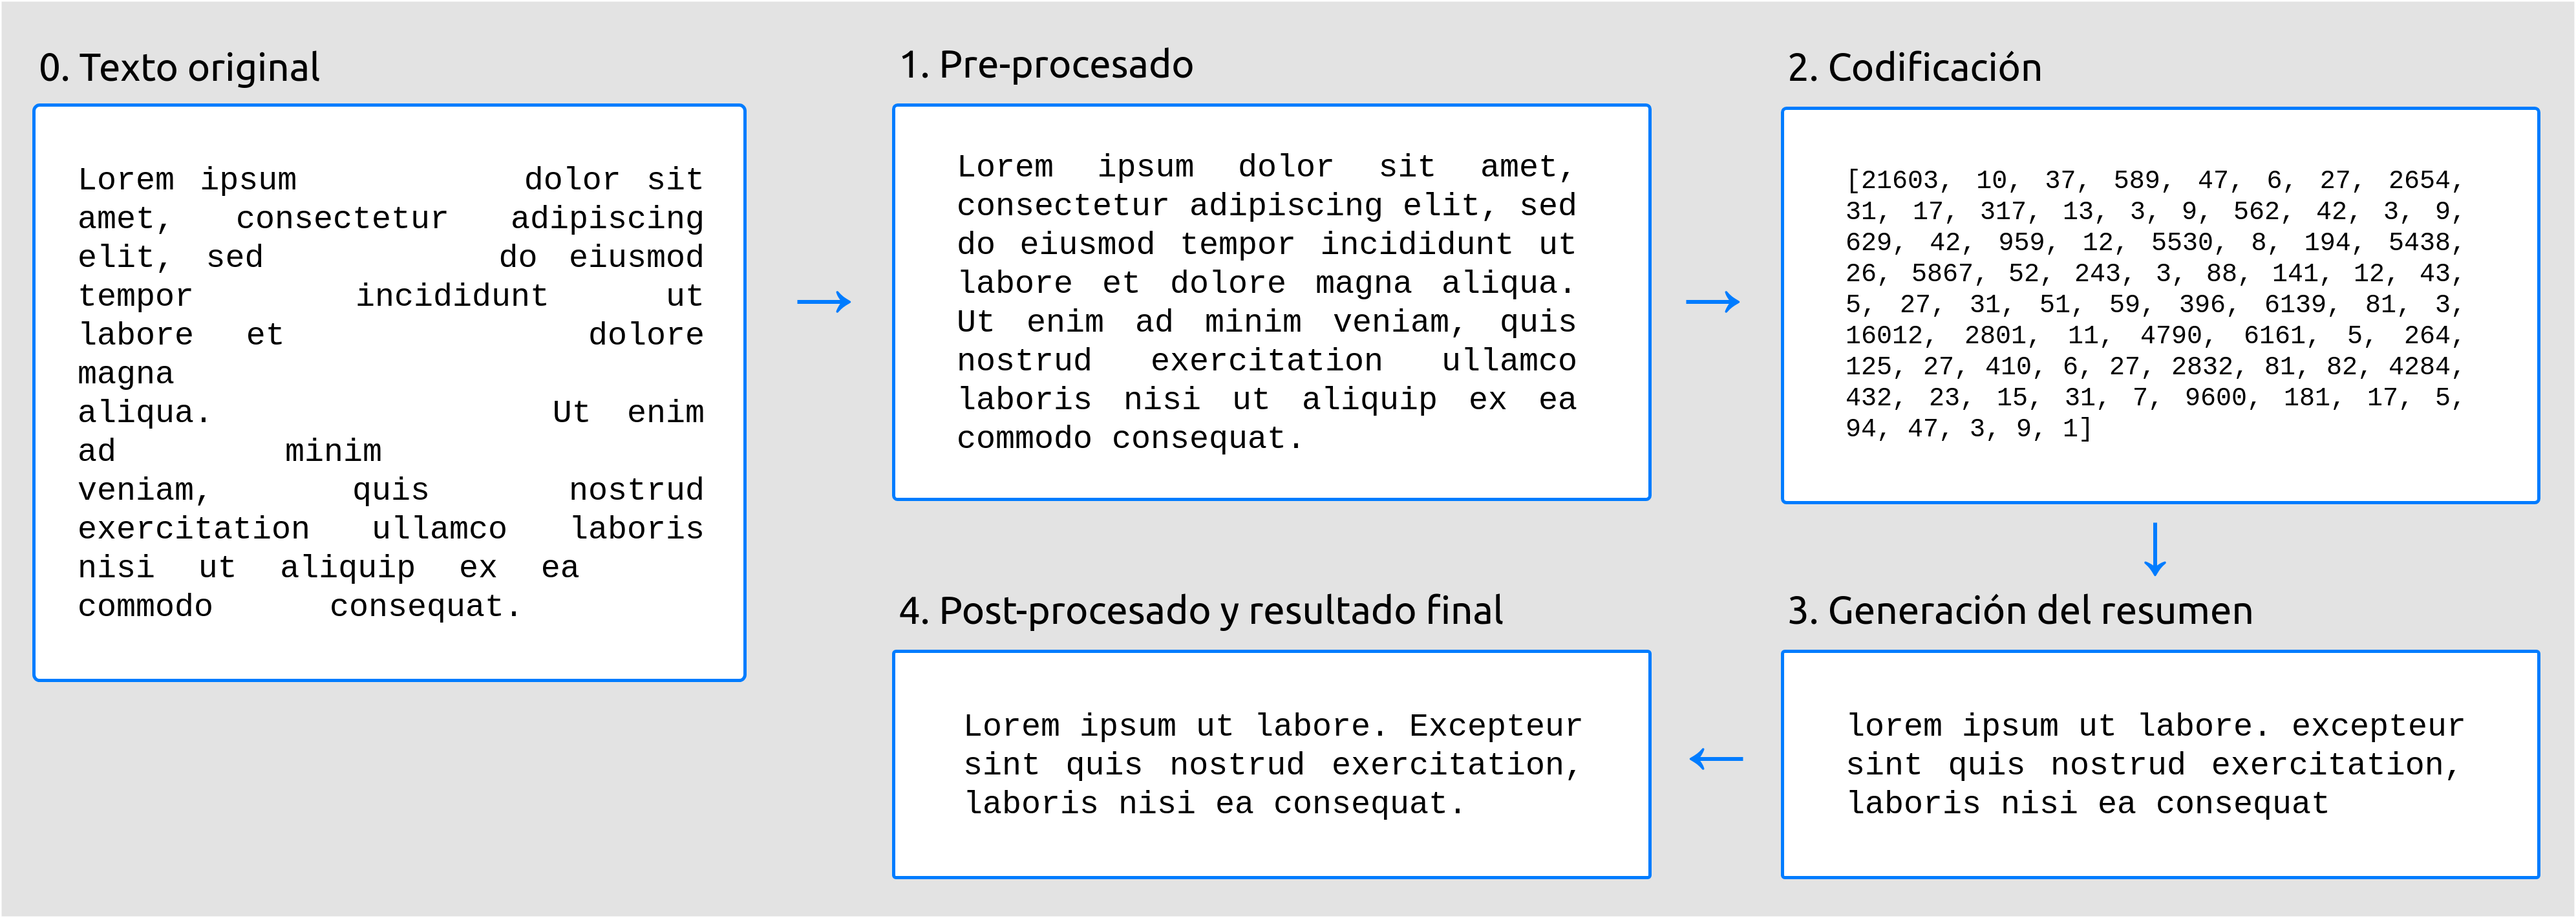
\includegraphics[width=\textwidth]{etapas-resumen}
	\caption{Etapas en la generación de resúmenes.}
	\label{fig:etapas-resumen}
\end{figure}

Veamos en detalle en qué consiste cada una de ellas.

\bigskip
\section{Pre-procesado del texto} \label{sec:preprocesado}

El principal objetivo de esta etapa es adecuar el texto de entrada para que se aproxime lo máximo posible a lo que el modelo espera. Adicionalmente, se separa en texto de entrada en frases. Esta separación puede parecer \emph{a priori} una tarea trivial, pero involucra una serie de dificultades que se detallarán a continuación.

Cabe destacar que, como mencionábamos en la \hyperref[chapter:intro]{Introducción}, los modelos pre-entrenados de los que hacemos uso solo admiten textos en inglés, por lo que algunas de las consideraciones que tomamos en el pre-procesado del texto solo son aplicables a este idioma.

A grandes rasgos, en la etapa de pre-procesado se divide a su vez en los siguientes pasos:

\vspace{-0.4cm}

\begin{itemize}
	\item [\textbullet] Eliminar retornos de carro, tabuladores (\texttt{\textbackslash n}, \texttt{\textbackslash t}) y espacios sobrantes entre palabras (p. ej. \texttt{``I \quad am''} $\rightarrow$ \texttt{``I am''}).
	
	\item [\textbullet] Añadir un espacio al inicio de las frases intermedias (p. ej.: \texttt{``How's it going?Great!''} $\rightarrow$ \texttt{``How's it going? Great!''}. Esto es especialmente relevante en el caso de algunos modelos, como por ejemplo BART \cite{lewis19}, los cuales tienen en cuenta ese espacio inicial para distinguir entre frases iniciales y frases intermedias en la generación de resúmenes\footnote{\, Por el momento, no hacemos uso de este modelo, aunque podría incluirse en el futuro.}.
	
	\item [\textbullet] Establecer un mecanismo que permita llevar a cabo la ya mencionada separación del texto en frases. Esto es importante dado que los modelos tienen un tamaño de entrada máximo. Dos estrategias comunes para eludir esta limitación consisten en (a) truncar el texto de entrada, lo cual puede llevar asociado pérdidas notables de información, o (b) dividir el texto en fragmentos de menor tamaño. En nuestro caso, la primera opción quedó rápidamente descartada ya que los textos que vamos a recibir, por lo general, superarán el tamaño máximo (en caso contrario tendría poco sentido querer generar un resumen). Refiriéndonos, por tanto, a la segunda opción, es frecuente llevar a cabo dicha separación de manera ingenua, únicamente atendiendo al tamaño de entrada máximo. Sin embargo, en nuestro caso decidimos refinar este proceso e implementamos un algoritmo original\footnote{\, Utilizamos el término <<original>> porque no encontramos ningún recurso en el que se tratara este problema, por lo que tuvimos que resolverlo sin apoyos bibliográficos. Esto no quiere decir, sin embargo, que no se hayan implementado estrategias similares en otros problemas diferentes al aquí expuesto.} en el que dicha separación se realiza de tal modo que ninguna frase queda dividida. Para garantizar el éxito de este algoritmo, es fundamental que las frases estén correctamente divididas; el porqué se clarificará en la \hyperref[sec:codificacion]{siguiente sección}, referente a la codificación del texto.
\end{itemize}

A continuación, nos centraremos en el proceso de división del texto en frases. A la hora de llevar a cabo este proceso, debemos tener en cuenta que el texto de entrada podría contener errores ortográficos o gramaticales, por lo que debemos tratar de realizar el mínimo número de suposiciones posibles.

No obstante, la siguiente consideración se nos hace necesaria: el punto (.) indica el final de una frase solo si la siguiente palabra empieza con una letra \emph{y} además mayúscula.

Por ejemplo, en el caso de: \texttt{``Your idea is interesting. However, I would [...].''} se separaría en dos frases, dado que la palabra posterior al punto empieza con una letra mayúscula. Sin embargo: \texttt{``We already mentioned in Section 1.1 that this example shows [...].''} conformaría una única frase, ya que tras el punto no aparece una letra. Procedemos de igual modo en el caso de los signos de interrogación (?) y de exclamación (!). Por ejemplo: \texttt{``She asked \lq How's it going?\rq, and I said \lq Great!\rq.''} se tomará correctamente como una sola frase; tras la interrogación, la siguiente palabra comienza con una letra \emph{minúscula}.
	
Con la suposición anterior, también se agruparían correctamente los puntos suspensivos.

Sin embargo, fallaría en situaciones como: \texttt{``NLP (i.e. Natural Langua}-\texttt{ge Processing) is a subfield of Linguistics, Computer Science, \\ and Artificial Intelligence.''}, en la que la división sería: \texttt{``NLP (i.e.''} por un lado, y \texttt{``Natural Language Processing) is a subfield [...].''}, por otro, ya que \texttt{``Natural''} empieza con mayúscula y aparece tras un punto.

Asimismo, la razón principal por la que no podemos apoyarnos únicamente en reglas predefinidas, reside en las llamadas Entidades Nombradas (\emph{Named Entities}, en inglés), esto es, palabras que hacen referencia a personas, lugares, instituciones, empresas, etc. Existe toda una disciplina dedicada la identificación de este tipo de palabras, conocida como Reconocimiento de Entidades Nombradas (NER, por sus siglas en inglés), y pese a los buenos resultados conseguidos por algunos de los modelos propuestos, se considera un problema lejos de estar resuelto \cite{ner20}.

En nuestro caso emplearemos un modelo pre-entrenado para solucionar, al menos en parte, el problema de las Entidades Nombradas. Este modelo también solventa situaciones como la descrita anteriormente, en las que las reglas escritas a mano se quedan cortas. En el capítulo de \hyperref[chapter:tecnicas]{Técnicas y Herramientas}, hablaremos de dicho modelo y de la implementación concreta en código de los procedimientos expuestos anteriormente.

\bigskip

\section{Codificación del texto} \label{sec:codificacion}

En esta etapa, se lleva a cabo lo que se conoce en inglés como \emph{word embedding}\footnote{\, En el presente documento, hemos traducido este término como <<codificación del texto>>.}. Los modelos de IA trabajan, por lo general, con representaciones númericas. Por ello, las técnicas de \emph{word embedding} se centran en vincular texto (bien sea palabras, frases, etc.), con vectores de números reales \cite{manning19}. Esto hace posible aplicar a la generación de texto arquitecturas comunes dentro de la IA (y especialmente, del \emph{Deep Learning}), como por ejemplo las Redes Neuronales Convolucionales (CNN) \cite{hou20}.

Esta idea, conceptualmente sencilla, encierra una gran complejidad, dado que los vectores generados deben retener la máxima información posible del texto original, incluyendo aspectos semánticos y gramaticales. Por poner un ejemplo, los vectores correspondientes a las palabras <<profesor>> y <<alumno>>, deben preservar cierta relación entre ambos, y a su vez con la palabra <<educación>> o <<escuela>>. Además, su vínculo con las palabras <<enseñar>> o <<aprender>> será ligeramente distinto, dado que en este caso se trata de una categoría gramatical diferente (verbos, en vez de sustantivos). A través de este ejemplo, podemos comprender que se trata de un proceso complejo.

Dado que los modelos pre-entrenados se encargan de realizar esta codificación por nosotros, no entraremos en más detalle en los algoritmos concretos empleados, dado que consideramos que queda fuera del alcance de este trabajo\footnote{\, En cualquier caso, el lector curioso puede explorar los algoritmos más populares de codificación, los cuales, ordenados cronológicamente, son: word2vec \cite{word2vec1, word2vec2}, GloVe \cite{glove14}, y más recientemente, ELMo \cite{elmo18} y BERT \cite{bert18}.}.

Lo que sí hemos tenido que implementar en esta etapa, ha sido la división del texto en fragmentos a fin de no superar el tamaño máximo de entrada del modelo.

De este modo, podremos realizar resúmenes de textos arbitrariamente largos, a través de los siguientes pasos:

\vspace{-\baselineskip}
\begin{enumerate}
	\tightlist
	\item Dividimos el texto en fragmentos.
	\item Generamos un resumen de cada fragmento.
	\item Concatenamos los resúmenes generados.
\end{enumerate}
\vspace{-0.3cm}

Anteriormente, habíamos mencionado el término \emph{token}. Este concepto se puede traducir al español como <<símbolo>>. En nuestro caso concreto, un \emph{token} se corresponde con el vector numérico asociado a una palabra al realizar la codificación. Más concretamente, en modelos más actuales, como el modelo T5 \cite{raffel19}, los \emph{tókenes} pueden referirse a palabras completas o a \emph{fragmentos} de las mismas.

Por lo general, las palabras que aparecen en el vocabulario con el que ha sido entrenado el modelo van a generar un único \emph{token}. Sin embargo, las palabras desconocidas, se descompondrán en varios \emph{tókenes}. Lo mismo sucede con palabras compuestas o formadas a partir de prefijación o sufijación. En la \hyperref[fig:t5-tokenizer]{siguiente figura}, podemos ver un ejemplo de ello:

\begin{figure}[h]
	\centering
	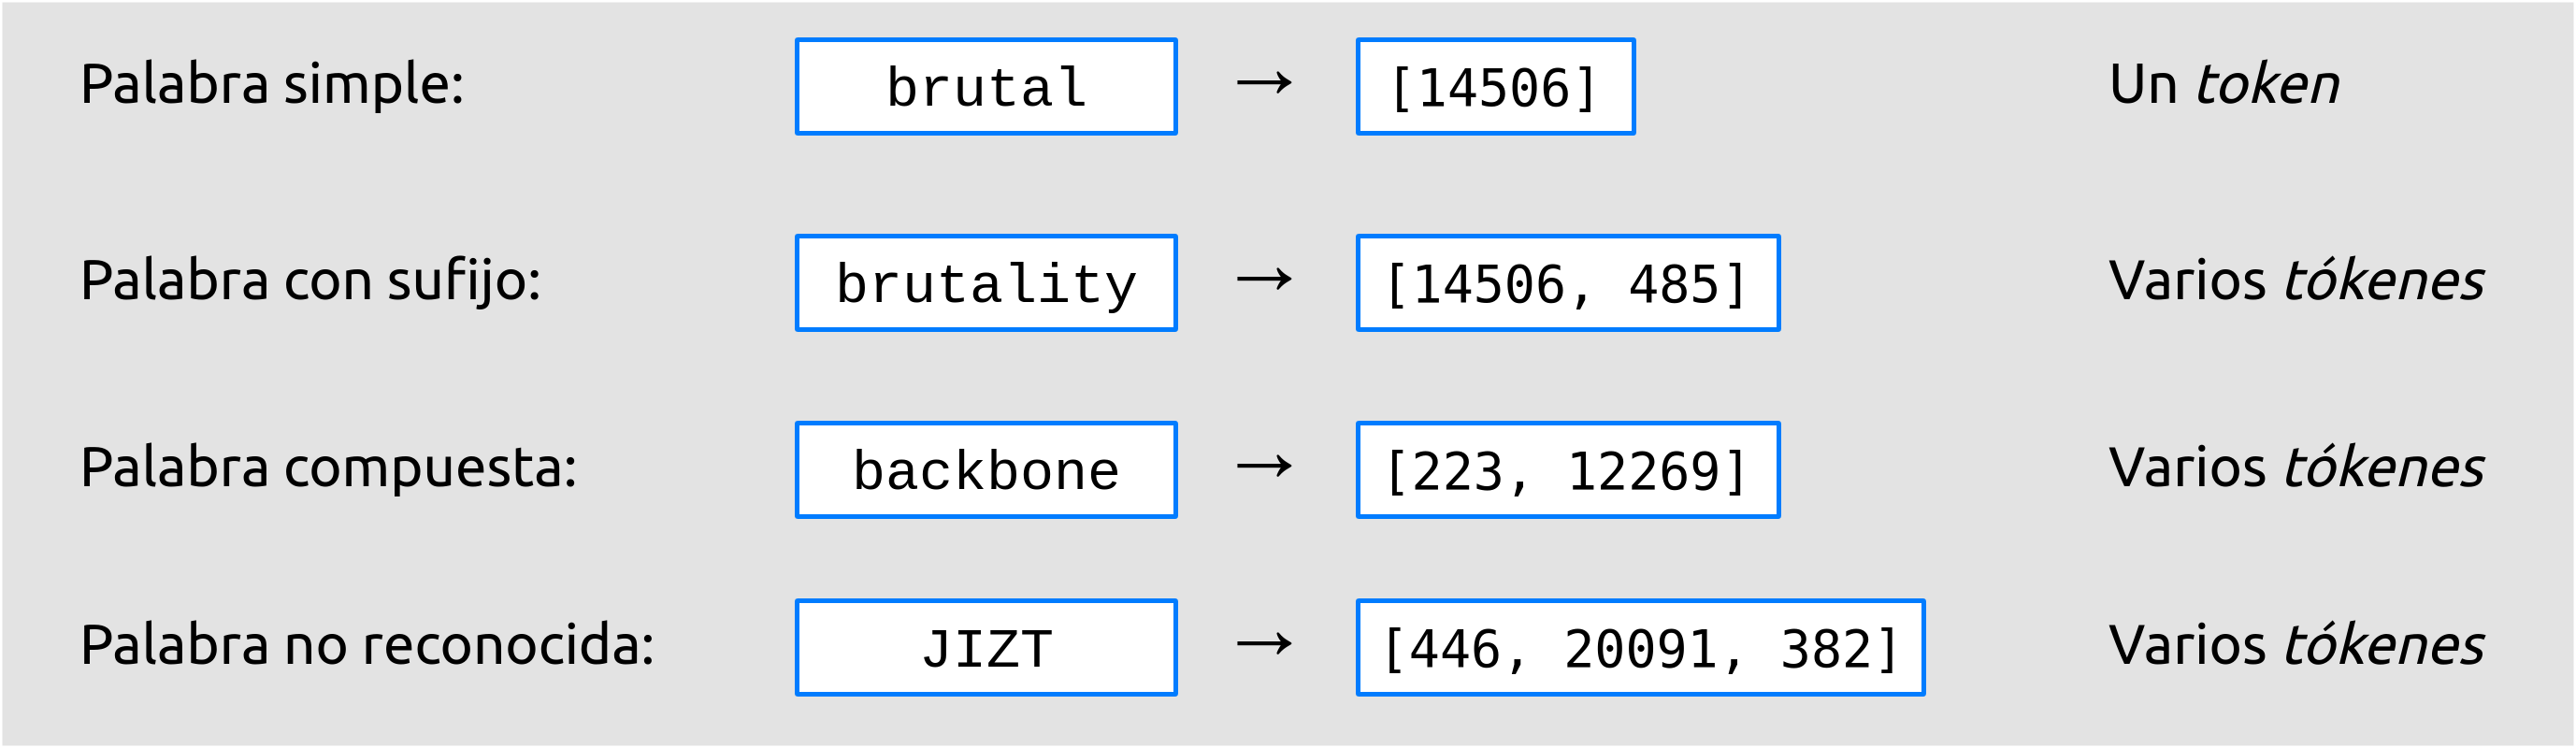
\includegraphics[width=1.035\textwidth]{t5-tokenizer}
	\caption{Ejemplo de \emph{tokenización} con el modelo T5.}
	\label{fig:t5-tokenizer}
\end{figure}

En el anterior ejemplo, si decodificamos los \emph{tókenes} correspondientes a la palabra \texttt{``backcone''}, esto es, \texttt{[223, 12269]}, obtenemos los fragmentos \texttt{``back''}, y \texttt{``bone''}, respectivamente.

La idea detrás de esta fragmentación se basa en la composición, uno de los mecanismos morfológicos de formación de palabras más frecuentes \cite{cetnarowska05} en muchos idiomas, como el inglés, español o alemán. Por tanto, presupone que dividiendo las palabras desconocidas en fragmentos menores, podemos facilitar la comprensión de las mismas. Naturalmente, habrá casos en los que esta idea falle; por ejemplo, en la figura anterior, la palabra \texttt{``JIZT''} se descompone en \texttt{``J''}, \texttt{``IZ''}, \texttt{``T''}, lo cual no parece hacerla mucho más comprensible.

Una vez explicado el concepto de \emph{token}, volvamos al problema ya mencionado con anterioridad: algunos modelos de generación de texto (entre ellos, el T5) admiten un tamaño de entrada máximo, determinado en función del número de \emph{tókens}. Debido a que la unidad de medida es el número de \emph{tókenes}, y no el número de palabras, o de caracteres, debemos tener en cuenta algunos detalles, entre ellos el hecho de que los modelos generan \emph{tókenes} especiales para marcar el inicio y/o el final de la secuencia de entrada.

El modelo T5 (el cual como mencionábamos anteriormente, es el único modelo que utilizamos por ahora), genera un único \emph{token} de finalización de secuencia (EOS, \emph{end-of-sequence}), que se coloca siempre al final del texto de entrada, una vez codificado, y en el caso de de este modelo siempre tiene el \emph{id} 1. En la \hyperref[fig:t5-eos-ejemplo]{siguiente figura} podemos ver un ejemplo con un texto de entrada:

\begin{figure}[h]
	\centering
	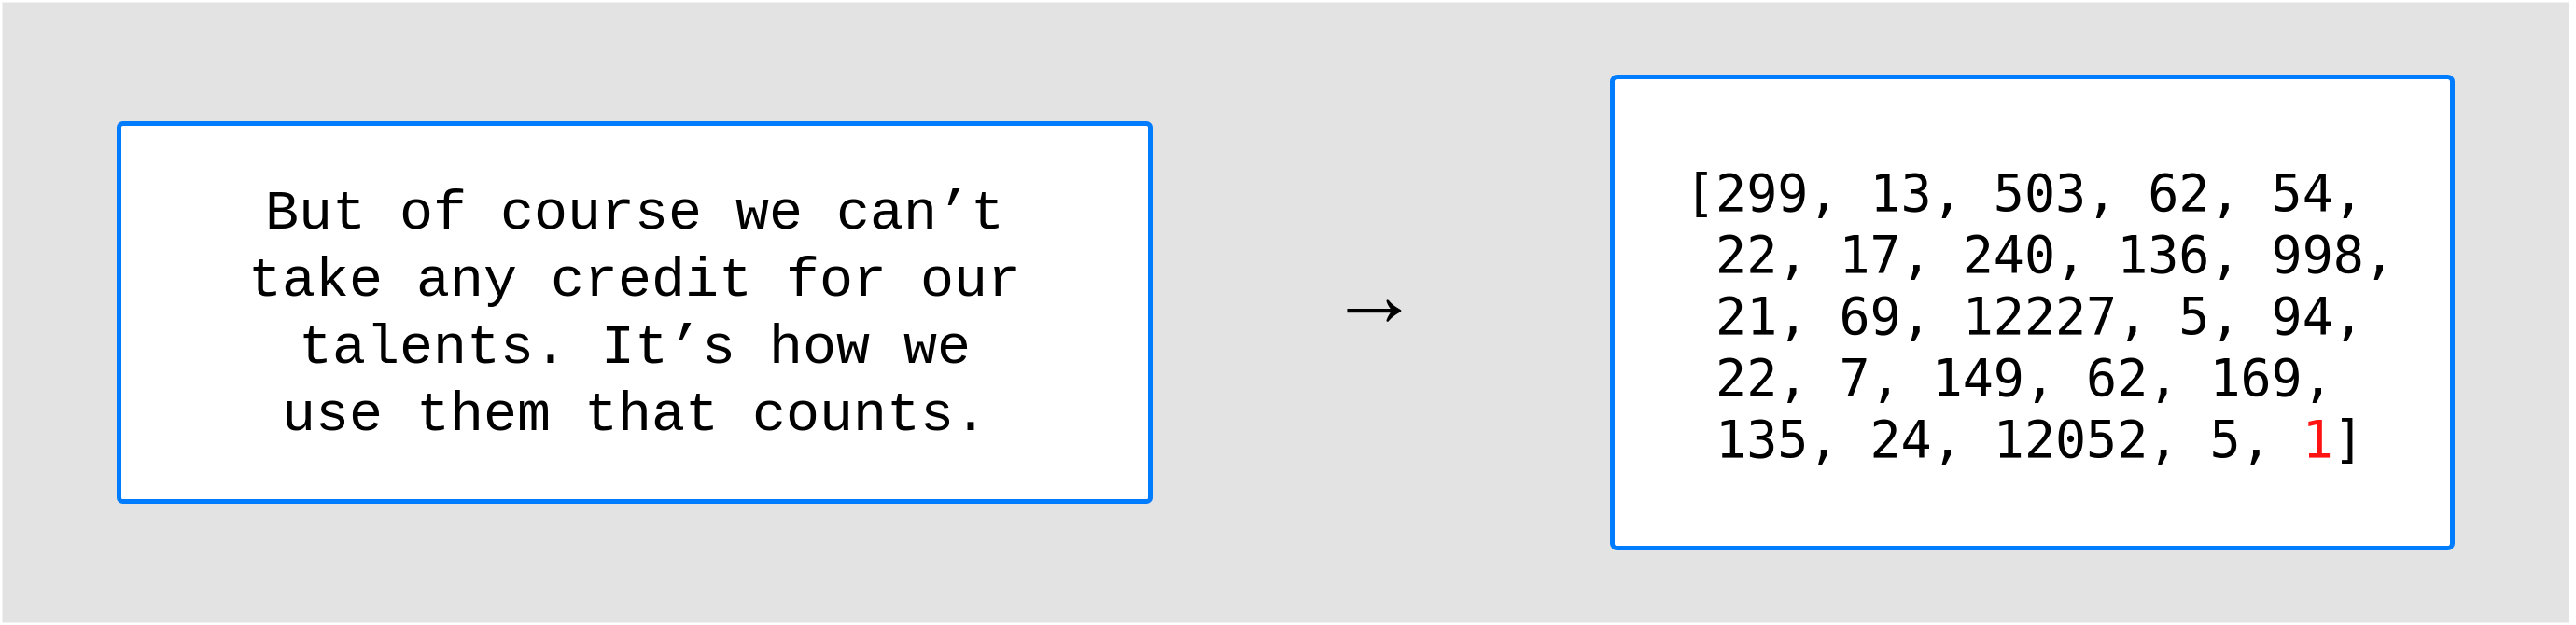
\includegraphics[width=\textwidth]{t5-eos-ejemplo}
	\caption{Pasaje del libro \emph{A Wrinkle in Time}. El \emph{tóken} EOS se ha marcado en rojo.}
	\label{fig:t5-eos-ejemplo}
\end{figure}

Como podemos ver, el \emph{tóken} EOS aparece una única vez por cada texto de entrada, y es independiente de las palabras o frases que este contiene.

Otro aspecto a tener en cuenta, reside en que este modelo no solo es capaz de generar resúmenes, si no que puede ser empleado para otras tareas como la traducción, respuesta de preguntas \cite{raffel19}, etc. Para indicarle cuál de estas es la tarea que queremos que desempeñe, curiosamente se lo tenemos que indicar tal y cómo lo haríamos en la vida real; en nuestro caso, simplemente precedemos el texto a resumir con la orden <<resume>> (<<\emph{summarize}>>). Por poner otro ejemplo, si quisiéramos traducir del alemán al español, le señalaríamos: <<traduce de alemán a español>> seguido de nuestro texto (<<\emph{summarize German to Spanish}>>).

Por consiguiente, este prefijo deberá aparecer al principio de cada una de las subdivisiones generadas y, del mismo modo, deberemos tenerlo en cuenta a la hora de calcular el número de \emph{tókenes} de las mismas.

Con las anteriores consideraciones en mente, el objetivo principal será llevar a cabo la división del texto de entrada de forma que el número de \emph{tókenes} varíe lo mínimo posible entre las diferentes subdivisiones, y todo ello sin partir ninguna frase.

Esta es una tarea más compleja de lo que puede parecer. En nuestro caso, hemos propuesto un \hyperref[alg:division-codificacion]{algoritmo} que emplea una estrategia voraz para llevar a cabo una primera división del texto; posteriormente procede al \emph{balanceo} de las subdivisiones generadas en el paso anterior, de forma que el número de \emph{tókenes} en cada subdivisión sea lo más parecido posible. Y esto, evidentemente, sin superar el máximo tamaño de entrada del modelo en ninguna de las subdivisiones.

\newcommand\CONDITION[2]%
{\begin{tabular}[t]{@{}l@{}}
		#1 #2
 \end{tabular}%
}
\algdef{SE}[WHILE]{While}{EndWhile}[1]%
{\algorithmicwhile\ \CONDITION{#1}{\ \algorithmicdo}}%
{\algorithmicend\ \algorithmicwhile}
\algdef{SE}[FOR]{For}{EndFor}[1]%
{\algorithmicfor\ \CONDITION{#1}{\ \algorithmicdo}}%
{\algorithmicend\ \algorithmicfor}
\algdef{S}[FOR]{ForAll}[1]%
{\algorithmicforall\ \CONDITION{#1}{\ \algorithmicdo}}
\algdef{SE}[REPEAT]{Repeat}{Until}{\algorithmicrepeat}[1]%
{\algorithmicuntil\ \CONDITION{#1}{}}
\algdef{SE}[IF]{If}{EndIf}[1]%
{\algorithmicif\ \CONDITION{#1}{\ \algorithmicthen}}%
{\algorithmicend\ \algorithmicif}%
\algdef{C}[IF]{IF}{ElsIf}[1]%
{\algorithmicelse\ \algorithmicif\ \CONDITION{#1}{\ \algorithmicthen}}
\begin{algorithm}
	\caption{División y codificación del texto.}\label{alg:division-codificacion}
	\begin{algorithmic}[1]
		\Procedure{CodificaciónConDivisión}{$texto, prefijo$}
		\State $frases \gets \text{dividirEnFrases(\textit{texto})}$
		\State $frasesCodif \gets [\,]$ \Comment{Frases codificadas}
		\State $prefijoCodif \gets \text{codifica(\textit{prefijo})}$
		\State $EOSCodif \gets \text{codifica(\textit{EOS})}$ \Comment{Token EOS codificado}
		\State $subdivsCodif \gets [\,]$ \Comment{Subdivisiones codificadas}
		
		\For{$\textit{fr} \enspace\text{\textbf{in}}\; \textit{frases}$}
			\State $frasesCodif \gets \text{codifica(\textit{fr})}[:-1]$ \Comment{Excluir EOS}
		\EndFor
		
		\State $ptosCorte \gets \text{divideVoraz(\textit{frasesCodif}, \textit{prefijoCodif})}$
		
		\State $ptosCorte \gets \text{balanceaSubdivs(\textit{ptosCorte})}$

		\For{$i \gets 0, \text{len(\textit{ptosCorte}) - 1}$}
			\State $frasesSubvid \gets frasesCodif[ptosCorte[i]:ptosCorte[i+1]]$ \Comment{Frases en subdiv.}
			\State $subdivsCodif[i] \gets \text{concatena(\textit{prefijoCodif}, \textit{frasesSubdiv}, \textit{EOSCodif})}$
		\EndFor
		\State \textbf{return} $subdivsCodif$
		\State \hspace{-0.5cm}\textbf{end procedure}
		\EndProcedure
	\end{algorithmic}
\end{algorithm}

Este algoritmo devuelve las subdivisiones en las que se ha separado el texto, ya codificadas. Por tanto, $subdivsCofif$ tendrá la siguiente forma:

\vspace{-0.5cm}

\[ [[23, 34, 543, 45, ..., 1], [23, 32. 401, 11, ..., 1], [23, 74. 25, 204, ..., 1], ...] \]

Es decir, cada una de las listas contenidas en $subdivsCodif$ contiene los \emph{tókenes} correspondientes a dicha subdivisión, con el prefijo (23) y el \emph{token} EOS (1) añadidos.
	
La lógica detrás de la función $divideVoraz$ es la siguiente:

\begin{algorithm}
	\caption{División voraz del texto.}\label{alg:divide-voraz}
	\begin{algorithmic}[1]
		\Procedure{DivideVoraz}{$frasesCodif, prefijoCodif$}
		\State $ptosCorte \gets [0]$
		\State $lenSubdiv = \text{len(\textit{prefijoCodif})} + \text{len(\textit{frasesCodif}[0])} + 1$ \Comment Contar prefijo y EOS
		\For{$i \gets 0, \text{len(\textit{frasesCodif}) - 1}$}
			\State $lenSubdiv = lenSubdiv + \text{len(\textit{frasesCodif}[i])}$
			\If{lenSubdiv > \, model.maxLength}
				\State $ptosCorte.\text{añadir(\textit{i})}$
				\State $lenSubdiv = \text{len(\textit{prefijoCodif})} + \text{len(\textit{frasesCodif}[i])} + 1$
			\EndIf
		\EndFor
		\State $ptosCorte.\text{añadir(len(\textit{frasesCodif}))}$
		\State \textbf{return} $ptosCorte$
		\State \hspace{-0.5cm}\textbf{end procedure}
		\EndProcedure
	\end{algorithmic}
\end{algorithm}

Es decir, $ptosCorte$ será una lista que indique los índices que delimitan cada subdivisión, por ejemplo:

\vspace{-0.5cm}

\[ [0, 45, 91, 130, 179, 190] \]

En este caso, la primera subdivisión iría desde la frase 0 hasta la 45, la segunda subdivisión de la 46 a la 91, la tercera de la 92 a la 130, y así sucesivamente.

Como podemos ver en el ejemplo, el número de \emph{tókenes} por subdivisión está en torno a los 45, menos en la última subdivisión que solo contiene 10 \emph{tókenes} ($190-180$). Debido a la propia naturaleza del algoritmo voraz, será siempre la última subdivisión la que pueda contener un número de \emph{tókenes} muy por debajo de la media, lo que puede causar que el resumen de está última subdivisión sea demasiado corto (o incluso sea la cadena vacía). Para evitar esto, balanceamos las subdivisiones, de forma que el número de \emph{tókenes} en cada una de ellas esté equilibrado.


\algdef{SE}[DOWHILE]{Do}{DoWhile}{\algorithmicdo}[1]{\algorithmicwhile\ #1}%
\begin{algorithm}
	\caption{Balanceo de las subdivisiones.}\label{alg:balancea-subdivs}
	\begin{algorithmic}[1]
		\Procedure{BalanceaSubdivs}{$ptosCorte$}
		\State $ptosCorteBalan \gets ptosCorte$ \Comment{Puntos de corte balanceados}

		\Do
			\State $ptosCorteBalanOld \gets ptosCorteBalan$
			\For{$i \gets \text{len(\textit{ptosCorteBalan})} - 1, 1, step: - 1$} \Comment{Empezar por última subdiv.}
			\State $\textit{diffLen} \gets \text{lenSubdiv(\textit{i} -1)} - \text{lenSubdiv(\textit{i})}$ \Comment{Diferencia en n. de \emph{tókenes}}
			\While{$\textit{diffLen} > 0$}
				\State $últimaFrase \gets \text{getÚltimaFrase(getSubdiv(\textit{i}-1))}$
				
				\If{$\text{getSubdiv(\textit{i}) + len(\textit{últimaFrase}) <= model.maxLength} \enspace \wedge$ \\ \hspace{0.5cm} $\text{len(\textit{últimaFrase}) <= \textit{diffLen}}$}
				\State $\text{mueveÚltimaFrase(getSubdiv(\textit{i}-1), getSubdiv(\textit{i}))}$
				\State $ptosCorteBalan[i-1] \gets ptosCorteBalan[i-1] - 1$
				\Else \\ \hspace{2.42cm}\textbf{\emph{break}}
				\EndIf
			\EndWhile
			\EndFor
		\DoWhile{$ptosCorteBalan \not = ptosCorteBalanOld$}
		\State \textbf{return} $ptosCorte$
		\State \hspace{-0.5cm}\textbf{end procedure}
		\EndProcedure
	\end{algorithmic}
\end{algorithm}

En esencia, lo que este último algoritmo hace es comparar la diferencia en número de \emph{tókenes} entre subdivisiones consecutivas, empezando por el final, de forma que primero se compara la penúltima con la última subdivisión, después la antepenúltima con la penúltima, y así sucesivamente. Si es necesario, va moviendo frases completas desde una subdivisión a la siguiente, por ejemplo, desde la penúltima a la última subdivisión. Este algoritmo tiene una complejidad en el peor de los casos de $O(n^3)$, siendo $n$ el número de subdivisiones.

Podemos visualizarlo gráficamente con un ejemplo muy simple:

\begin{figure}[h]
	\centering
	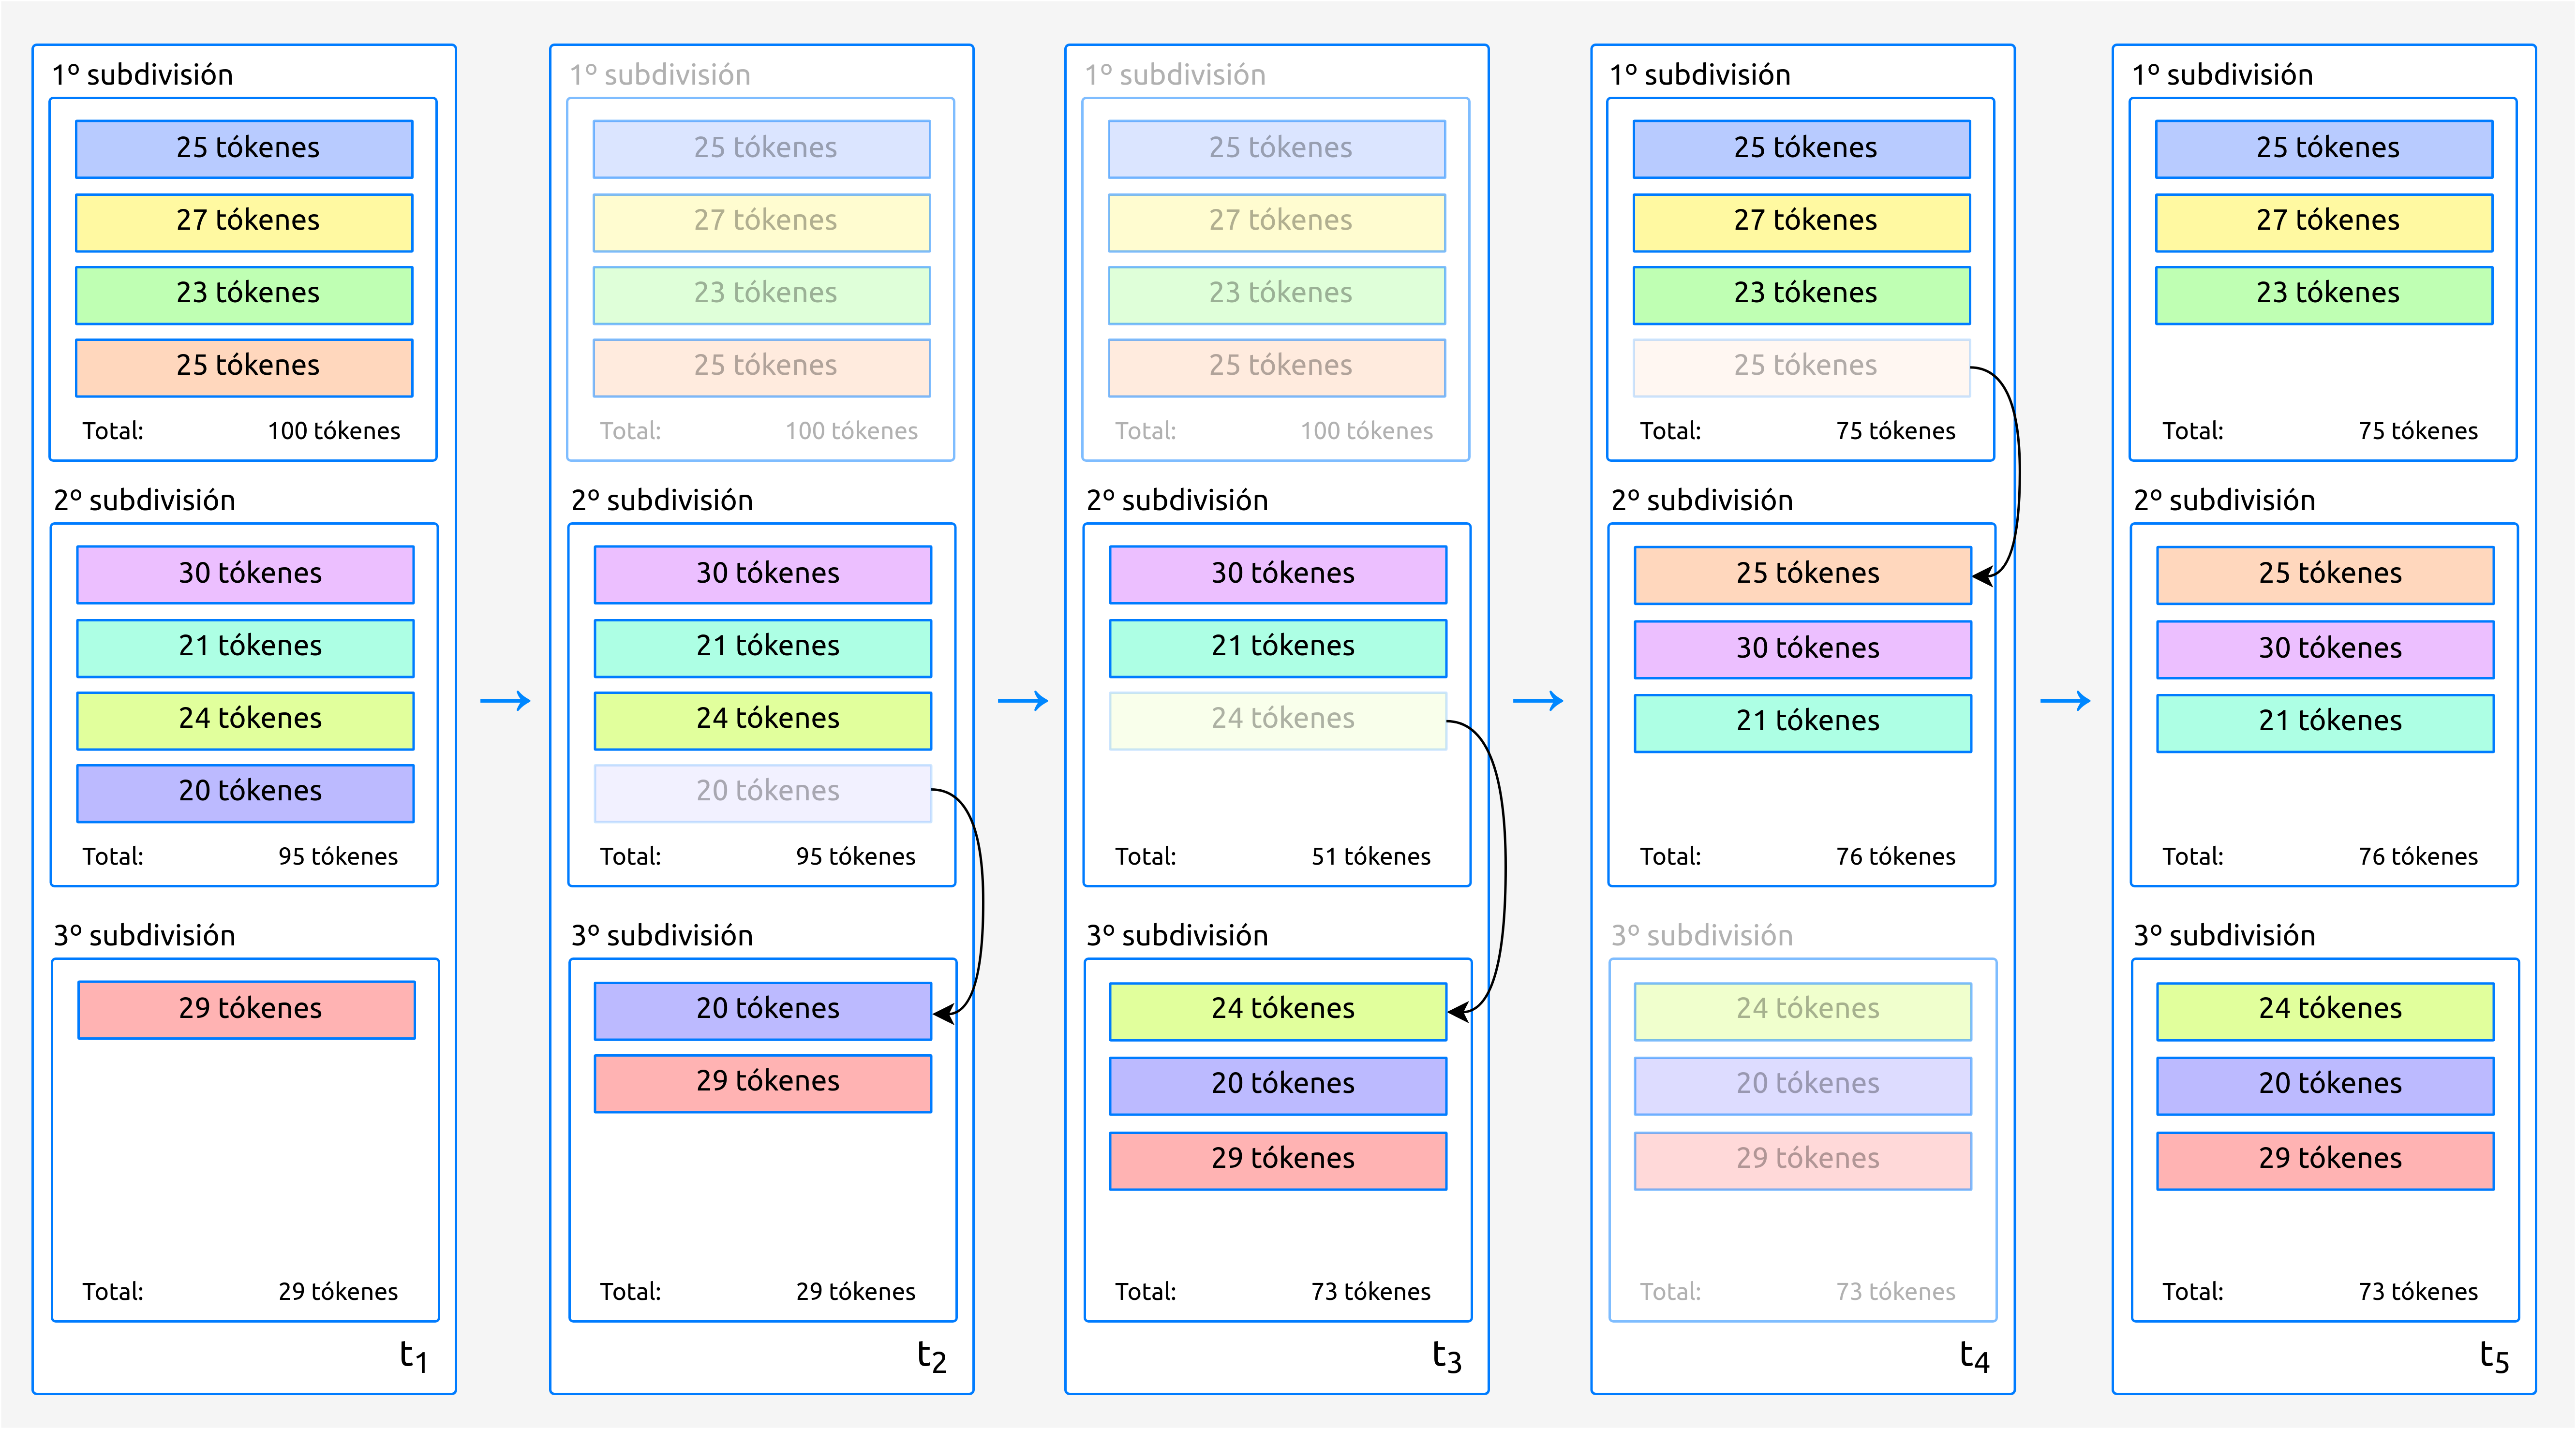
\includegraphics[width=\textwidth]{algoritmo-balanceo}
	\caption{Ejemplo gráfico del algoritmo de balanceo. Las desviación estándar del número de \emph{tókenes} de cada frase en $t_1$ es $\sigma_1 = 39.63$ y en $t_5$, acaba siendo $\sigma_5 = 1.53$.}
	\label{fig:algoritmo-balanceo}
\end{figure}

\newpage

\section{Generación del resumen} \label{sec:resumen}

Una vez codificado y dividido el texto apropiadamente, generamos los resúmenes parciales para posteriormente unirlos, dando lugar a un único resumen del texto completo.

En la \autoref{fig:proceso-resumen}, podemos ver los pasos llevados a cabo tanto en la anterior etapa, la codificación y división del texto, como en esta, la generación del resumen.

\begin{figure}[h]
	\centering
	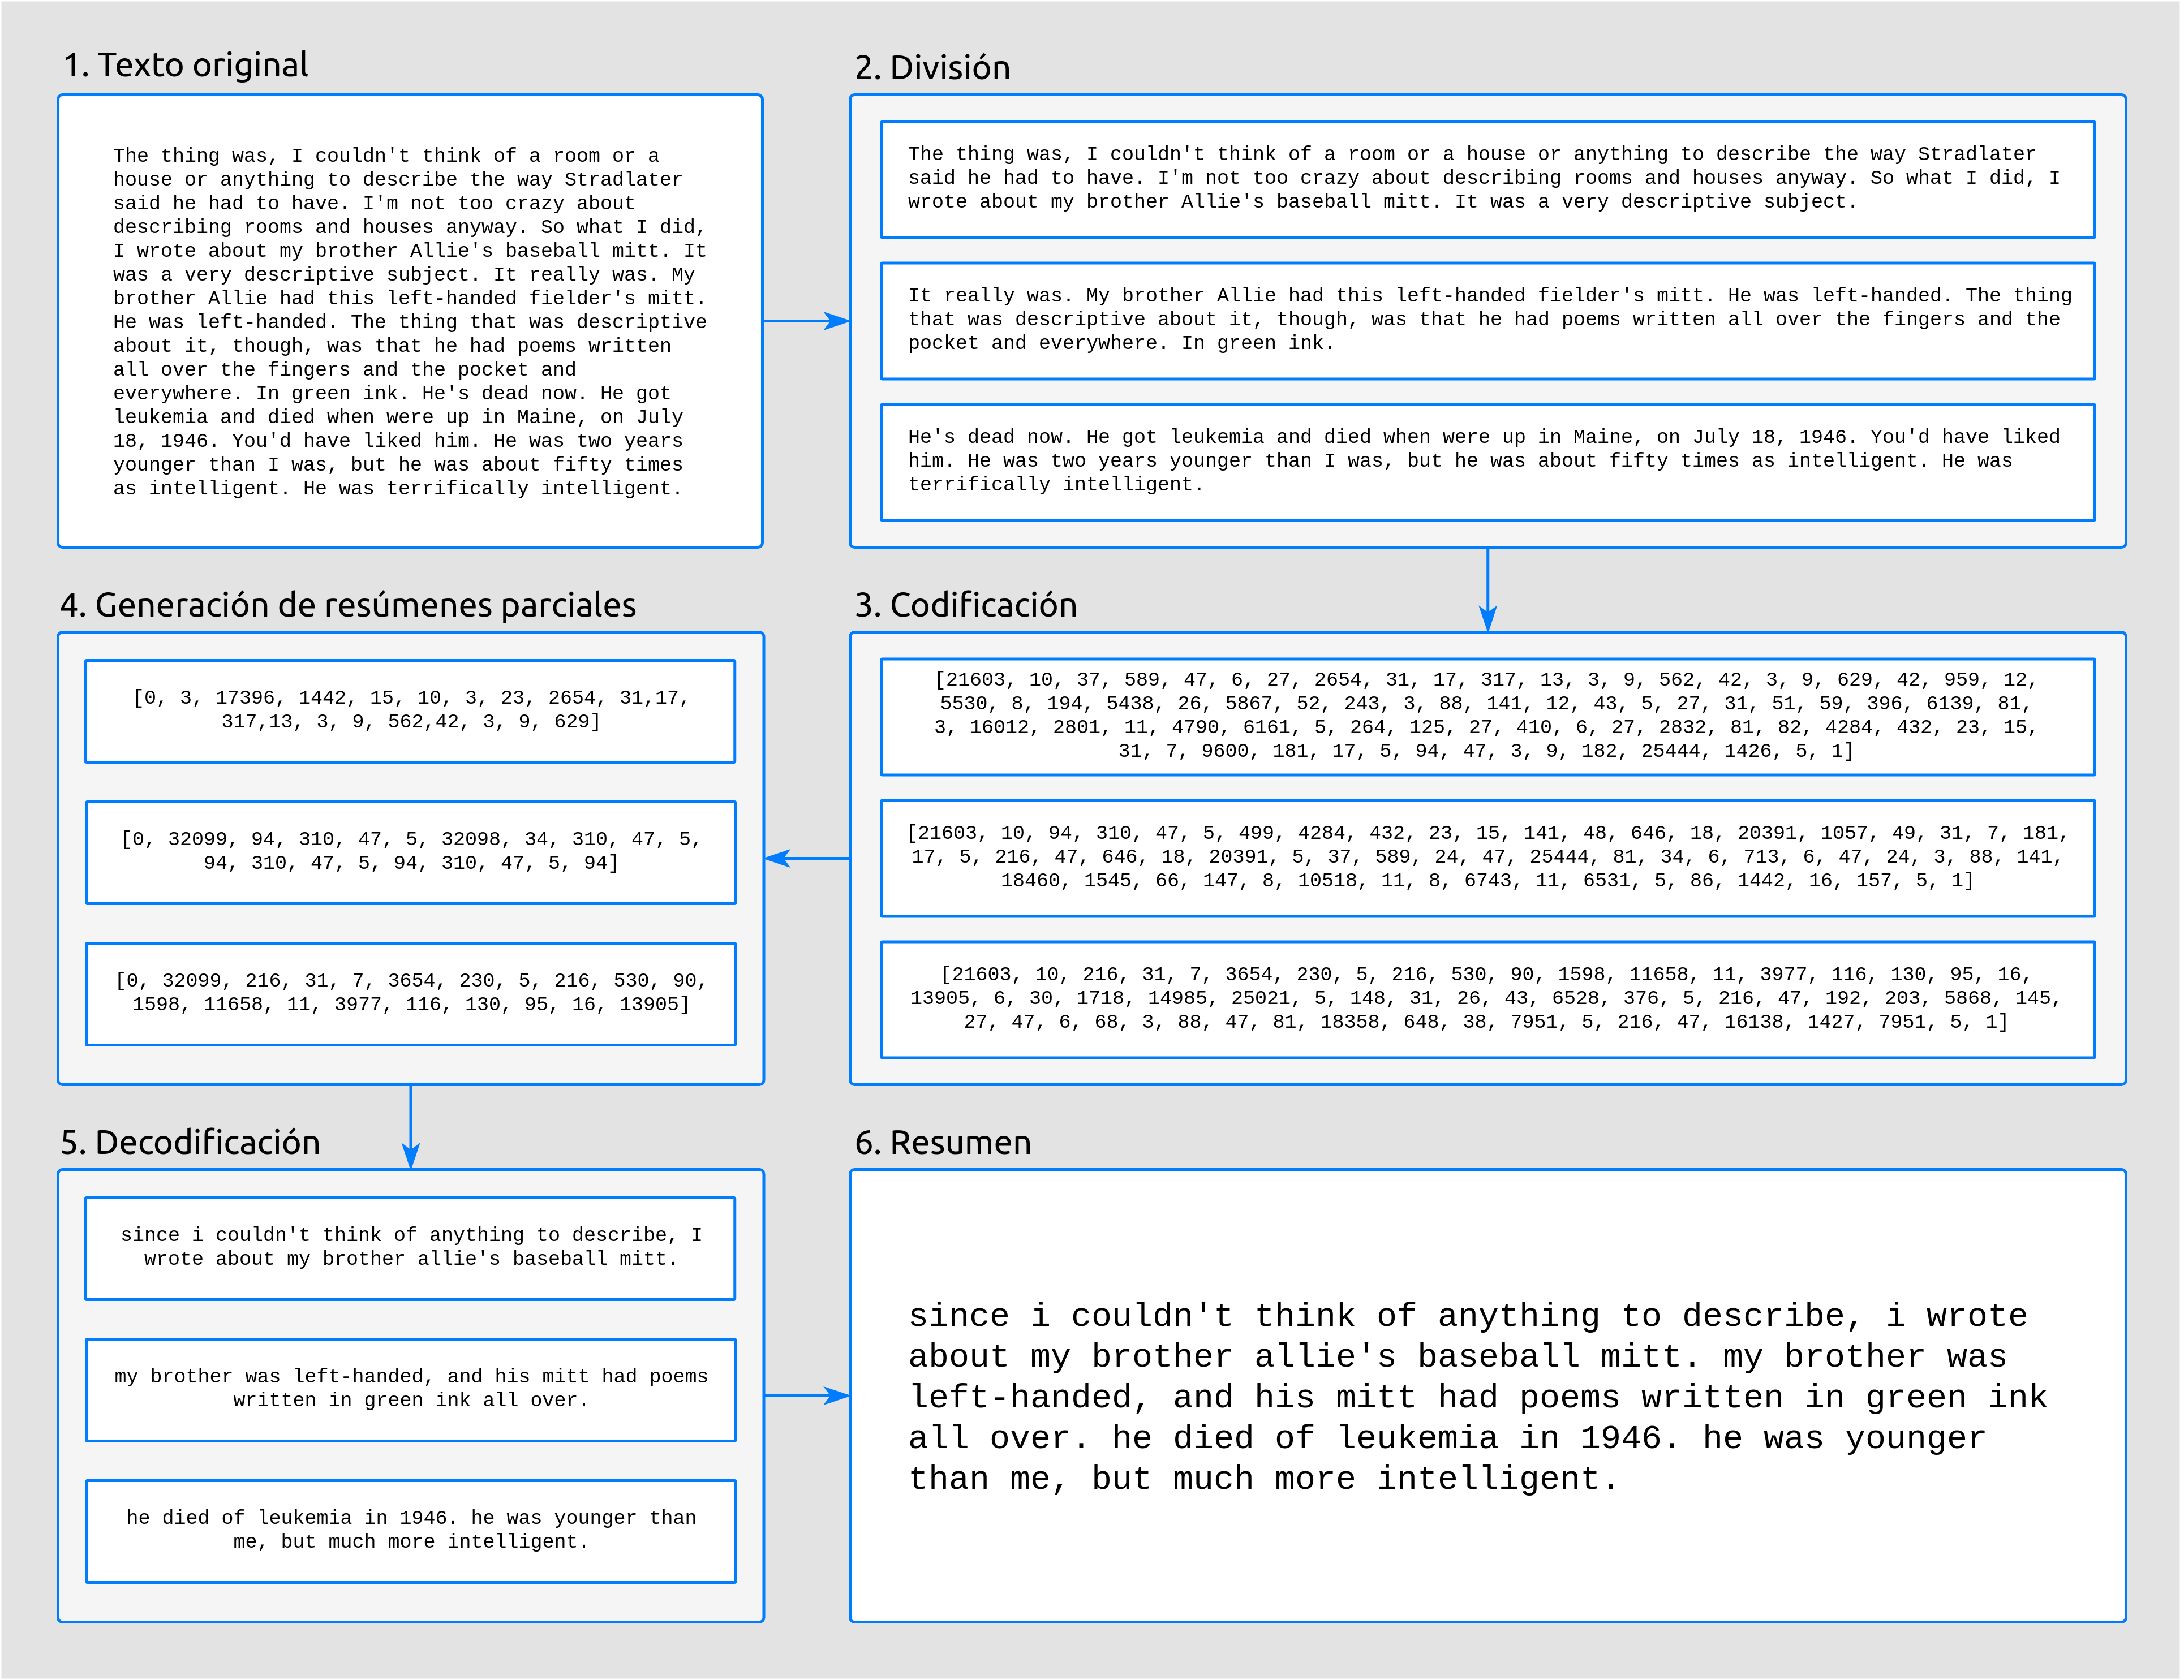
\includegraphics[width=\textwidth]{t5-proceso-resumen}
	\caption{Proceso de generación de resúmenes, ilustrado con un fragmento del libro \emph{The Catcher in the Rye}.}
	\label{fig:proceso-resumen}	
\end{figure}

Como podemos apreciar en la anterior figura, el modelo generador de resúmenes toma el texto codificado, y devuelve una versión reducida del mismo, también codificado. Por ello, antes de poder unir y devolver el resumen generado, debemos realizar un paso de \emph{decodificación}, que realiza el proceso contrario a la \emph{codificación}, como veíamos en la \hyperref[sec:codificacion]{anterior sección}. Algo con lo que tendremos que lidiar en la siguiente etapa, el post-procesado, será corregir el resumen generado para que se ajuste a las reglas ortográficas vigentes, en especial en lo relativo al uso de mayúsculas.

La ventaja de utilizar modelos pre-entrenados es clara: estos modelos son para nosotros cajas negras, a las que solo tenemos que encargarnos de proporcionarles la entrada en el formato concreto que esperan.

Cabe destacar que, el hecho de realizar la división del texto de esta manera, sin atender a aspectos semánticos, podría resultar en que en frases estrechamente relacionadas acabaran en distintas subdivisiones. Por ejemplo, en la \autoref{fig:proceso-resumen}, la frase final de uno de las subdivisiones es: \emph{<<It was a very descriptive subject>>} (<<Era un tema muy descriptivo>>), a la cual le sigue, ya en la siguiente subdivisión: \emph{<<It really was>>} (<<De veras que lo era>>), aludiendo a la anterior frase.

Estos casos son difíciles de resolver. Una posible idea sería tratar de determinar si una frase está relacionada con la anterior, quizás mediante el uso de otro modelo, y de ser así, tratar de mantenerlas en una misma subdivisión, a fin de que el resumen final mantenga la máxima cohesión y coherencia posibles. Esto incrementaría, no obstante, los tiempos de generación de resúmenes. Por ahora, creemos que los resultados obtenidos son lo suficientemente buenos.

\bigskip
\subsubsection{Modelo empleado para la generación de resúmenes: T5}

Come hemos mencionado previamente, JIZT hace uso del modelo T5 \cite{raffel19} de Google. Este modelo fue introducido en el artículo \emph{Exploring the Limits of Transfer Learning with a Unified Text-to-Text Transformer}, presentado en 2019. En él, Colin Raffel \emph{et al.} estudian las ventajas de la técnica del aprendizaje por transferencia (\emph{transfer learning}) al campo del Procesamiento del Lenguaje Natural (NLP).

Tradicionalmente, cada nuevo modelo se entrenaba desde cero. Esto ha cambiado con la inclusión del aprendizaje por transferencia; actualmente, la tendencia es emplear modelos pre-entrenados como punto de partida para la construcción de nuevos modelos.

Las tres principales ventajas del empleo del aprendizaje por transferencia son \cite{sarkar18}:

\vspace*{-\baselineskip}
\begin{itemize}
	\item [\textbullet] Mejora del rendimiento de partida. El hecho de comenzar con un modelo pre-entrenado en vez de un modelo ignorante (\emph{ignorant learner}), proporciona un rendimiento base desde el primer momento.
	
	\item [\textbullet] Disminución del tiempo de desarrollo del modelo, consecuencia del punto anterior.
	
	\item [\textbullet] Mejora del rendimiento final. Esta mejora ha sido estudiada tanto en el caso del NLP \cite{kumar21}, como de otros ámbitos, como la visión artificial \cite{ali21}, o el campo de la medicina \cite{liu21}.
\end{itemize}

La principal novedad de este artículo se encuentra en su propuesta de tratar todos los problemas de procesamiento de texto como problemas texto a texto (\emph{text-to-text}), es decir, tomar un texto como entrada, y producir un nuevo texto como salida. Esto permite crear un modelo general, al que han bautizado como T5, capaz de llevar a cabo diversas tareas de NLP, como muestra el siguiente diagrama:

\bigskip

\imagen{t5-paper}{El \emph{framework} texto a texto permite emplear el mismo modelo, con los mismos hiperparámetros, función de pérdida, etc., para aplicarlo a diversas tareas de NLP \cite{raffel19}.}

En cualquier caso, se puede realizar un ajuste fino del modelo para una de las tareas, a fin de mejorar su rendimiento en dicha tarea específica.

Las posibilidades que este modelo nos ofrece son muy interesantes, dado que en un futuro, nuestro proyecto podría incluir otras tareas de Procesamiento de Lenguaje Natural, haciendo uso de un solo modelo.


\bigskip
\subsubsection{Principales estrategias de generación de resúmenes} \label{subsec:estrategias-gen}

JIZT permite al usuario avanzado configurar de manera precisa los parámetros con los que se genera el resumen. En este apartado, exploraremos las diferentes técnicas con las que se pueden generar resúmenes.

La generación de lenguaje, en general, se basa en la auto-regresión, la cual parte del supuesto de que la distribución de probabilidad de una secuencia de palabras puede descomponerse en el producto de las distribuciones de probabilidades  condicionales de las palabras sucesivas \cite{platen20}. Expresado matemáticamente:

\[ P(w_{1:t} | W_0) = \prod_{t=1}^{T} P(w_t | w_{1:t-1}, W_0), \; siendo \enspace w_{1:0} = \emptyset \]

donde $W_0$ es la secuencia inicial de \emph{contexto}. En nuestro caso, esa secuencia inicial va a ser el propio texto de entrada. La longitud de $T$ no se puede conocer de antemano, dado que se corresponde con el momento $t = T$ en el que el modelo genera el \emph{token} de finalización de secuencia ()EOS), mencionado anteriormente.

Una vez introducido el concepto de auto-regresión, podemos explicar brevemente las cinco	 principales estrategias de generación de lenguaje, las cuales se pueden aplicar todas ellas a la generación de resúmenes: búsqueda voraz, \emph{beam search}, muestreo, muestreo \emph{top-k}, y muestreo \emph{top-p}.

\bigskip
\noindent
\textbf{Búsqueda voraz}

La búsqueda voraz, en cada paso, simplemente selecciona la palabra con mayor probabilidad de ser la siguiente, es decir, $ w_t = argmax_w P(w|w_{t-1}) $ para cada paso \emph{t}.

\begin{figure}[h]
	\centering
	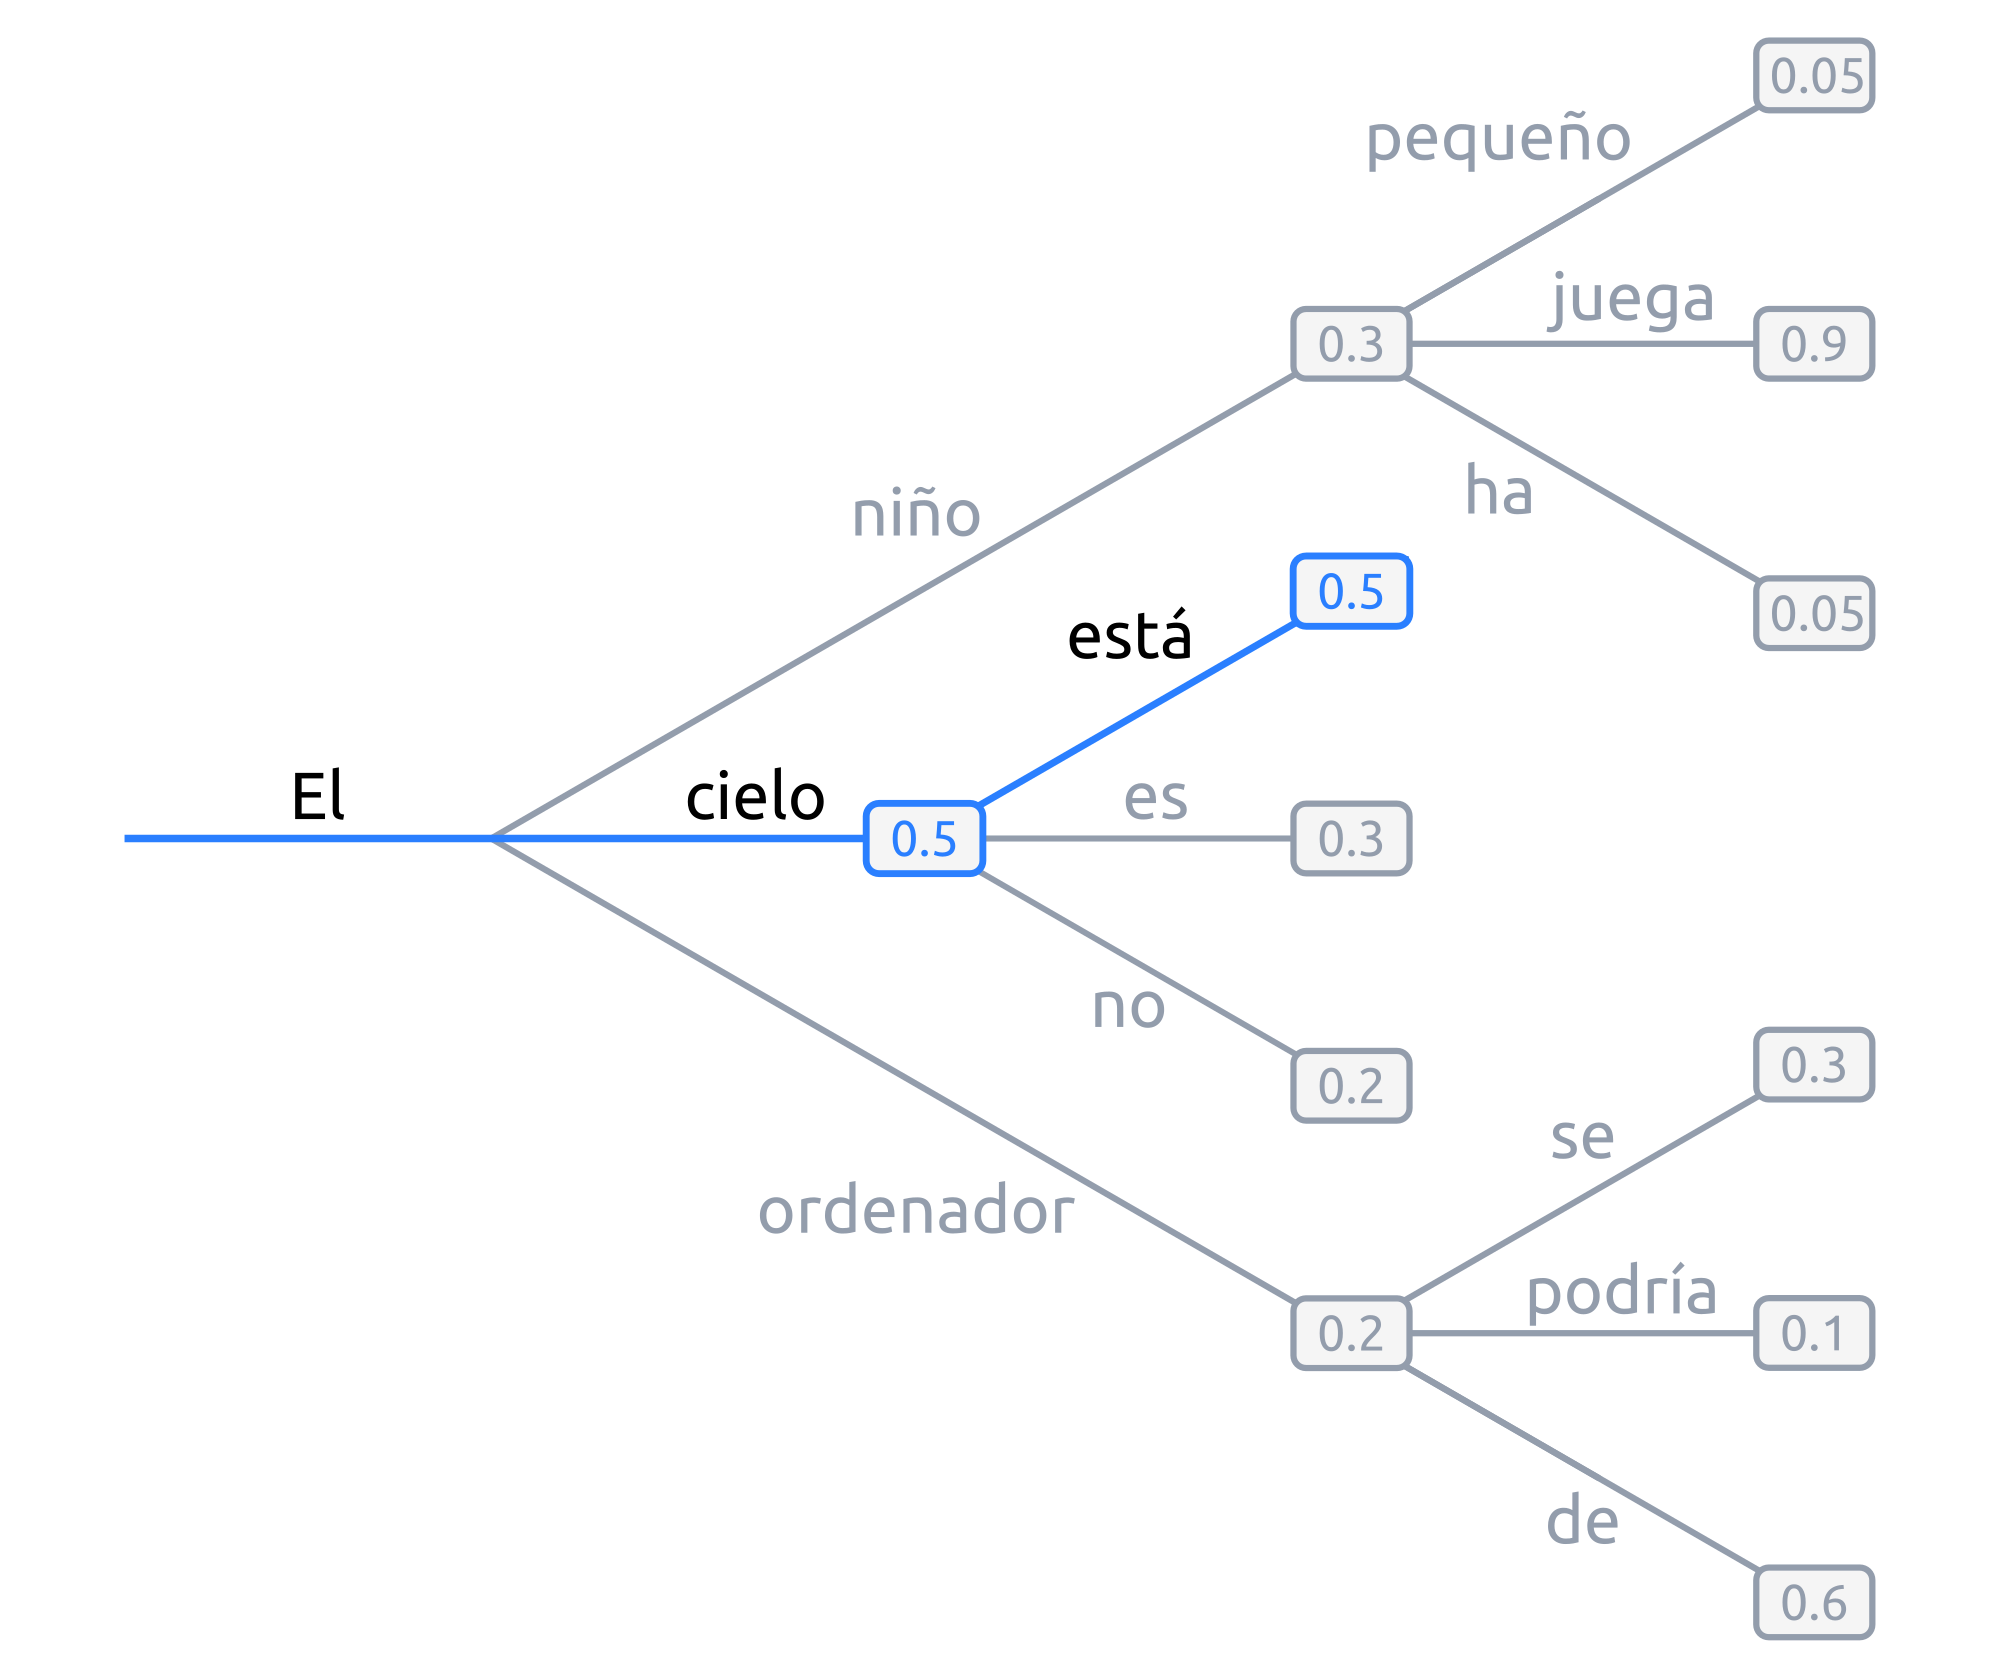
\includegraphics[width=0.7\textwidth]{greedy-search}
	\caption{Ejemplo de búsqueda voraz: en cada paso, se toma la palabra con mayor probabilidad.}
\end{figure}


Por ejemplo, dada la palabra \texttt{``El''}, la siguiente palabra elegida sería \texttt{``cielo''}, por ser la palabra con mayor probabilidad (0.5), y a continuación \texttt{``está''} (0.5), y así sucesivamente.

Este tipo de generación tiene dos problemas principales:

\begin{itemize}
	\item [\textbullet] Los modelos, llegados a cierto punto, comienzan a repetir las mismas palabras una y otra vez. En realidad, esto es un problema que afecta a todos los modelos de generación, pero especialmente a los que emplean búsqueda voraz y \emph{beam search} \cite{vijayakumar16, shao17}.
	\item [\textbullet] Palabras con probabilidades altas pueden quedar enmascaradas tras otras con probabilidades bajas. Por ejemplo, en el anterior anterior ejemplo, la secuencia \texttt{``El niño juega''} nunca se dará, porque a pesar de que \texttt{``juega''} presenta una probabilidad muy alta (0.9), está precedida por \texttt{`niño''}, la cual no será escogida por tener una probabilidad baja (0.3).
\end{itemize}


\bigskip
\noindent
\textbf{\emph{Beam search}}

En este caso, durante el proceso de generación se consideran varios caminos simultáneamente, y finalmente se escoge aquel camino que presenta una mayor probabilidad conjunta. En la \hyperref[fig:beam-search]{siguiente figura} se ilustra un ejemplo con dos caminos (\texttt{num\_beams = 2}).

\begin{figure}[!h]
	\centering
	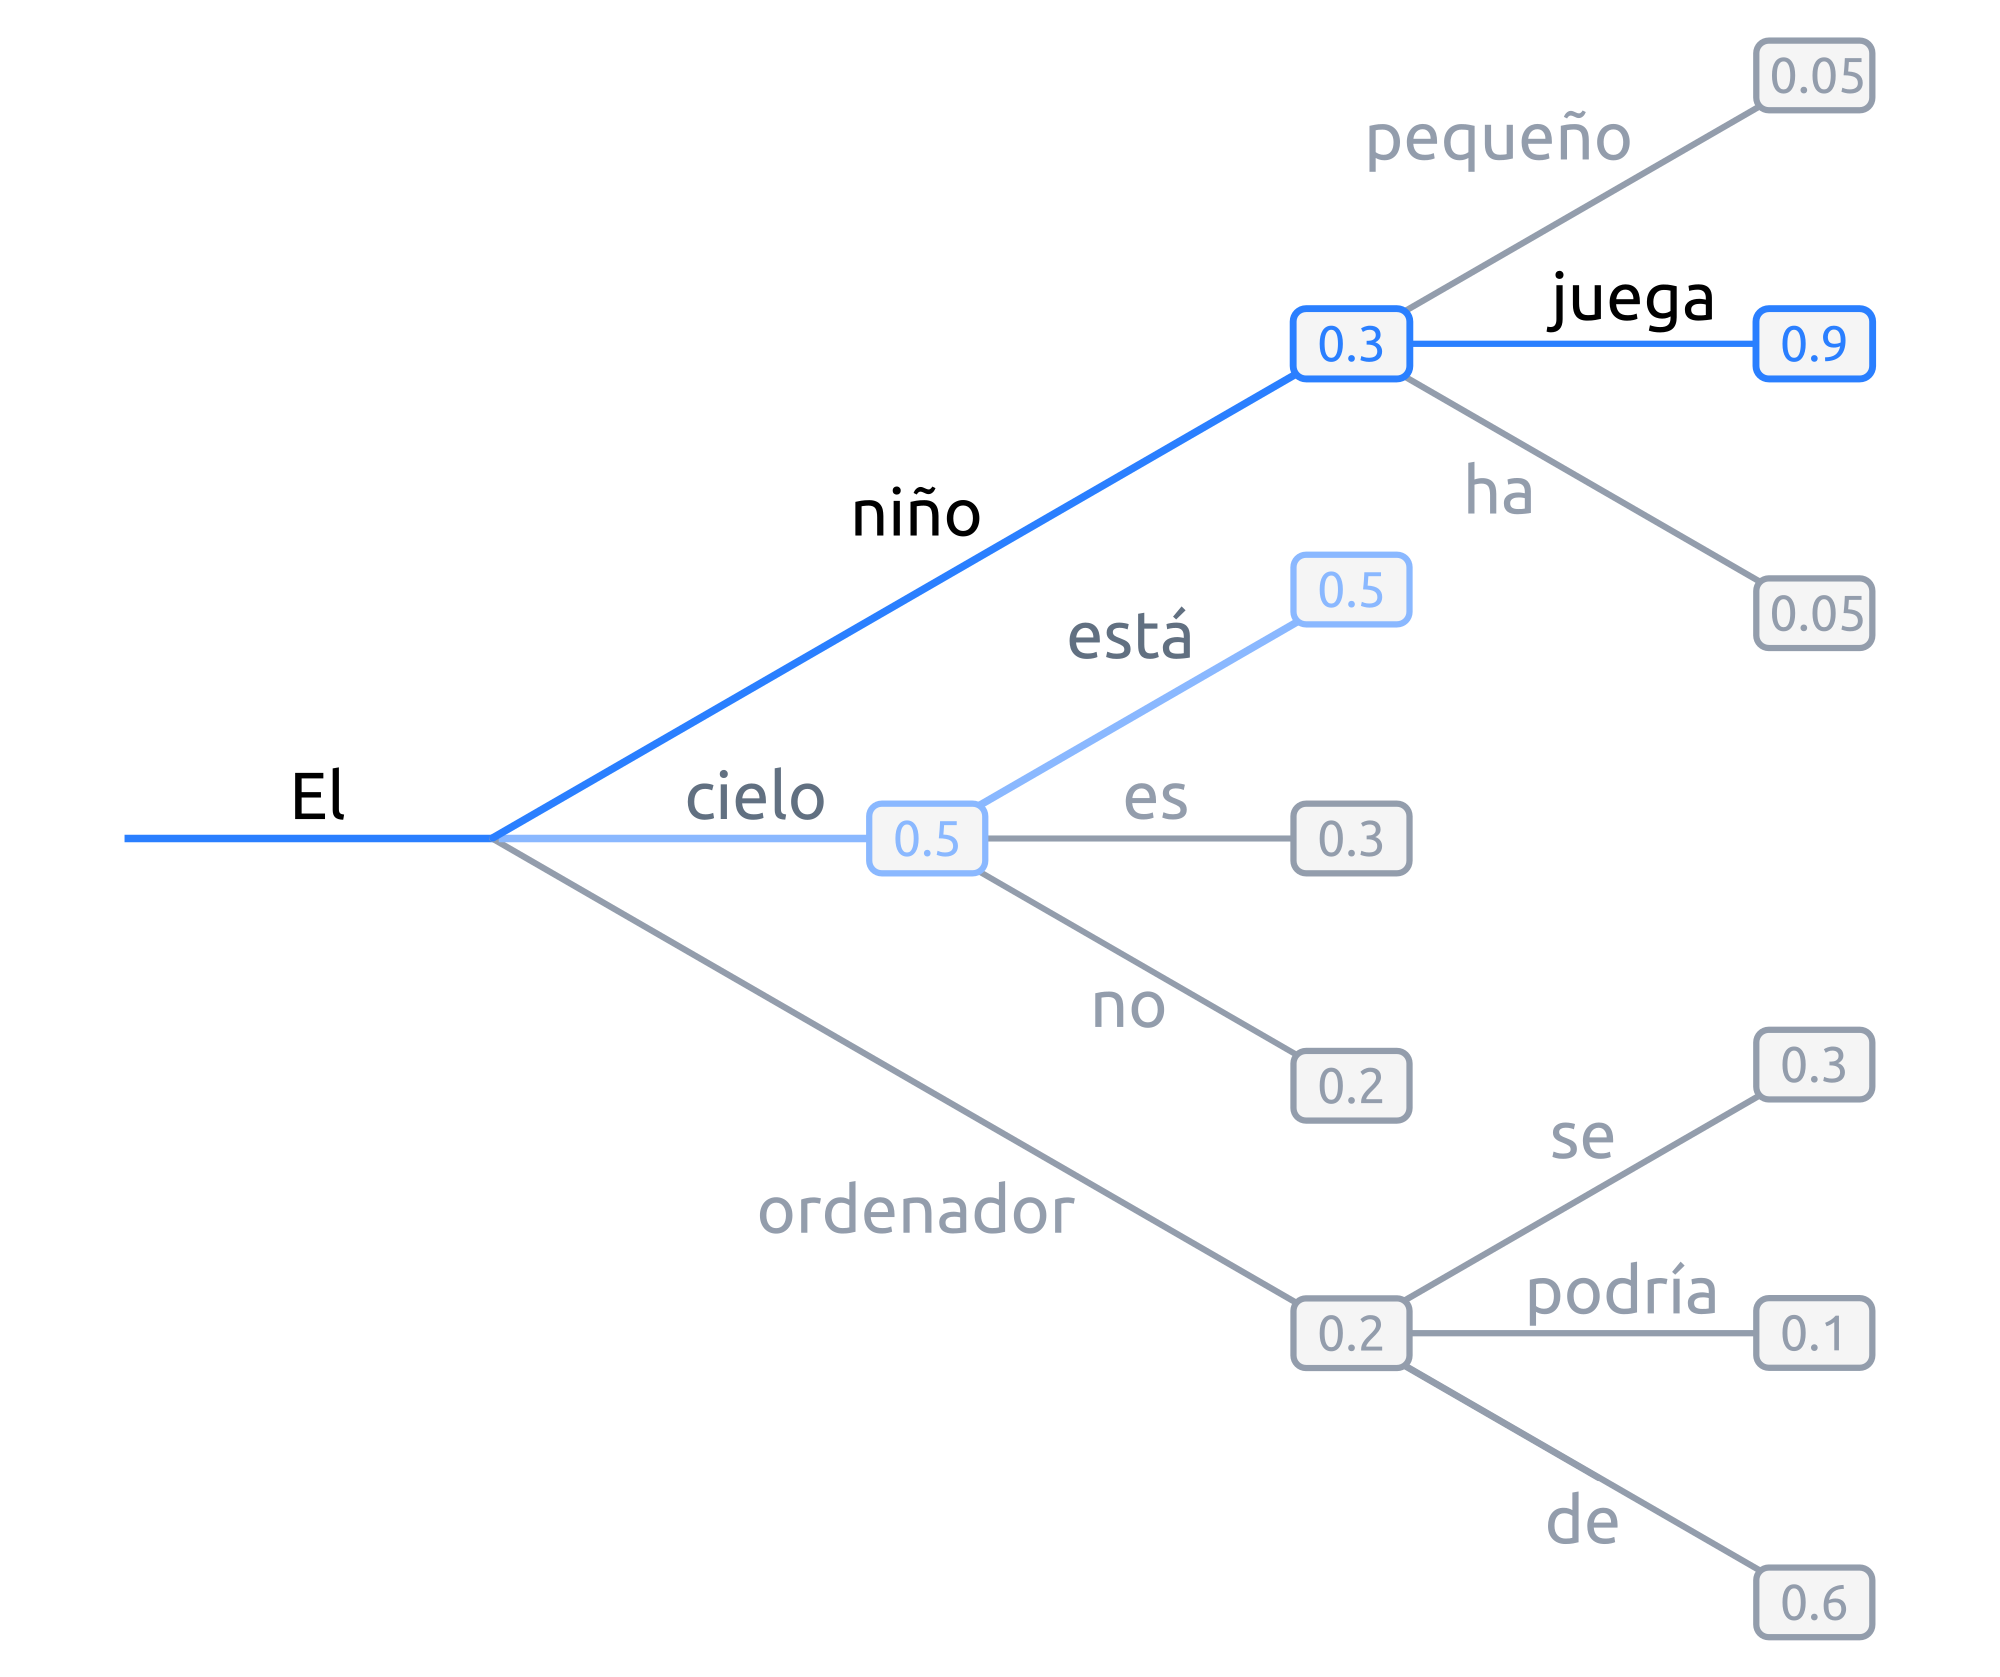
\includegraphics[width=0.7\textwidth]{beam-search}
	\caption{Ejemplo de \emph{beam search} con \texttt{n\_beams = 2}. Durante la búsqueda, se consideran los dos caminos con mayor probabilidad conjunta.}
	\label{fig:beam-search}
\end{figure}

En este ejemplo vemos que, aunque \texttt{``cielo''} presenta mayor probabilidad que \texttt{``niño''}, la secuencia \texttt{``El niño juega''} tiene una mayor probabilidad conjunta ($0.3 \cdot 0.9 = 0.27$) que \texttt{``El cielo está''} ($0.5 \cdot 0.5  = 0.25$), y por tanto será la secuencia elegida.

Este tipo de búsqueda funciona muy bien en tareas en las que la longitud deseada de la secuencia generada se conoce de antemano, como es el caso de la generación de resúmenes, o la traducción automática \cite{murray18, yang18}.

Sin embargo, presenta dos problemas fundamentales:

\vspace*{-\baselineskip}
\begin{itemize}
	\item [\textbullet] De nuevo, aparece el problema de la repetición. Tanto en este caso, como en el de la búsqueda voraz, una estrategia común para evitar dicha repetición, consiste en establecer penalizaciones de \emph{n-gramas} repetidos. Por ejemplo, en el caso de que empleáramos una penalización de 6-gramas, la secuencia \texttt{``El niño juega en el parque''} solo podría aparecer una vez en el texto generado.

	\item [\textbullet] Como se razona en \cite{holtzman20}, el lenguaje humano no sigue una distribución de palabras con mayor probabilidad. Como vemos en la siguiente gráfica, extraída de dicho artículo, la estrategia de \emph{beam search} puede resultar poco espontánea, dando lugar a textos menos <<naturales>>:
	
	\begin{figure}[!h]
		\centering
		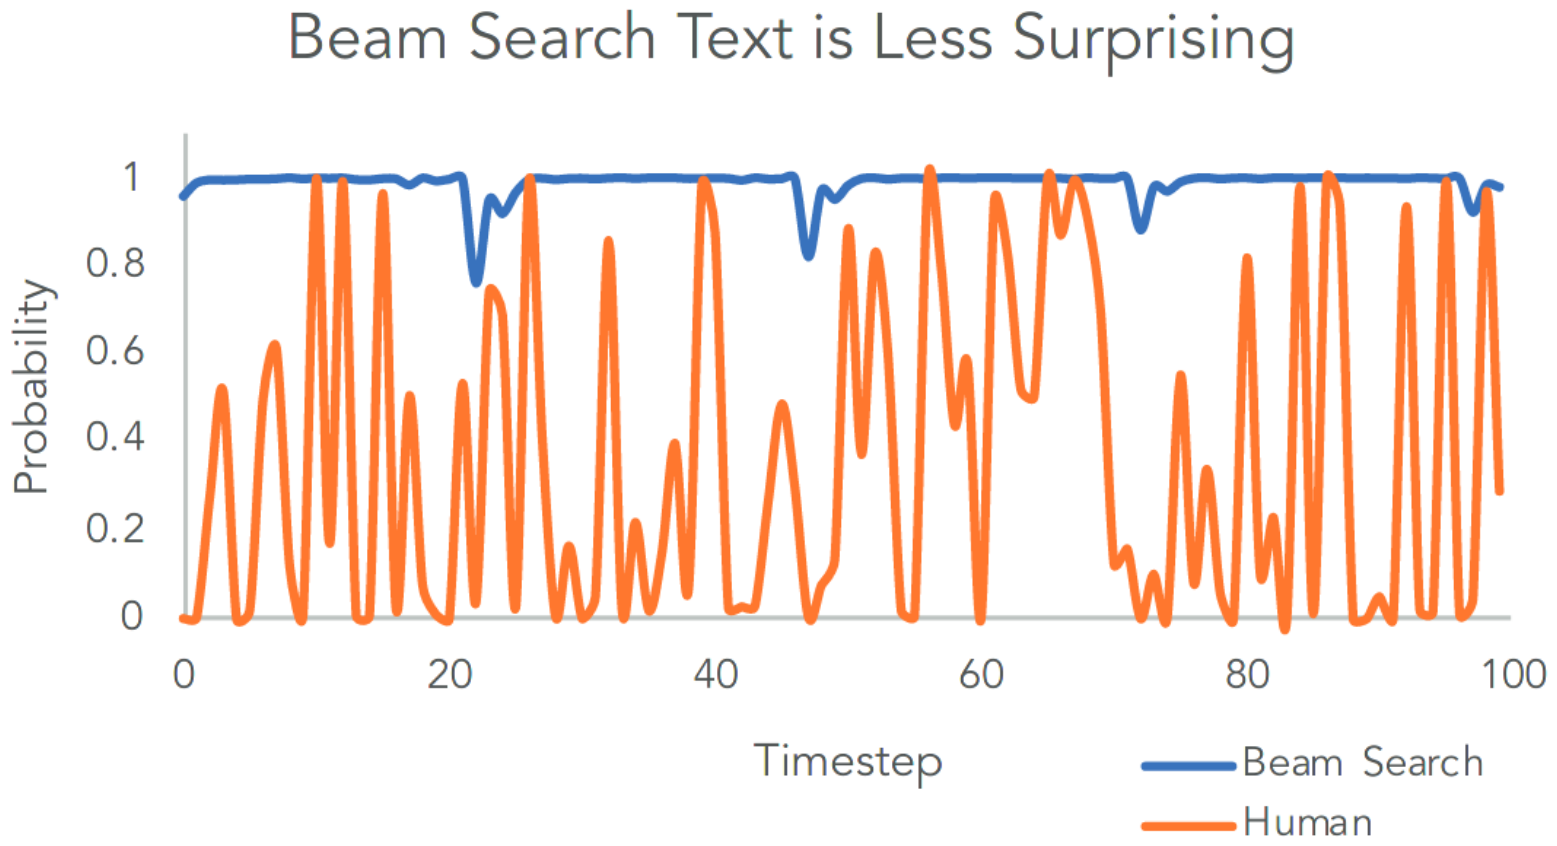
\includegraphics[width=0.7\textwidth]{beam-search-problem}
		\caption{Distribución de probabilidades del lenguaje natural frente a la estrategia de \emph{beam search} \cite{holtzman20}.}
	\end{figure}
\end{itemize}


\bigskip
\noindent
\textbf{Muestreo}

Es su forma más básica, el muestreo simplemente consiste en escoger la siguiente palabra $w_i$ de manera aleatoria en función de la distribución de su probabilidad condicional, es decir:

\[ w_t \sim P(w_t | w_{1:t-1}) \]

De manera gráfica, siguiendo con el ejemplo anterior:

\begin{figure}[!h]
	\centering
	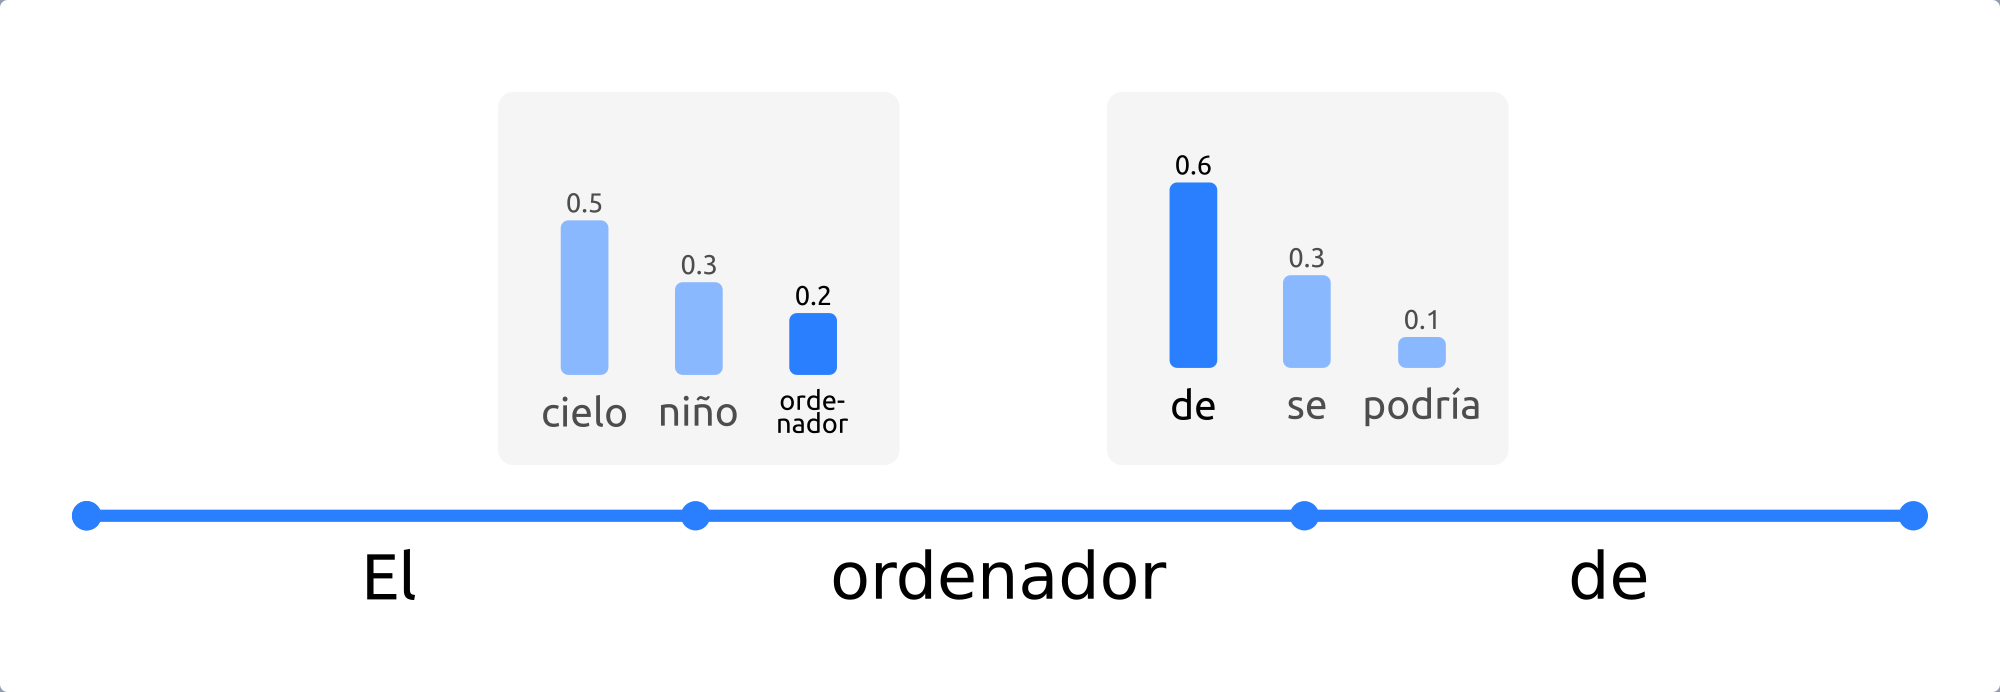
\includegraphics[width=0.8\textwidth]{sampling}
	\caption{Ejemplo de muestreo. En cada paso, se elige una palabra aleatoriamente en función de su probabilidad.}
	\label{fig:muestreo}
\end{figure}

Haciendo uso del muestreo, la generación deja de ser determinista, dando lugar a textos más espontáneos y naturales. Sin embargo, como se estudia en \cite{holtzman20}, esta espontaneidad es a menudo excesiva, dando lugar a textos poco coherentes.

Una solución a este problema consiste en hacer que la distribución $P(w_t|w_{1:t-1})$ sea más acusada, aumentando la verosimilitud (\emph{likelihood}) de palabras con alta probabilidad, y disminuyendo la verosimilitud de palabras con baja probabilidad. Esto se consigue disminuyendo un parámetro denominado \emph{temperatura}\footnote{\hspace{0.06cm}Por motivos de brevedad, no incluiremos una explicación detallada de este parámetro.}. De esta forma, el \hyperref[fig:muestreo]{ejemplo anterior} queda de la siguiente forma:

\begin{figure}[!h]
	\centering
	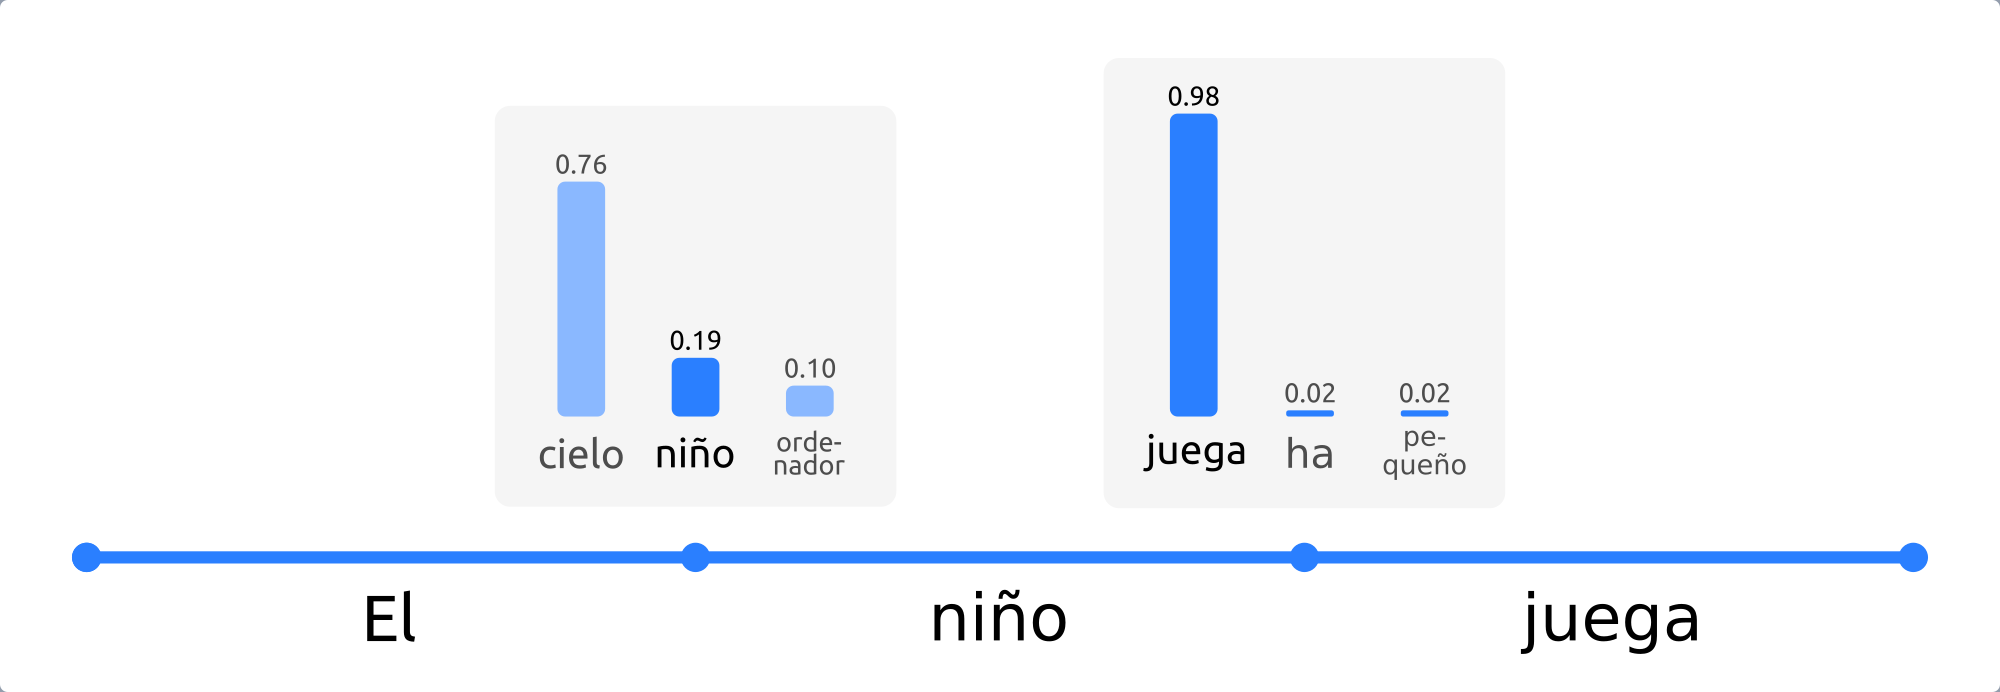
\includegraphics[width=0.8\textwidth]{sampling-temperature}
	\caption{Al decrementar la temperatura, las diferencias en las  probabilidades se hacen más acusadas.}
\end{figure}

Con este ajuste de la temperatura, logramos reducir la aleatoriedad, pero seguimos manteniendo una orientación no determinista.

\newpage

\bigskip
\noindent
\textbf{Muestreo \emph{top-k}}

En ste tipo de muestreo, introducido en \cite{fan18}, en cada paso solo se consideran las \emph{k} palabras con mayor probabilidad (la probabilidad del resto de las palabras será 0).

\begin{figure}[!h]
	\centering
	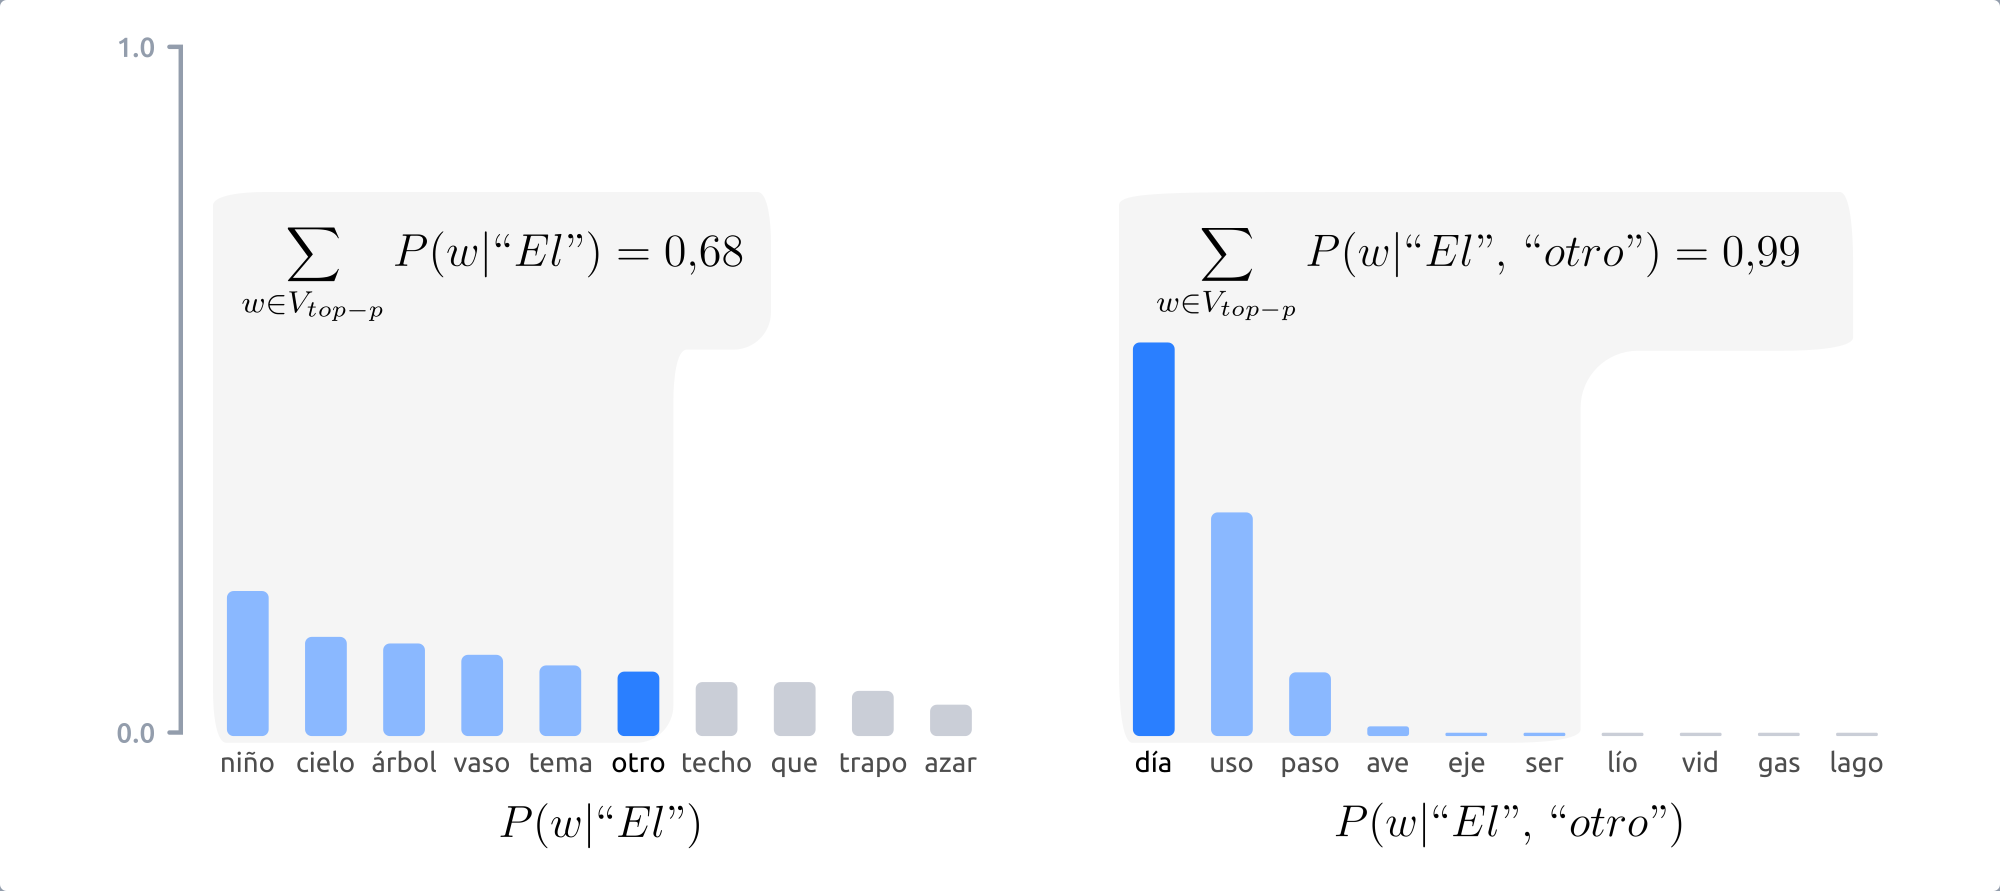
\includegraphics[width=\textwidth]{top-k}
	\caption{Al decrementar la temperatura, las diferencias en las  probabilidades se hacen más acusadas.}
	\label{top-k}
\end{figure}

Tanto la búsqueda voraz como el muestreo visto anteriormente, se pueden como casos particulares del muestreo \emph{top-k}. Si establececemo $k = 1$, estaremos realizando una búsqueda voraz, y si establecemos $k = N$, donde $N$ es la longitud total del vocabulario, estaremos llevando a cabo un muestreo <<puro>>.

Este tipo de muestreo suele producir textos de mayor calidad en situaciones en las que el tamaño de secuencia no está prefijado. Sin embargo, presenta el problema de que el tamaño de \emph{k} se mantiene fijo a lo largo de la generación. Como consecuencia, en pasos en los que la diferencia de probabilidades sea menos acusada, como en el primer paso de la \autoref{top-k}, la espontaneidad del modelo será menor, y en pasos en los que ocurra lo contrario, el modelo será más propenso de escoger palabras que suenen menos naturales, como podría haber ocurrido en el segundo paso de la figura ya mencionada.


\bigskip
\noindent
\textbf{Muestreo \emph{top-p}}

Este tipo de muestreo, en vez de escoger entre un número prefijado de palabras, en cada paso considera el mínimo conjunto de palabras cuyas probabilidades acumuladas superan un cierto valor $p$ \cite{holtzman20}.

\begin{figure}[!h]
	\centering
	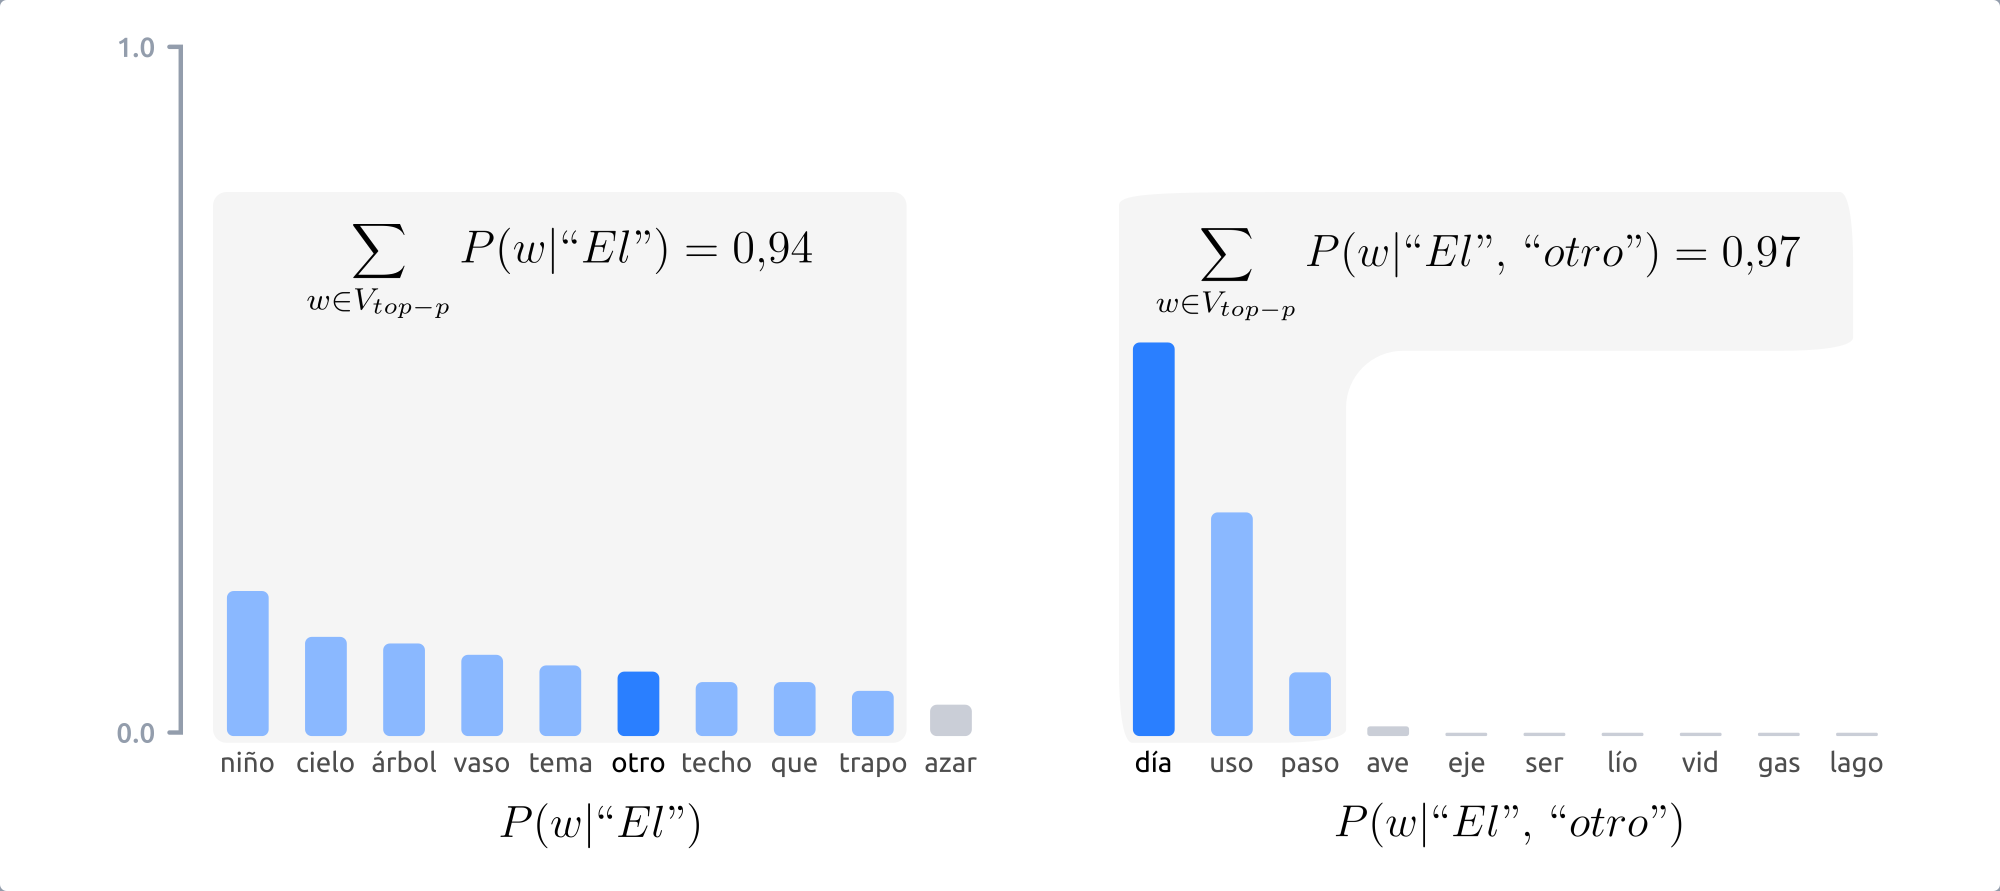
\includegraphics[width=\textwidth]{top-p}
	\caption{Con el muestreo \emph{top-p}, el número de palabras entre las cuales elegir en cada paso varía en función de las probabilidades de las palabras candidatas.}
	\label{top-p}
\end{figure}

La \hyperref[top-p]{figura anterior} muestra como, con $p=0.9$, en el primer paso se consideran 9 palabras, mientras que en el segundo solo 3. De este modo, cuando la siguiente palabra a elegir es menos \emph{predecible}, el modelo puede considerar más candidatas, como en el primer paso del ejemplo mostrado y, en el caso contrario, el número de palabras candidatas se reduce.

Los resultados del muestreo \emph{top-k} u \emph{top-p} son, en la práctica, similares. De hecho, se pueden utilizar de manera conjunta, a fin de evitar la selección de palabras con probabilidades muy bajas, pero manteniendo cierta variación en el número de palabras consideradas.



\section{Post-procesado del texto} \label{sec:postprocesado}

Como veíamos en la \autoref{fig:proceso-resumen}, el resumen producido por el modelo T5, una vez decodificado, se encuentra todo en minúsculas. Por lo demás, el modelo parece hacer un buen trabajo a la hora de generar el texto en lo que a colocación de puntuación y espacios se refiere, luego la principal labor de esta etapa será poner mayúsculas allí donde sean necesarias, lo que en inglés se denomina \emph{truecasing} \cite{lita03}.

Las mayúsculas, tanto en inglés como español, se emplean principalmente en dos ocasiones:

\vspace*{-\baselineskip}
\begin{itemize}
	\item [\textbullet] Al inicio de cada frase. Como veíamos en la sección referente al \hyperref[sec:preprocesado]{pre-procesado} del texto, la separación de un texto en frases no es, por lo general, una tarea trivial. En este caso, podemos reutilizar lo aplicado en dicha etapa. Teniendo el resumen generado dividido en frases, podemos fácilmente poner la primera letra de cada una de ellas en mayúsculas.
	\item [\textbullet] En los nombres propios. En este aspecto, de nuevo vuelve a aparecer el problema del Reconocimiento de Entidades Nombradas (NER). De modo similar a como procedíamos en el pre-procesado, emplearemos un modelo estadístico que realiza la labor de \emph{truecasing}.
\end{itemize}

Tras esta etapa, el resumen está listo para ser entregado al usuario.
	\capitulo{4}{Técnicas y herramientas} \label{chapter:tecnicas}

En este capítulo, se recogen las tecnologías principales empleadas en el desarrollo del proyecto, así como los detalles más relevantes de su implementación.

Para facilitar la organización y comprensión de las mismas, se han separado en tres subsecciones: \hyperref[sec:model]{Modelo}, en la que se detalla el funcionamiento del modelo de generación de lenguaje empleado, \hyperref[sec:backend]{\emph{Backend}}, donde profundizamos en la implementación del servicio escalable en la nube, y \hyperref[sec:frontend]{\emph{Frontend}}, en la que explicamos todo lo referente a la aplicación multiplataforma desarrollada.


\section{Modelo de generación de resúmenes} \label{sec:model}

Como se ha venido mencionando a lo largo de los anteriores capítulos, para la generación de resúmenes se ha elegido el modelo T5 de Google. Más concretamente, utilizamos la implementación \texttt{t5-large} de Hugging Face \cite{t5-hf}, el cual ha sido entrenado con texto en inglés procedente del Colossal Clean Crawled Corpus (C4), y contiene aproximadamente 770 millones de parámetros \cite{hf-pretrained}.

Esta implementación está escrita en Python, lo que nos facilita la integración con el resto de componentes del \emph{backend} de JIZT, también desarrollados en Python.

El modelo \texttt{t5-large} consta, por un lado, del \emph{tokenizer}, encargado de la codificación del texto, y por otro, del modelo en sí, el cual recibe el texto codificado por el \emph{tokenizer}, y genera el resumen a partir de él. Dicho resumen, sigue estando en forma de \emph{tókenes} codificados, por lo que tenemos que hacer uso una vez más del \emph{tokenizer} para proceder a su decodificación. Una vez decodificado, el texto vuelve a contener caracteres legibles.

Tanto el proceso de codificación, como el de generación de resúmenes, se han implementado de forma que se puedan llevar a cabo empleando unidades de procesamiento gráfico (GPU). No obstante, en nuestro caso y por el momento, ambos procesos se ejecutan en unidades centrales de procesamiento (CPU), debido a limitaciones económicas\footnote{\, Cabe recordar que los modelos se ejecutan en <<la nube>>. Contratar equipos que dispongan de GPU aumentaría notablemente los costes.}. Esto explica en parte los \hyperref[table:comparativa]{tiempos de resumen obtenidos}, los cuales pueden resultar algo dilatados con textos muy largos.

Un último aspecto a destacar es que a la hora de generar los resúmenes, se pueden especificar los parámetros concretos con los que realizar dicha generación, permitiéndonos hacer uso de las diferentes estrategias vistas en la \autoref{subsec:estrategias-gen}.

\section{\emph{Backend} --- Plataforma escalable en la nube} \label{sec:backend}

En la \autoref{fig:overview-arch} se recoge una visión general de la arquitectura que conforma el \emph{backend} de JIZT, y que posibilita la implementación en la nube de las diferentes etapas en la generación de resúmenes descritas en el capítulo de \hyperref[chapter:conceptos]{Conceptos teóricos}.

\begin{figure}[!h]
	\centering
	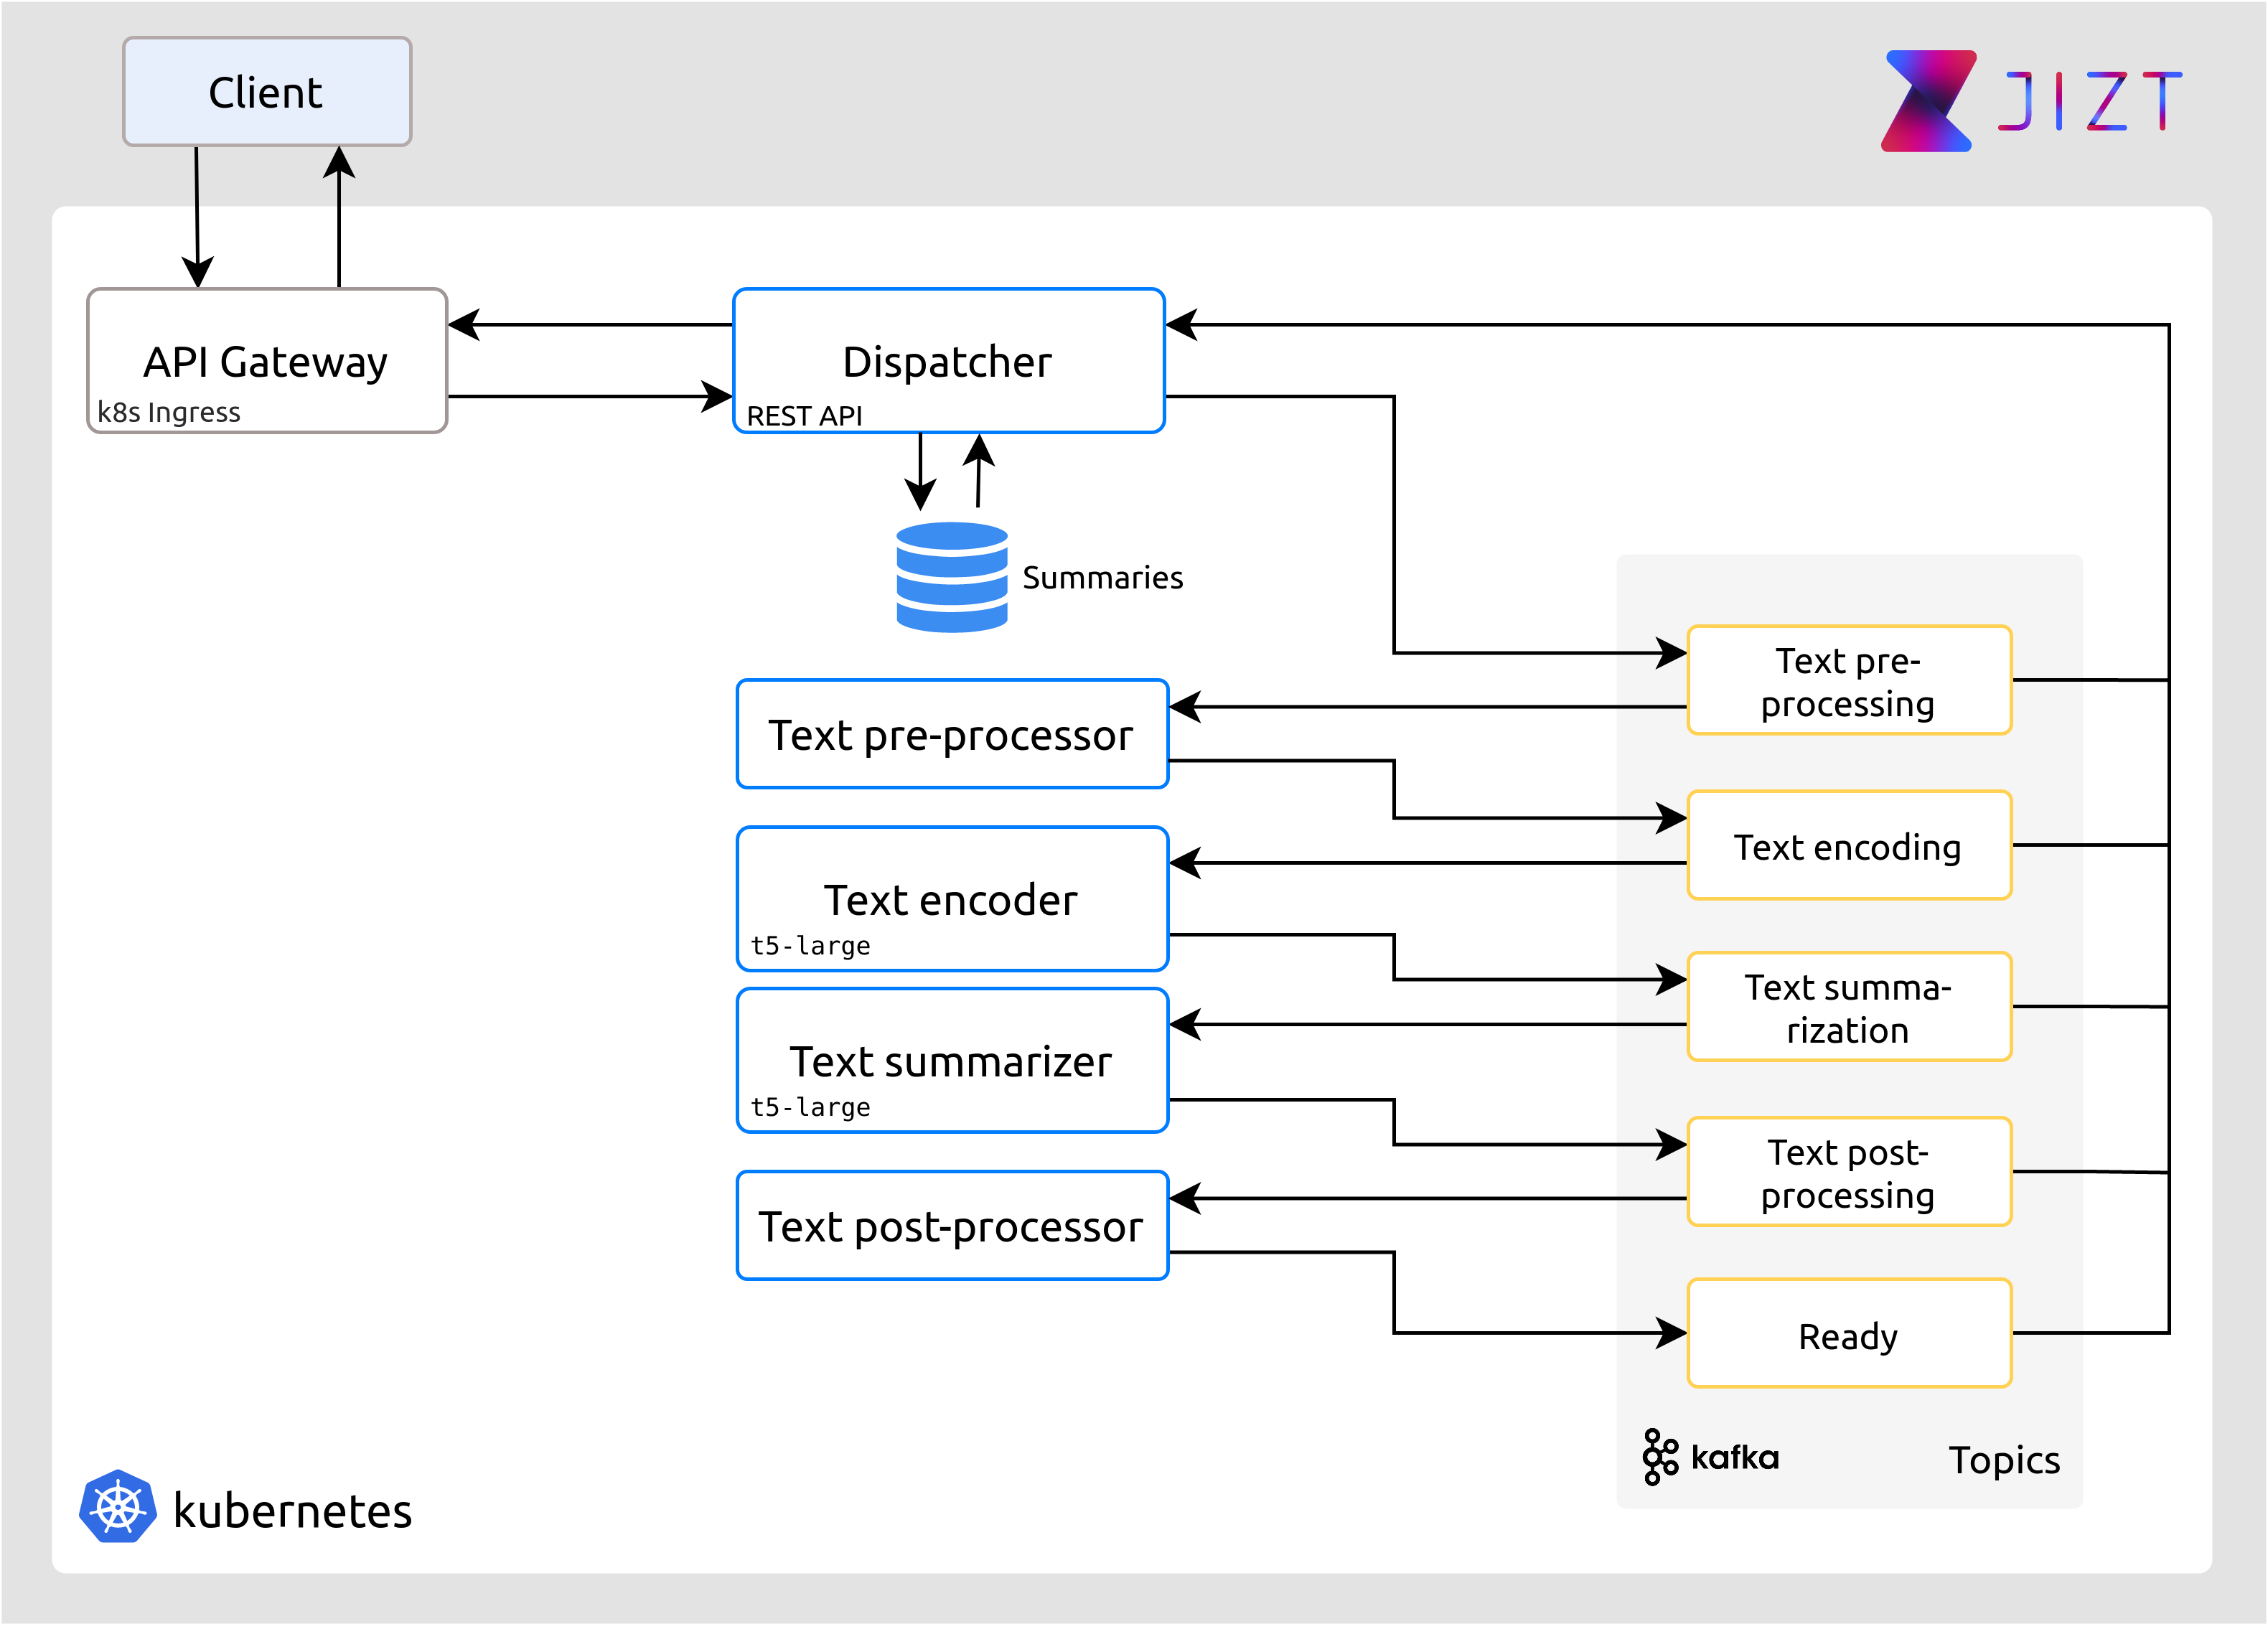
\includegraphics[width=\textwidth]{overview-arch}
	\caption[Vista general de la arquitectura del \emph{backend}.]{Vista general de la arquitectura del \emph{backend}. Los rectángulos en azul se corresponden con los microservicios de JIZT, encapsulados en contenedores Docker. Los rectángulos en amarillo, representan los \emph{topics} de Kafka, explicados posteriormente.}
	\label{fig:overview-arch}
\end{figure}

En esta arquitectura, existen diferentes tecnologías, cada una encargada de realizar una tarea específica, pero a su vez integrándose con el resto. A grandes rasgos, y sin ser necesario que el lector comprenda con exactitud todos los términos por ahora, presentemos brevemente cuáles son las tecnologías empleadas.

En primer lugar, cada microservicio se encapsula en un contenedor Docker. De esta forma, además de modularizar cada microservicio, podemos aumentar el número de réplicas de cada uno de ellos, permitiendo el escalado de la arquitectura.

Por su parte, Kubernetes se encarga de la \emph{orquestración} de los microservicios, ocupándose de aspectos como la replicación, configuración de red y almacenamiento, gestión de los recursos del sistema, etc. El despliegue de los componentes que componen Kubernetes se simplifica gracias al uso de otra herramienta, Helm.

Otra de las tecnologías usadas, Apache Kafka, permite la comunicación entre los diferentes microservicios mediante eventos.

El despliegue de la base de datos PostgreSQL en Kubernetes encargada de almacenar los resúmenes generados, corre a cargo del Operador de PostgreSQL de Crunchy.

Por último, la API REST se implementa a través de un popular \emph{framework} para Python, llamado Flask.

Expliquemos, ahora sí, de forma detallada cómo funciona cada una de estas tecnologías.

\subsection{Docker}

Docker nos permite encapsular nuestros microservicios en contenedores. De este modo, gracias a Kubernetes, podemos crear réplicas de cada microservicio, haciendo posible el escalado de nuestro sistema.

A diferencia de las máquinas virtuales, en las cuales el sistema operativo subyacente se comparte a través del hipervisor, cada contenedor Docker ejecuta su propio sistema operativo, como podemos ver en la siguiente figura:

\begin{figure}[!h]
	\centering
	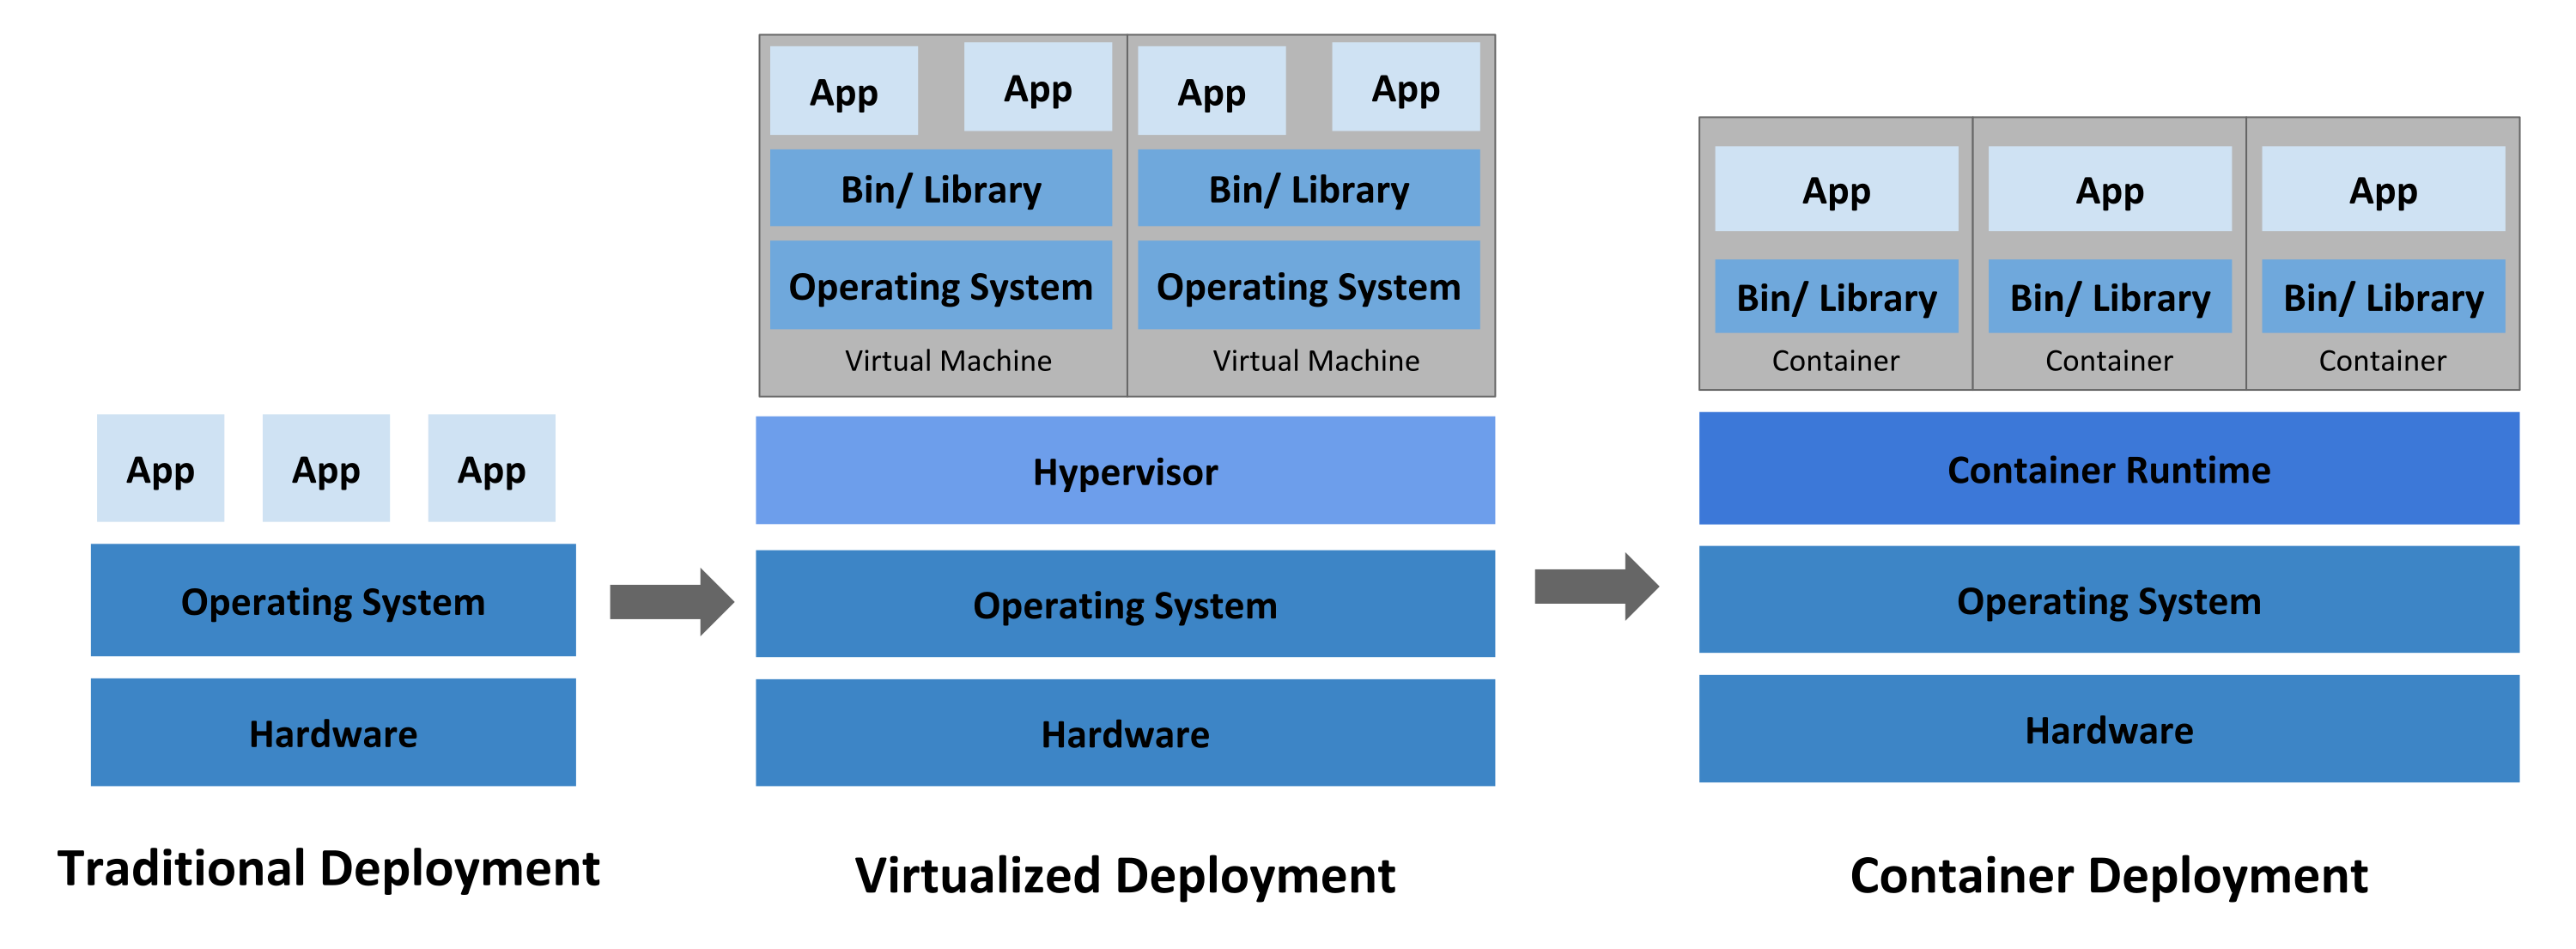
\includegraphics[width=\textwidth]{docker}
	\caption[Diferentes enfoques en el despliegue de sistemas.]{Comparativa de los diferentes enfoques en el despliegue de sistemas: desarrollo tradicional, desarrollo virtualizado, y desarrollo con contenedores \cite{kubernetes}.}
	\label{fig:vm-container}
\end{figure}

Otra ventaja de Docker es que nos permite distribuir la implementación de nuestros microservicios a través imágenes, por lo que un desarrollador que solo quisiera hacer uso de uno de los microservicios, podría hacerlo de manera sencilla.

\subsection{Kubernetes}

El \emph{backend} sigue una arquitectura de microservicios \cite{newman15}, de forma que cada una de las etapas (pre-procesado, codificación, generación del resumen y post-procesado), está confinada en un contenedor Docker \cite{docker}, conformando un microservicio. Adicionalmente, existe un microservicio más, el \emph{Dispatcher}, el cual lleva a cabo las siguientes tareas:

\vspace{-0.5cm}
\begin{itemize}
	\item [\textbullet] Implementa una API REST que permite a los clientes solicitar resúmenes.
	\item [\textbullet] Gestiona una base de datos en la que se almacenan los resúmenes generados.
	\item [\textbullet] Redirige las peticiones de los clientes al microservicio apropiado. Por ahora, todas las peticiones se redirigen hacia el pre-procesador de textos, pero en un futuro podría existir otro microservicio que se encargara, por ejemplo, de extraer el texto de un documento PDF o de una página \emph{web}. En estos casos, el \emph{Dispatcher} se encargaría de redirigirlo hacia el microservicio correspondiente.
\end{itemize}

Kubernetes es una plataforma \emph{open-source} destinada a la gestión de servicios y cargas de trabajo en contenedores, facilitando su automatización en cuanto a aspectos como el escalado, gestión de red y recursos, monitorización, etc. \cite{kubernetes}.

Kubernetes comprende numerosos componentes, entre los cuales, los más relevantes para nuestro proyecto son:

\vspace{-0.5cm}
\begin{itemize}
	\item [\textbullet] \emph{Pod}: es la unidad de computación básica en Kubernetes. Un \emph{Pod} puede ejecutar uno o varios contenedores intrínsecamente relacionados (compartirán almacenamiento, red, recursos, etc.). 
	\item [\textbullet] \emph{Deployment}: los \emph{deployments} se pueden ver como <<plantillas>> o <<moldes>> que contienen los detalles específicos para crear \emph{pods} de un determinado tipo. Por ejemplo, en el caso del mencionado \emph{Dispatcher}, dispondremos de un \emph{deployment} que indicará cómo se deben crear los \emph{pods} para este servicio, todos ellos idénticos. Estos \emph{pods} a su vez, contendrán todos la misma imagen Docker que implementará la lógica del servicio.
	\item [\textbullet] \emph{Service}: cada \emph{pod} dispone de una dirección IP propia. Sin embargo, los \emph{pods} tienen un ciclo de vida \emph{efímero}, dado que están concebidos para ser reemplazados dinámicamente si se producen errores, actualizaciones, etc. Por tanto, no podemos basar la configuración de red en las IPs específicas de los \emph{pods}, ya que estás son susceptibles de cambiar a lo largo del tiempo, según los \emph{pods} vayan siendo reemplazados. Los \emph{services} nos permiten asociar una IP fija y persistente a un conjunto concreto de \emph{pods}. A la hora de realizar una conexión con dicha IP, Kubernetes se encarga de remitir los datos al \emph{pod} que esté menos ocupado en ese instante, realizando por tanto un balance de carga de forma automática.
	
	\item [\textbullet] \emph{PersistentVolume}: al igual que en el caso de las IPs, los datos almacenados localmente en un \emph{pod} desaparecerán cuando este sea reemplazado. Los \emph{PersistentVolumes} nos proporcionan la capacidad de almacenar datos de manera persistente, independientemente del ciclo de vida de los \emph{pods}. Nosotros, utilizamos este componente para almacenar los modelos de generación de resúmenes, ya que ocupan alrededor de 5 GB, de forma que los \emph{pods} correspondientes a la codificación de texto y generación del resumen consumen los modelos desde una única fuente de datos, el \emph{PersistentVolume}. Incluir los modelos dentro de los propios \emph{pods} sería contraproducente ya que (a) todos los \emph{pods} van a hacer uso de los mismos modelos, y (b) los modelos tienen un tamaño del orden de \emph{gigas}, por lo que si quisiéramos crear varios \emph{pods}, la demanda de almacenamiento crecería rápida e innecesariamente.
\end{itemize}

La \autoref{fig:k8s-components} pretende facilitar la comprensión de los diferentes componentes de manera más visual. Como podemos ver en dicha figura, existen \emph{n} \emph{pods}, todos ellos replicas de un mismo \emph{deployment} y, por tanto, ejecutando los mismos contenedores, pero cada uno de ellos con una dirección IP propia. El \emph{service} permite acceder a los diferentes \emph{pods} a través de una única IP estática. Por último, todos los \emph{pods} consumen un mismo \emph{PersistentVolume} que, por ejemplo, podría contener los modelos ya mencionados.

\begin{figure}[!h]
	\centering
	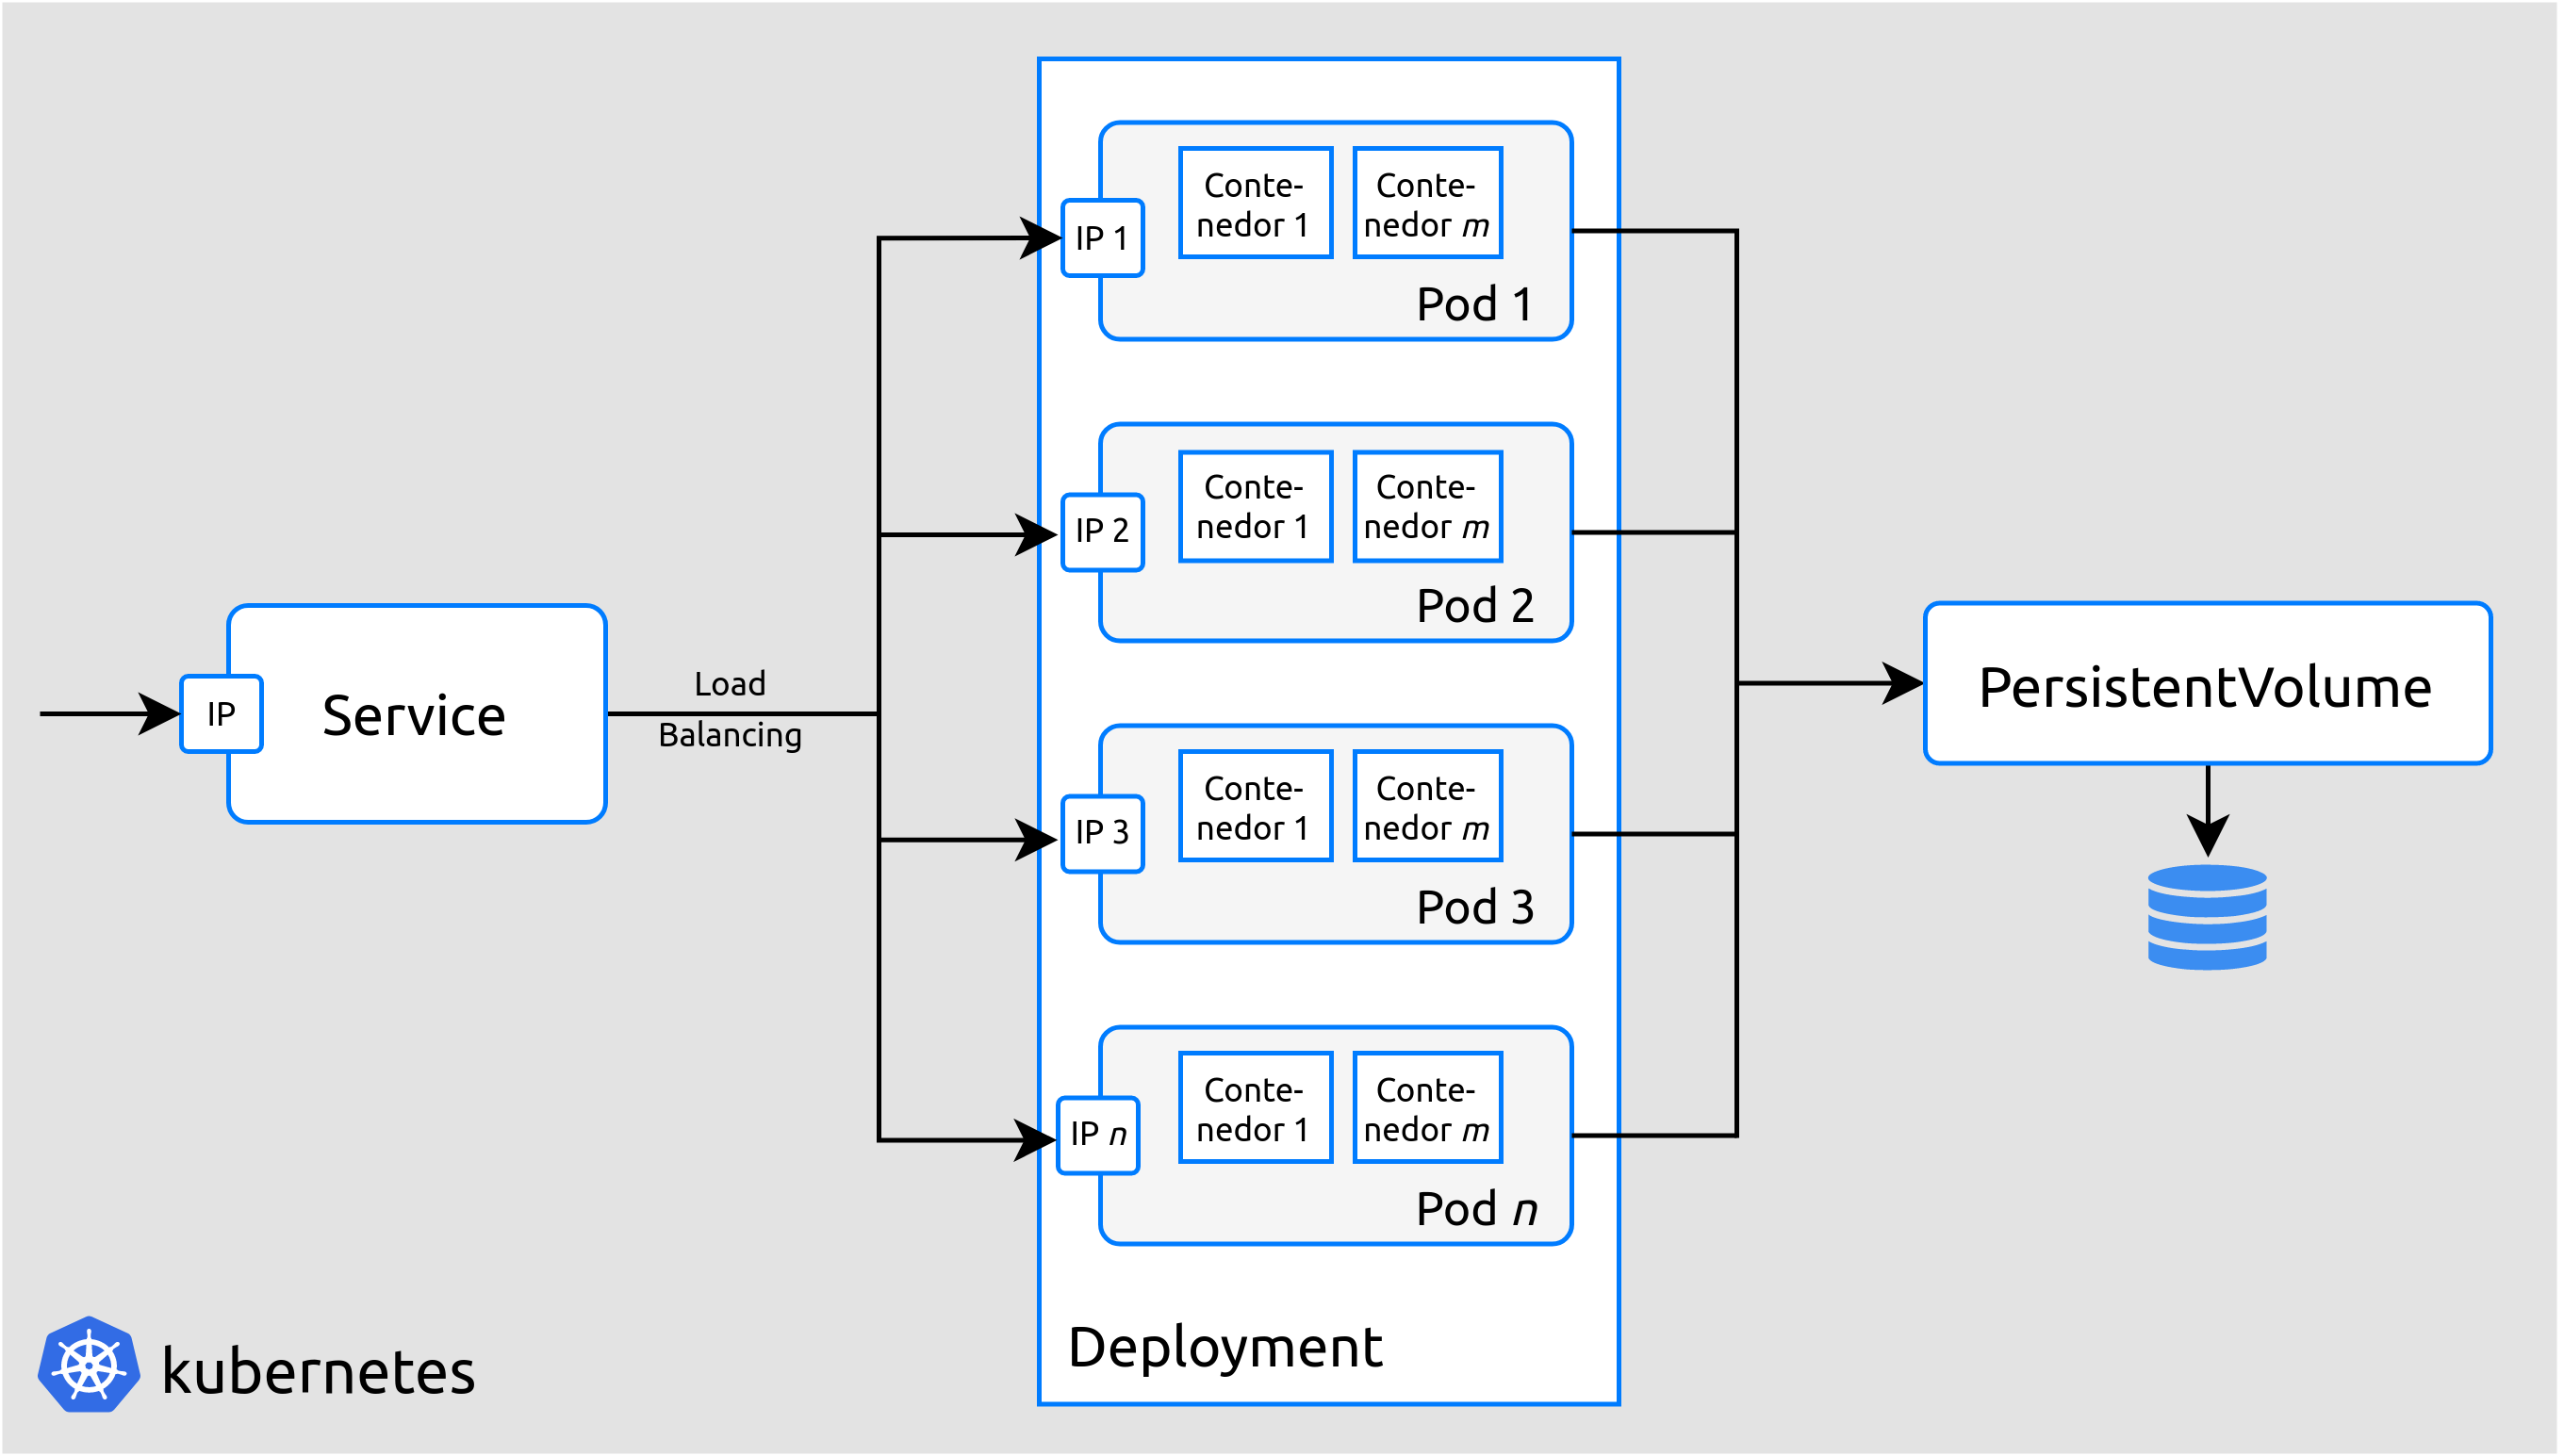
\includegraphics[width=\textwidth]{kubernetes-components}
	\caption{Componentes principales de Kubernetes.}
	\label{fig:k8s-components}
\end{figure}

De este modo, podemos escalar (o actualizar) cada uno de los microservicios de forma dinámica y sin periodos de inactividad (\emph{downtime}). De hecho, Kubernetes permite configurar dicho escalado de manera automática. Así, en momentos en los que la carga de trabajo sea mayor, Kubernetes se encargará de crear \emph{pods} adicionales para responder ante dicha carga y, una vez esta desaparezca, los volverá a eliminar. Al habilitar esta opción, es muy recomendable configurar el número máximo de \emph{pods} que se podrán crear, a fin de evitar un escalado descontrolado en momentos de carga extrema (en cualquier caso, Kubernetes detendría la creación de \emph{pods} tan pronto como se consumieran los recursos disponibles del sistema \cite{k8s-scheduling}).

Existe un último componente de Kubernetes del que hacemos uso, llamado Ingress. Este componente implementa una API \emph{Gateway}, enrutando las peticiones API de los clientes hacia el microservicio correspondiente \cite{api-gateway}. Por ahora, la API REST que hemos implementado solo dispone de rutas relacionadas a la generación de resúmenes, pero en un futuro, cuando se implementen otras tareas de NLP, existirán otros \emph{endpoints} para dichas tareas. Ingress se encargará entonces de, en función de a qué \emph{endpoint} se esté realizando la petición, redirigirla al microservicio correspondiente.

\begin{figure}[!h]
	\centering
	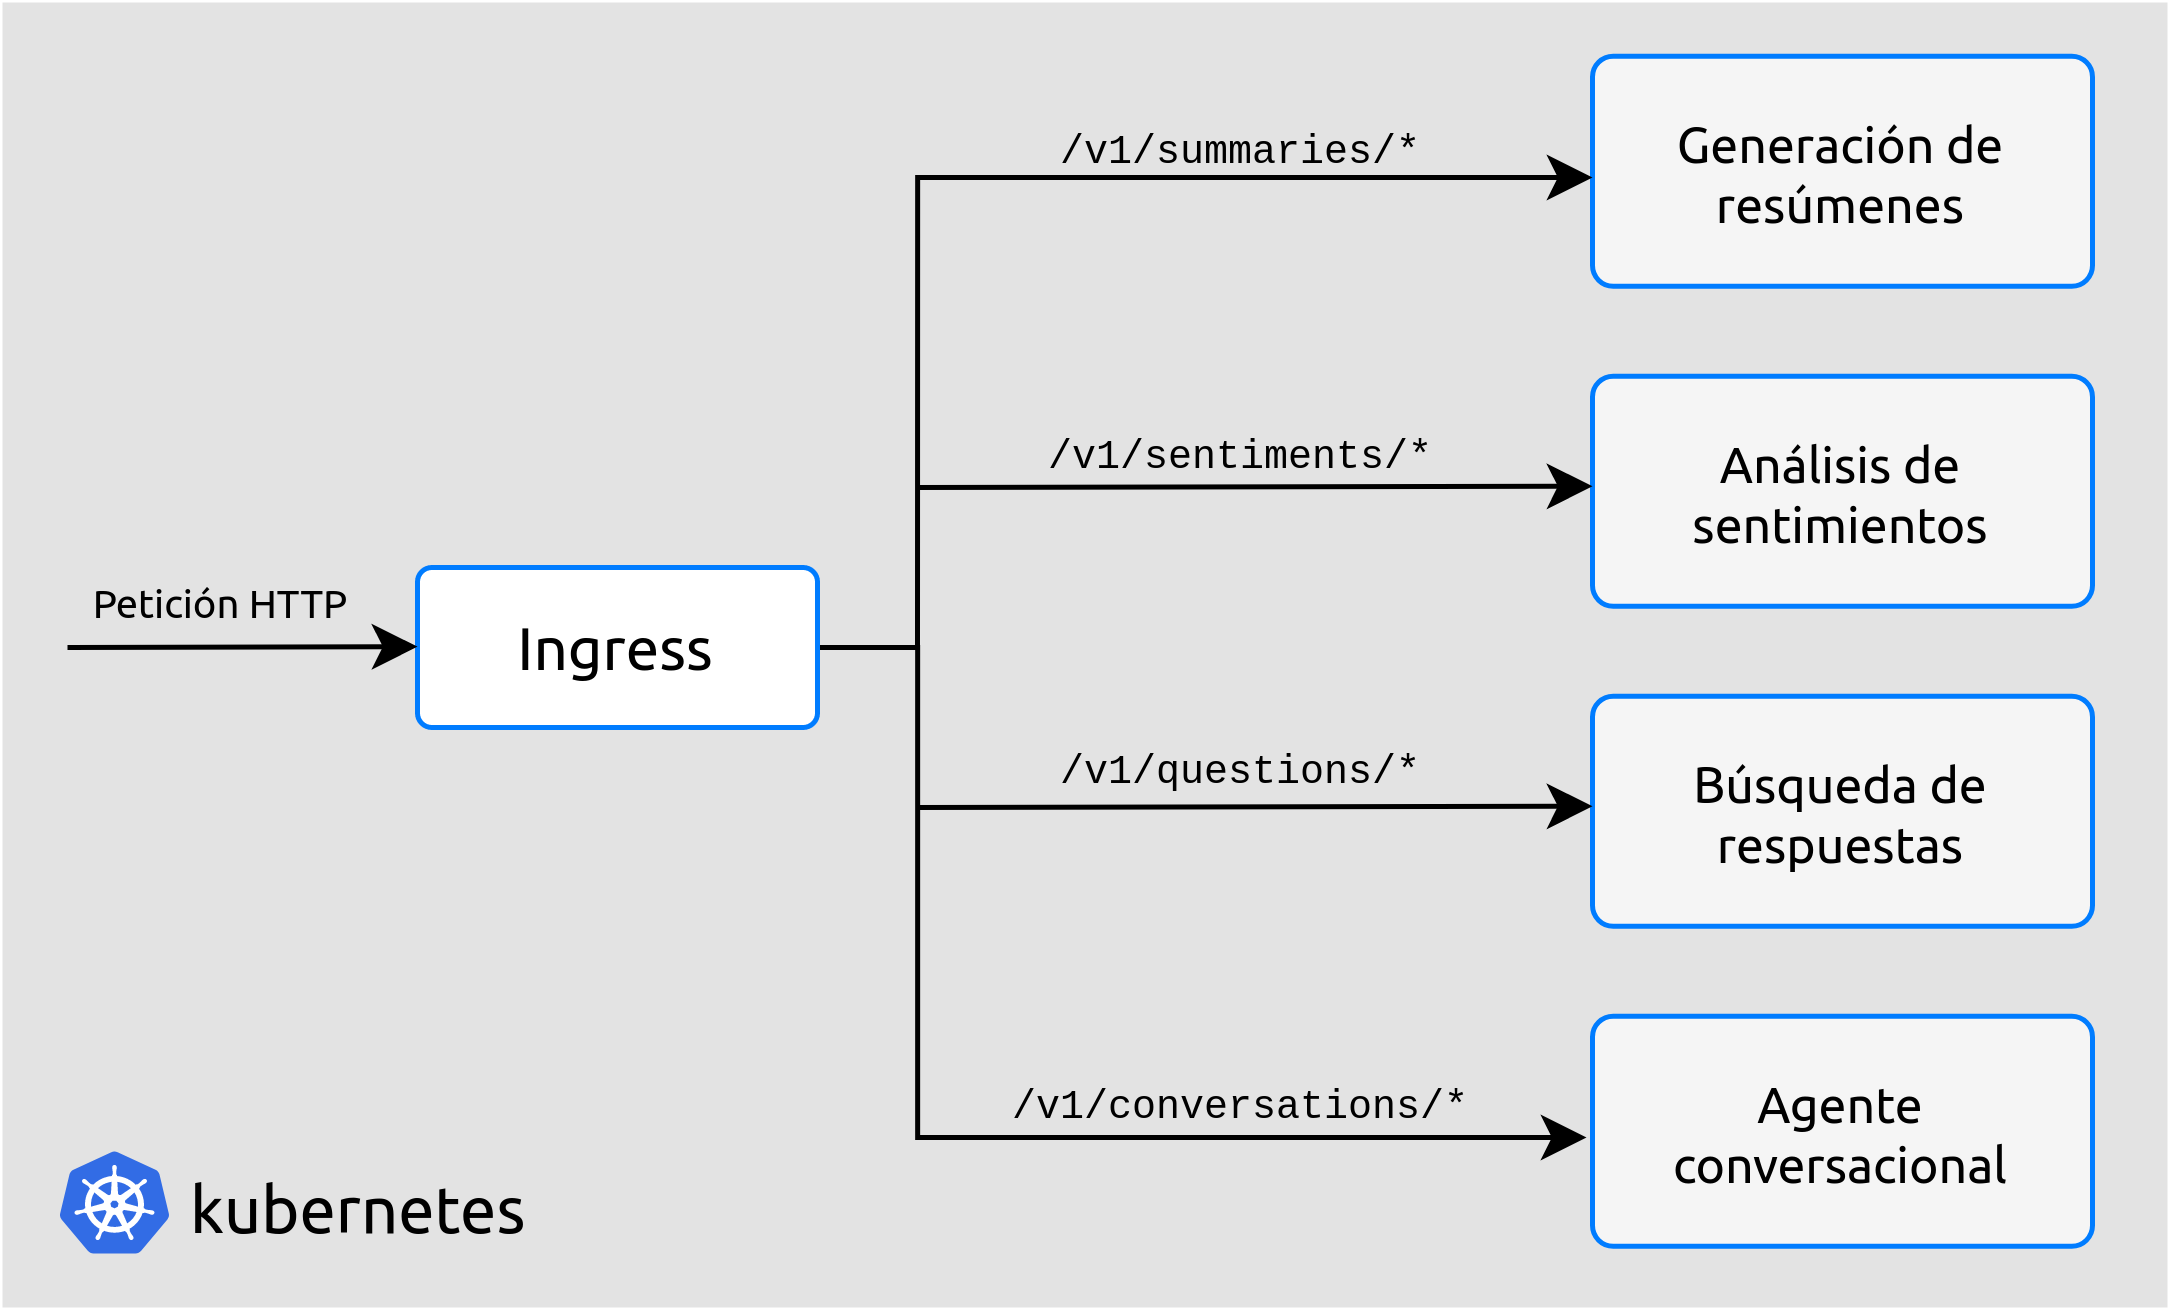
\includegraphics[width=0.9\textwidth]{kubernetes-ingress}
	\caption[Ejemplo de uso de Ingress con diferentes rutas.]{Ejemplo de un hipotético uso de Ingress con diferentes rutas.}
	\label{fig:k8s-ingress}
\end{figure}


\subsection{Kafka y Strimzi} \label{subsec:kafka}

Uno de los principales aspectos a considerar a la hora de implementar una arquitectura de microservicios, reside en la estrategia que se va seguir para permitir la comunicación entre los diferentes microservicios.

Dicha comunicación puede llevarse a cabo de forma síncrona, por ejemplo a través de peticiones HTTP, o asíncrona, con tecnologías como Apache Kafka \cite{microsoft-microsvcs}.

En nuestro caso la comunicación síncrona quedó rápidamente descartada, dado que la generación de resúmenes presenta tiempos de latencia que pueden ser elevados (del orden de segundos o incluso minutos). Decidimos, por tanto, adoptar la segunda opción.

Apache Kafka nació internamente en LinkedIn, aunque actualmente es \emph{open-source} y su desarrollo corre a cargo de la Apache Software Foundation ~\cite{wiki-kafka}.

Kafka permite el intercambio asíncrono de mensajes entre productores y consumidores. En esencia, su funcionamiento es conceptualmente sencillo y está alineado con tecnologías más tradicionales: los consumidores se subscriben a un tema (\emph{topic}), a los que los productores envían sus mensajes. La consumición de dichos mensajes es asíncrona.

La novedad de Kafka reside, entre otras cosas, en su gran capacidad de escalado, pudiendo soportar billones de mensajes al día; su funcionamiento distribuido, de manera que puede operar fácilmente a lo largo de diferentes zonas geográficas; su gran fiabilidad en entornos críticos, en los que la pérdida de un solo mensaje es inadmisible; o su tolerancia frente a fallos \cite{apache-kafka}.

Todas estas demandas no suponen, sin embargo, que Kafka no se pueda aplicar de igual modo a entornos más reducidos, como es el nuestro. Además, gracias a Strimzi, otro proyecto también \emph{open-source}, el despliegue de Kafka en Kubernetes se simplifica en gran medida.

Si volvemos a observar la figura que ilustra la arquitectura general del \emph{backend} (\autoref{fig:overview-arch-2}), podemos ver que JIZT dispone de cinco \emph{topics}, los cuales se corresponden con cada una de las etapas en la generación resúmenes.

\begin{figure}[!h]
	\centering
	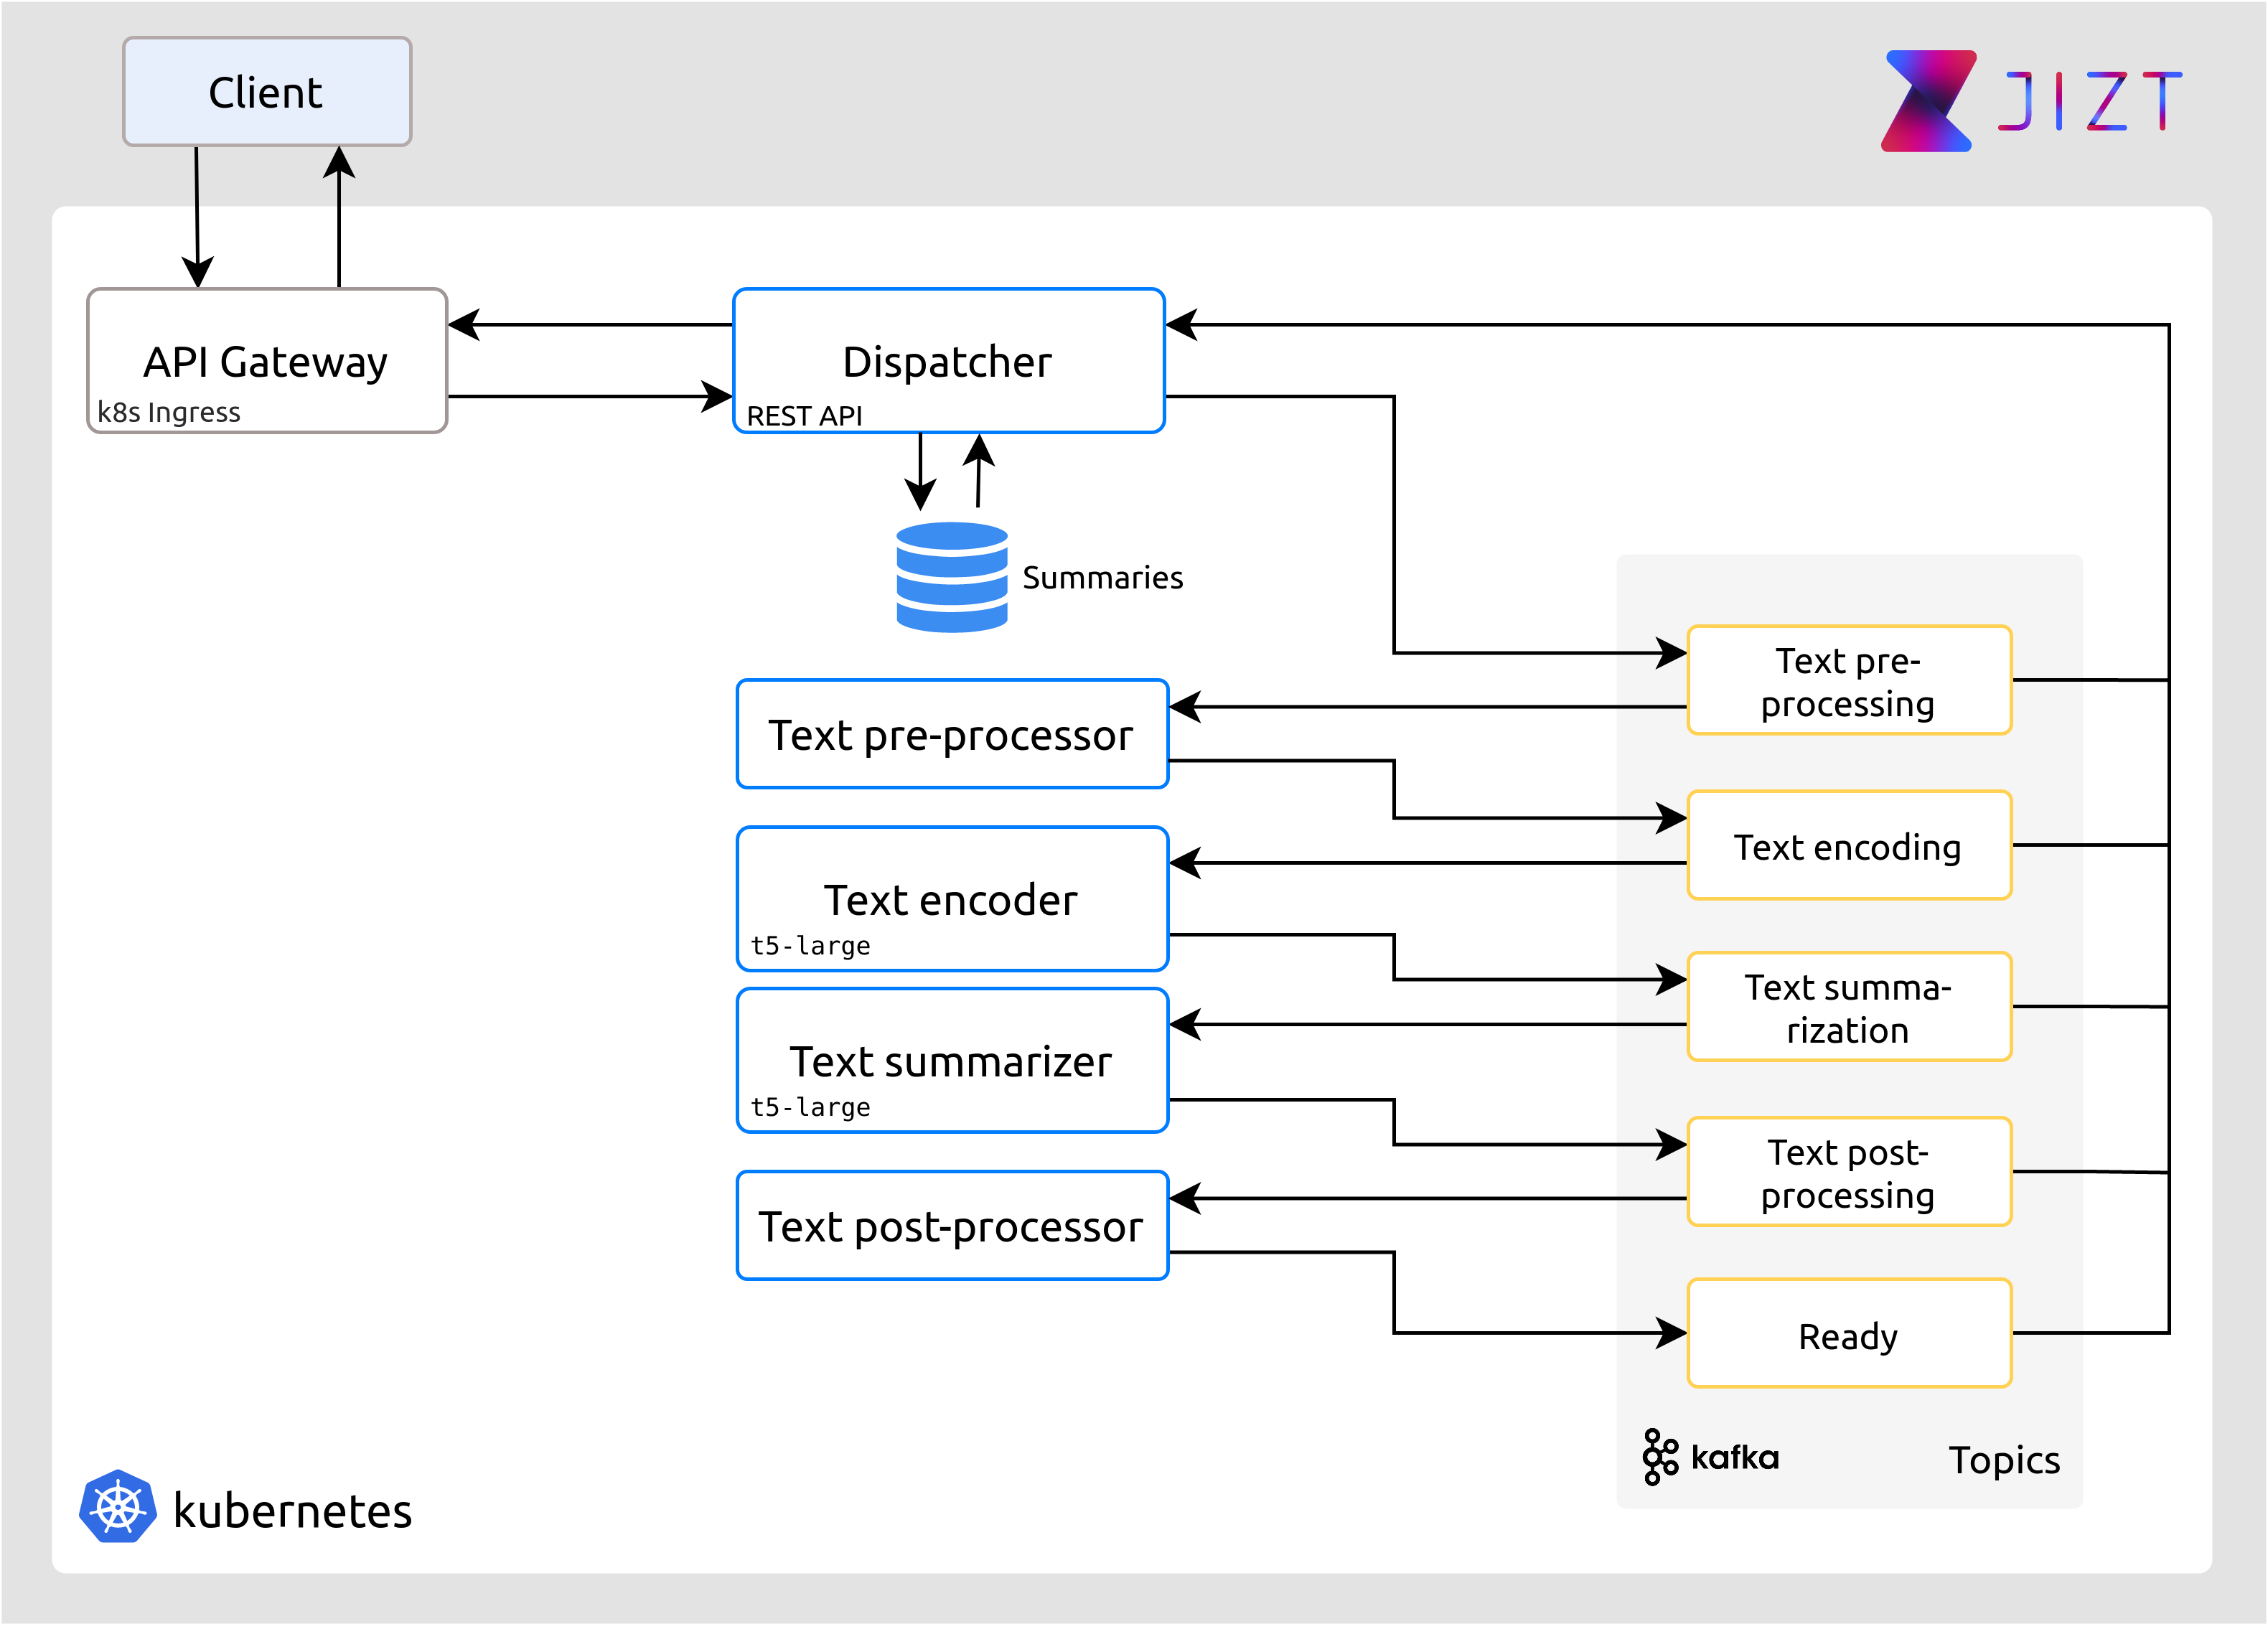
\includegraphics[width=\textwidth]{overview-arch}
	\caption{Vista general de la arquitectura del \emph{backend}.}
	\label{fig:overview-arch-2}
\end{figure}

Con esta figura en mente, el proceso completo que se sigue es el siguiente:

\begin{enumerate}
	\item El cliente realiza una petición HTTP POST solicitando un nuevo resumen. Para ello, debe incluir en el cuerpo el texto a resumir, y de manera opcional los parámetros del resumen a generar.
	
	\item Ingress (API \emph{Gateway}) comprueba que dicha petición se está haciendo a un \emph{endpoint} válido, y en ese caso la redirige hacia el \emph{Dispatcher}. En caso contrario devolverá un error HTTP 404.
	
	\item El \emph{Dispatcher} realiza una serie de comprobaciones:
	\begin{enumerate}
		\item Si la petición no contiene ningún texto, se devuelve un error. En el caso de los parámetros, si son incorrectos o inexistentes, se ignoran y se utilizan valores por defecto.
		
		\item Se consulta en la base de datos si ya existe un resumen generado para ese texto con esos mismos parámetros. En ese caso, lo devuelve directamente, sin generar de nuevo el resumen.
		
		\item En caso contrario, produce un mensaje al \emph{topic} del pre-procesador de textos, conteniendo el texto y los parámetros del resumen.
	\end{enumerate}

	\item El pre-procesador está constantemente comprobando si existen mensajes nuevos en su \emph{topic}. En ese caso los consume, realiza las tareas de pre-procesado, y produce el resultado en el \emph{topic} del codificador.
	
	\item Este proceso continua de forma análoga hasta llegar al post-procesador, el cual produce el resumen final al \emph{topic} <<Listo>> (\emph{Ready}). El \emph{Dispatcher}, en ese momento, consume el mensaje, actualiza la base de datos, y proporciona el resumen al cliente.
\end{enumerate}

En dicha figura, vemos también que el \emph{Dispatcher} consume de todos los \emph{topics}. Esto permite actualizar el \emph{estado} del resumen (pre-procesando, resumiendo, post-procesando, o listo), según va pasando por las diferentes etapas, a fin de proporcionar una retroalimentación más detallada al usuario.

Finalmente, cabe destacar una vez más la facilidad de escalado que nos proporciona Kafka: si, por ejemplo, ampliásemos nuestra arquitectura de modo que tuviéramos tres réplicas de cada microservicio, Kafka se encargaría automáticamente de coordinar la producción y consumición concurrente de mensajes de cada \emph{topic}, sin que nosotros tuviéramos que llevar a cabo ninguna acción adicional.

\subsection{Helm}

Helm se define frecuentemente como un gestor de paquetes para Kubernetes, aunque en la práctica va más allá.

La configuración de Kubernetes se lleva a cabo, principalmente, de forma declarativa a través de ficheros en formato \texttt{yaml}, lo que en inglés se conoce como \emph{templating}. Nuestro proyecto, el cual es relativamente pequeño, hace uso de más de 20 de estos ficheros de configuración. Es fácil imaginarse, por tanto, que un proyecto de mediana escala contendrá cientos de \emph{templates}.

Helm permite, a través de un único comando, desplegar todos estos componentes de forma automática, gestionando aspectos como el orden en el que se crean los componentes, el cual en muchos casos no es trivial. Una vez instalados, a través de otro comando, podemos actualizar los posibles cambios que haya sufrido alguno de los \emph{templates}, de forma que solo afecte a los componentes involucrados en dichas modificaciones, y lleva a cabo la actualización sin tiempos de interrupción.

Además, a tráves de las llamadas \emph{Library Charts} \cite{helm-lib-charts}, Helm nos permite generar una plantilla que varios componentes pueden reutilizar. Esto es muy apropiado en nuestro caso dado que todos nuestros microservicios tienen una estructura similar; lo único que cambia es la imagen (contenedor) que implementan.

Una última ventaja es que podemos distribuir el \emph{backend} de JIZT como un único paquete, facilitando su instalación por parte de otros desarrolladores.


\subsection{Crunchy PostgreSQL Operator}

De igual modo que Strimzi facilita el despliegue de Kafka en Kubernetes, el operador para PostgreSQL de Crunchy automatiza y simplifica el despliegue de \emph{clústers} PostgreSQL en Kubernetes \cite{crunchy21}.

De este modo, podemos implementar una base de datos que almacene los resúmenes generados\footnote{\, Una de las futuras historias de usuario implementará un <<modo privado>>, de forma que los usuarios tengan la posibilidad de generar sus resúmenes sin que se almacenen de manera permanente.}, con dos propósitos principales: (a) servir como capa de caché, evitando tener que producir el mismo resumen en repetidas ocasiones, y (b) construir un \emph{dataset} que se podría utilizar en un futuro para tareas de evaluación, o incluso para el entrenamiento de otros modelos.

La estructura de tablas empleada para la base de datos se puede consultar en los Anexos, en el apéndice de <<Especificación de diseño>>.

Este operador coordina de forma automática los accesos a la base de datos, asegurando la integridad de la misma. Esto es posible dado que solo existe un única instancia (\emph{pod}) con capacidades de escritura-lectura. El resto de instancias que accedan a la base de datos, solo podrán leer de la misma. Si la instancia primaria fallara, el operador se encargaría inmediatamente de elegir otra instancia como primaria.


\subsection{Flask y Flask-RESTful}

Flask es uno de los \emph{frameworks} más populares para la creación de aplicaciones \emph{web} en Python \cite{flask}, concebido para ser lo más simple posible. En nuestro caso, hemos empleado esta herramienta para implementar la lógica de la API REST. Además, hemos utilizado una conocida extensión de Flask, Flask-RESTful \cite{flaskRestful}, orientada a la construcción de APIs REST, como es nuestro caso.

Dado que es el \emph{Dispatcher} quien implementa la API REST, es únicamente este microservicio el que hace uso de este \emph{framework}.


\section{\emph{Frontend} --- Aplicación multiplataforma} \label{sec:frontend}

\subsection{Flutter}

Flutter es un \emph{kit} de herramientas de UI (interfaz de usuario) que, a partir del mismo código fuente base, permite compilar de forma nativa aplicaciones para móvil, \emph{web} y escritorio \cite{flutter-es}, lo cual permite \cite{miola20}:

\vspace{-0.5cm}
\begin{itemize}
	\item [\textbullet] Un desarrollo más rápido, dado que solo se trabaja en una única base de código.
	\item [\textbullet] Costes más bajos, ya que solo mantenemos un proyecto en vez de varios.
	\item [\textbullet] Una mayor consistencia, proporcionando al usuario la misma interfaz gráfica y herramientas en las distintas plataformas, conservando los patrones de interacción de cada una de ellas.
\end{itemize}

Pese a ser desarrollado por Google desde su nacimiento en 2017, Flutter cuenta en la actualidad con un gran apoyo de la comunidad \emph{open-source}. Esto ha contribuido en gran medida al desarrollo de Flutter, y en nuestro caso nos ha facilitado la resolución de dudas y errores a la hora de desarrollar nuestra aplicación.

Flutter emplea el lenguaje de programación Dart, un lenguaje orientado a objetos que guarda ciertas similitudes con otros lenguajes como Java o C\#. Existen numerosos aspectos de Flutter y Dart que cabría explicar; no obstante, en pos de la brevedad introduciremos uno de los que más interesantes y relevantes nos parecen para este proyecto: ¿Cómo se consigue que Dart pueda ser ejecutado nativamente en plataformas que pueden resultar tan dispares como Android, iOS, \emph{web}, Windows o GNU/Linux?

Para responder a esta pregunta, es importante comenzar indicando que en el contexto de Flutter, se opera de manera diferente en el entorno de desarrollo y en el entorno de producción.

Veamos cuáles son las diferencias principales.

\subsubsection{Desarrollo nativo (plataformas x64/ARM)}

Así como Java requiere de la JVM (\emph{Java Virtual Machine}) para ejecutarse, Dart también dispone de su propia DVM (\emph{Dart Virtual Machine}).

Durante la etapa de desarrollo, la máquina DVM se utiliza en combinación con un compilador JIT (\emph{Just In Time}), es decir, se lleva a cabo una compilación en tiempo de ejecución, en lugar de \emph{antes} de la ejecución. Esto permite tratar con el código de forma dinámica independientemente de la arquitectura de la máquina sobre la que se trabaje.

Además, esta forma de operar hace posible lo que se conoce como \emph{hot reload}, que permite visualizar los cambios realizados en la aplicación de manera prácticamente instantánea, dado que los cambios en el código se transfieren a la DVM, pero se conserva el estado de la \emph{app} \cite{flutter-hot-reload}. Esto decrementa notablemente los tiempos empleados en el \emph{debug} de las aplicaciones.


\subsubsection{Desarrollo \emph{web}}

Durante el desarrollo, el compilador de desarrollo Dart, conocido como \texttt{dartdevc}, permite ejecutar y depurar aplicaciones \emph{web} Dart en Google Chrome. Usado en combinación con otras herramientas como \texttt{webdev}, el cual proporciona un servidor \emph{web} de desarrollo, podemos visualizar en nuestro navegador los cambios realizados en el código fuente de manera casi inmediata.


\subsubsection{Producción nativa (plataformas x64/ARM)}

En este caso se emplea lo que se conoce como compilación anticipada (AOT, \emph{Ahead-of-time} Compilation). Gracias a esta estrategia, el compilador de Dart es capaz de traducir un lenguaje de alto nivel, como en este caso Dart, a código máquina x64/ARM nativo \cite{aot-wiki}. Este código máquina sí que será, a partir de este momento, dependiente del sistema.

Como consecuencia de lo anterior, en este caso ya no es necesario emplear una DVM, ya que con la compilación AOT obtenemos, para cada plataforma, un único binario ejecutable (\texttt{.apk} o \texttt{.aab} para Android, \texttt{.exe} para Windows, etc.).

La compilación AOT es, por tanto, lo que realmente convierte a Flutter en una herramienta rápida y portable.

\subsubsection{Producción \emph{web}}

El código Dart también puede ser traducido a HTML, CSS y JavaScript (en el caso de este último gracias a una herramienta llamada \texttt{dart2js}).

Esto significa que podemos ejecutar nuestra aplicación en nuestro navegador\footnote{\, Por ahora, solo Chrome, Safari, Edge y Firefox están soportados \cite{flutter-web}.}, y la interfaz gráfica será la misma que en el resto de plataformas.

Es importante mencionar, que el soporte para \emph{web} de Flutter se encuentra aún en fase \emph{beta}, por lo que no se recomienda para producción \cite{flutter-web}. No obstante, nosotros no hemos experimentado problemas con nuestra aplicación en ninguno de los navegadores soportados.
	\capitulo{5}{Aspectos relevantes del desarrollo del proyecto}

A la hora de desarrollar el proyecto, nos encontramos con una serie de decisiones a tomar, retos, y cuestiones que tratamos de solucionar a través de formación y aplicación de mejores prácticas. Esta labor fue relativamente sencilla gracias a la disponibilidad de recursos \emph{online} existente hoy en día, así como la participación activa y entusiasmo de la comunidad detrás de las herramientas empleadas en este proyecto.

En este apartado cubrimos los aspectos más destacados en este respecto.

\section{Metodología de desarrollo \emph{software}: Kanban}

El contexto y características en los que se enmarcaba nuestro proyecto son las siguientes:

\vspace{-0.5cm}
\begin{itemize}
	\item [\textbullet] \textbf{Tiempo limitado}: no cabía posibilidad de alargar los plazos, y existían importantes restricciones de tiempo (disponíamos de aproximadamente tres meses para la compleción del proyecto).
	\item [\textbullet] \textbf{Eficiencia y velocidad}: debido a las restricciones mencionadas en el punto anterior, la implementación del proyecto había de ser rápida y eficiente, asegurando siempre un nivel de calidad óptimo.
	\item [\textbullet] \textbf{Motivación y progreso del proyecto}: requeríamos de una metodología que estimulase de manera natural la inversión de tiempo y esfuerzo en el proyecto.
	\item [\textbullet] \textbf{Satisfacción de los usuarios}: dado que ellos son la razón por la que este proyecto se desarrollaba en primer lugar.
\end{itemize}

Atendiendo a los puntos descritos anteriormente, decidimos adoptar un enfoque ágil para el desarrollo de nuestro proyecto. Dentro de las metodologías ágiles, se han consideraron las siguientes:

\begin{itemize}
	\item [\textbullet] \textbf{Scrum}: desarrollo iterativo e incremental centrado en la idea de \emph{sprints}, es decir, iteraciones con una duración fija prefijada, al final de las cuales se produce una entrega parcial del producto.
	\item [\textbullet] \textbf{Kanban}: esta metodología se centra en mantener un flujo constante de trabajo, maximizando la eficencia del equipo de forma que cada tarea sea completada con la mayor celeridad posible.
	\item [\textbullet] \textbf{Programación Extrema (XP)}: se centra en producir \emph{software} de la mejor calidad posible, siendo una de las metodologías ágiles que más profundiza en los aspectos de buenas prácticas de ingeniería para el desarrollo de software.
\end{itemize}

Tras una valoración de las ventajas y desventajas de cada una de estas metodologías, decidimos adoptar la metodología Kanban, gracias también a su mayor flexibilidad. Esto resultó de gran ayuda, dado que, al comenzar este proyecto desconocíamos el funcionamiento concreto de muchas de las herramientas y técnicas utilizadas, por lo que habría sido muy difícil producir ciclos de desarrollo predefinidos y cerrados, como en el caso de Scrum.

No obstante, sí que tomamos ciertos elementos interesantes de esta otra metodología, Scrum, acercándonos en cierto modo a lo que se conoce como Scrumban, una metodología híbrida entre Scrum y Kanban.

A continuación, se recogen las principales características de nuestro sistema de trabajo:

\vspace{-0.5cm}

\begin{itemize}
	\item [\textbullet] Empleamos un tablero Kanban para organizr las historias de usuario, y hacemos uso de instrumentos como los límites WIP (\emph{Work In Progress}) y de herramientas como los Diagramas de Flujo Acumulado (CFD, por sus siglas en inglés).
	\item [\textbullet] Definimos \emph{epics} para agrupar historias de usuario que conformen una misma \emph{feature}, o funcionalidad a desarrollar.
	\item [\textbullet] Debido a la naturaleza de Kanban, no existen \emph{sprints} como tal: el flujo de trabajo es continuo. Sin embargo, sí que se definen tiempos estimados para completar cada tarea (sin emplear puntos de historia; los tiempos se expresan en número de horas empleadas).
	\item [\textbullet] Cada tarea tiene asociada una complejidad, que va desde 0 (mínima complejidad), hasta 10 (máxima complejidad).
	\item [\textbullet] Cada tarea tiene asociada una prioridad. Los niveles de prioridad van desde 0 hasta 3, siendo esta última la prioridad máxima.
	\item [\textbullet] Además del \emph{product backlog}, en el que se recogen las futuras historias de usuario a desarrollar, contamos con otras cuatro columnas: \emph{preparado}, \emph{trabajo en progreso}, \emph{testing}, y \emph{finalizado}.
	\item [\textbullet] Periódicamente, se llevaron a cabo \emph{revisiones} y \emph{retrospectivas}, en las que participaron los tutores.
\end{itemize}

\vspace{-0.2cm}
\begin{figure}[h]
	\centering
	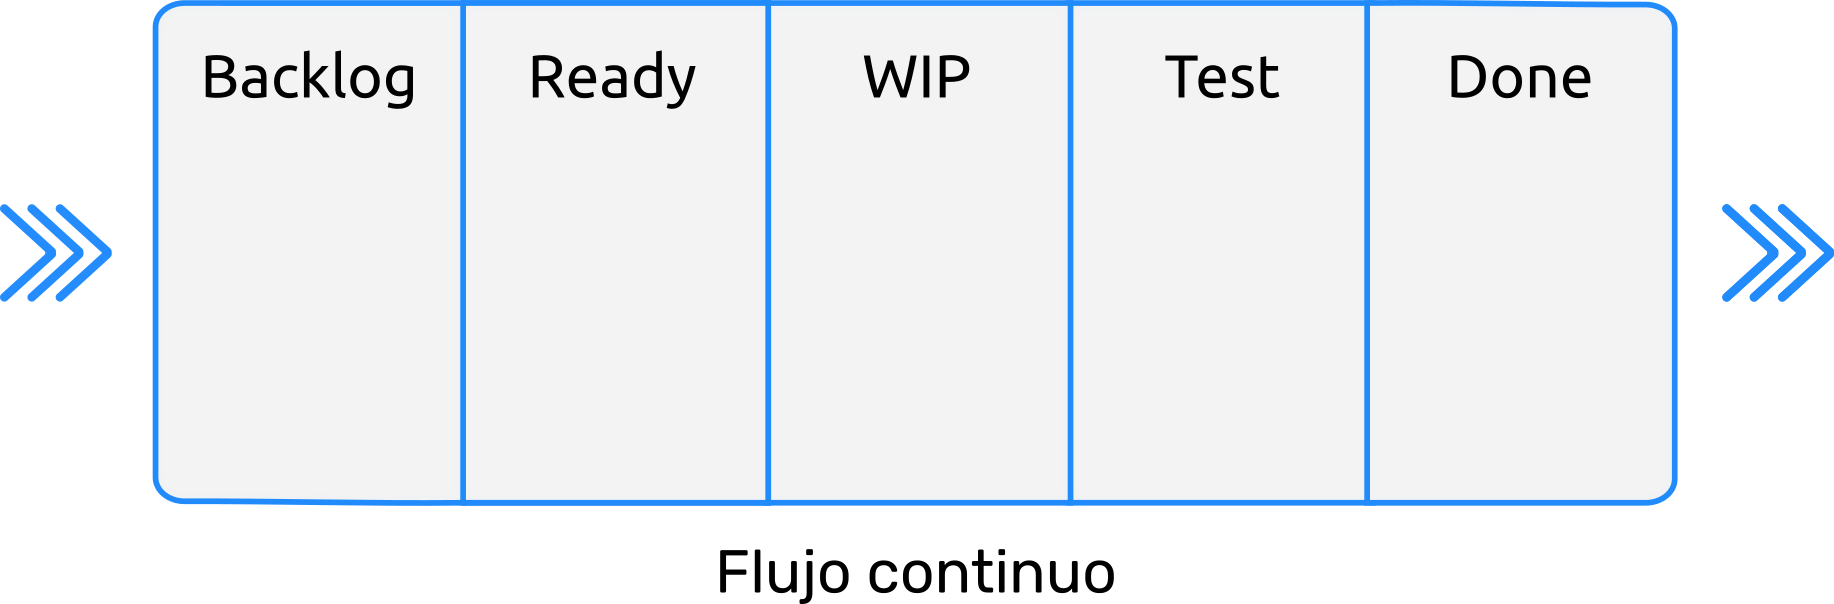
\includegraphics[width=0.8\textwidth]{kanban}
	\caption{Tablero Kanban utilizado.}
\end{figure}

Como herramienta de gestión Kanban, empleamos Kanboard \cite{kanboard}. Se trata de una aplicación \emph{web} \emph{open-source} activamente desarrollada. Contratamos un servidor EC2 con Amazon Web Services (AWS) desde el cual podemos servir la aplicación \emph{web}, la cual a su vez hace uso de una base de datos PostgreSQL en la cual almacena los datos generados. Dicha base de datos está desplegada a través del servicio RDS, también perteneciente a1 AWS.

Se puede acceder al tablero público a través de \href{https://kanban.jizt.it}{\texttt{https://kanban.jizt.it}}.



\section{Motivación tras las arquitecturas desarrolladas}

\subsection{Arquitectura de microservicios}

Desde un primer momento, se concibió la arquitectura con los siguientes objetivos presentes:

\vspace{-0.5cm}
\begin{itemize}
	\item [\textbullet] \textbf{Flexibilidad}: la Inteligencia Artificial y, en concreto, el Procesamiento de Lenguaje Natural, son campos en continuo desarrollo. Cada pocos meses aparecen modelos más potentes que proporcionan mejores resultados. Es por ello que nuestra arquitectura debe proporcionar una estructura lo más desacoplada como sea posible de los modelos concretos de NLP que empleados. De este modo, si aparecieran modelos más avanzados, la transición de unos modelos a otros resultará una labor relativamente sencilla.
	\item [\textbullet] \textbf{Escalabilidad}: los elementos que conforman la arquitectura, deben tener la capacidad de replicarse a fin de responder correctamente a la demanda de usuarios. Adicionalmente, como se ha venido mencionado a lo largo de esta memoria, la implementación de otras tareas de NLP diferentes de la generación de resúmenes es algo que entra dentro de nuestros planes a medio plazo. La arquitectura debe estar estructurada de tal forma que esta expansión se pueda llevar a cabo sin inconvenientes. 
	\item [\textbullet] \textbf{Alta disponibilidad}: relacionada con el punto anterior, se debe poder prestar servicio de forma continua, independientemente de que se produzcan picos en la carga de trabajo, o de que alguno de los componentes falle en un momento dado.
	\item [\textbullet] \textbf{\emph{Cloud native}}: este punto engloba a todos los anteriores; los sistemas \emph{cloud-native} están diseñados para adaptarse a entornos cambiantes, operar a gran escala y poseer resiliencia \cite{cloud20}.
\end{itemize}

Una de las arquitecturas que permiten conseguir los objetivos recogidos anteriormente, es la \textbf{arquitectura de microservicios}. Con este patrón arquitectónico, la aplicación se divide en pequeños servicios, cada uno de los cuales cumple una labor específica, y encapsula todas sus dependencias, a fin de conseguir el máximo grado de independencia posible.

En nuestro caso, además, existen tareas que llevan considerablemente más tiempo que otras, como es el caso de la generación del resumen (que puede durar segundos), frente al pre-procesado del texto (el cual es instantáneo). Una arquitectura como esta nos permite replicar el microservicio encargado de la generación del resumen, para repartir la carga de trabajo entre las diferentes réplicas.

Además, si uno de los microservicios fallara, sería reemplazado inmediatamente por una nueva réplica, gracias a la tecnología de Kubernetes.

\subsection{Arquitectura dirigida por eventos}

Dado que ya ha sido introducida en la \hyperref[subsec:kafka]{sección referente a Kafka}, no entraremos en mucho detalle para evitar repetirnos.

Simplemente recordaremos que este patrón arquitectónico hace posible la comunicación entre los microservicios de forma fiable y rápida. En nuestro caso, un evento sería la finalización del trabajo por parte de uno de los microservicios. Este evento genera una respuesta en otro de los microservicios, el cual lo procesa y comienza su labor específica.

Este patrón nos ofrece también flexibilidad a la hora de introducir nuevos microservicios, ya que, al menos en el caso de Kafka, el \emph{topic} al que un microservicio produce (o consume) eventos podría ser modificado en tiempo de ejecución, sin necesidad de alterar el código fuente del microservicio.

\subsection{API REST Asíncrona}

La generación de resúmenes es un proceso que se puede dilatar varios segundos en el tiempo, dependiendo de factores como la longitud del texto o de los parámetros con los que se genere el resumen. Por lo tanto, realizar peticiones síncronas queda descartado, puesto que una petición HTTP no debe prolongarse durante tanto tiempo.

La forma común de solucionar este problema, logrando asincronismo, pasa por realizar una primera petición dándole a conocer al sistema que queremos generar un resumen. El sistema, entonces, responderá haciéndonos saber que la petición ha sido recibida y se está procesando. A partir de ese momento, consultaremos periódicamente al sistema para conocer el estado del resumen, hasta finalmente obtenerlo, una vez haya sido generado.

Veamos el proceso de manera un poco más detallada.

\subsubsection{1. Petición HTTP POST}

El cliente comienza realizando una petición \texttt{POST} incluyendo en el cuerpo de la misma el texto que quiere resumir. La API le responde con un identificador único del resumen, el \texttt{summary\_id}, así como otros campos de interés:

\begin{figure}[h]
	\centering
	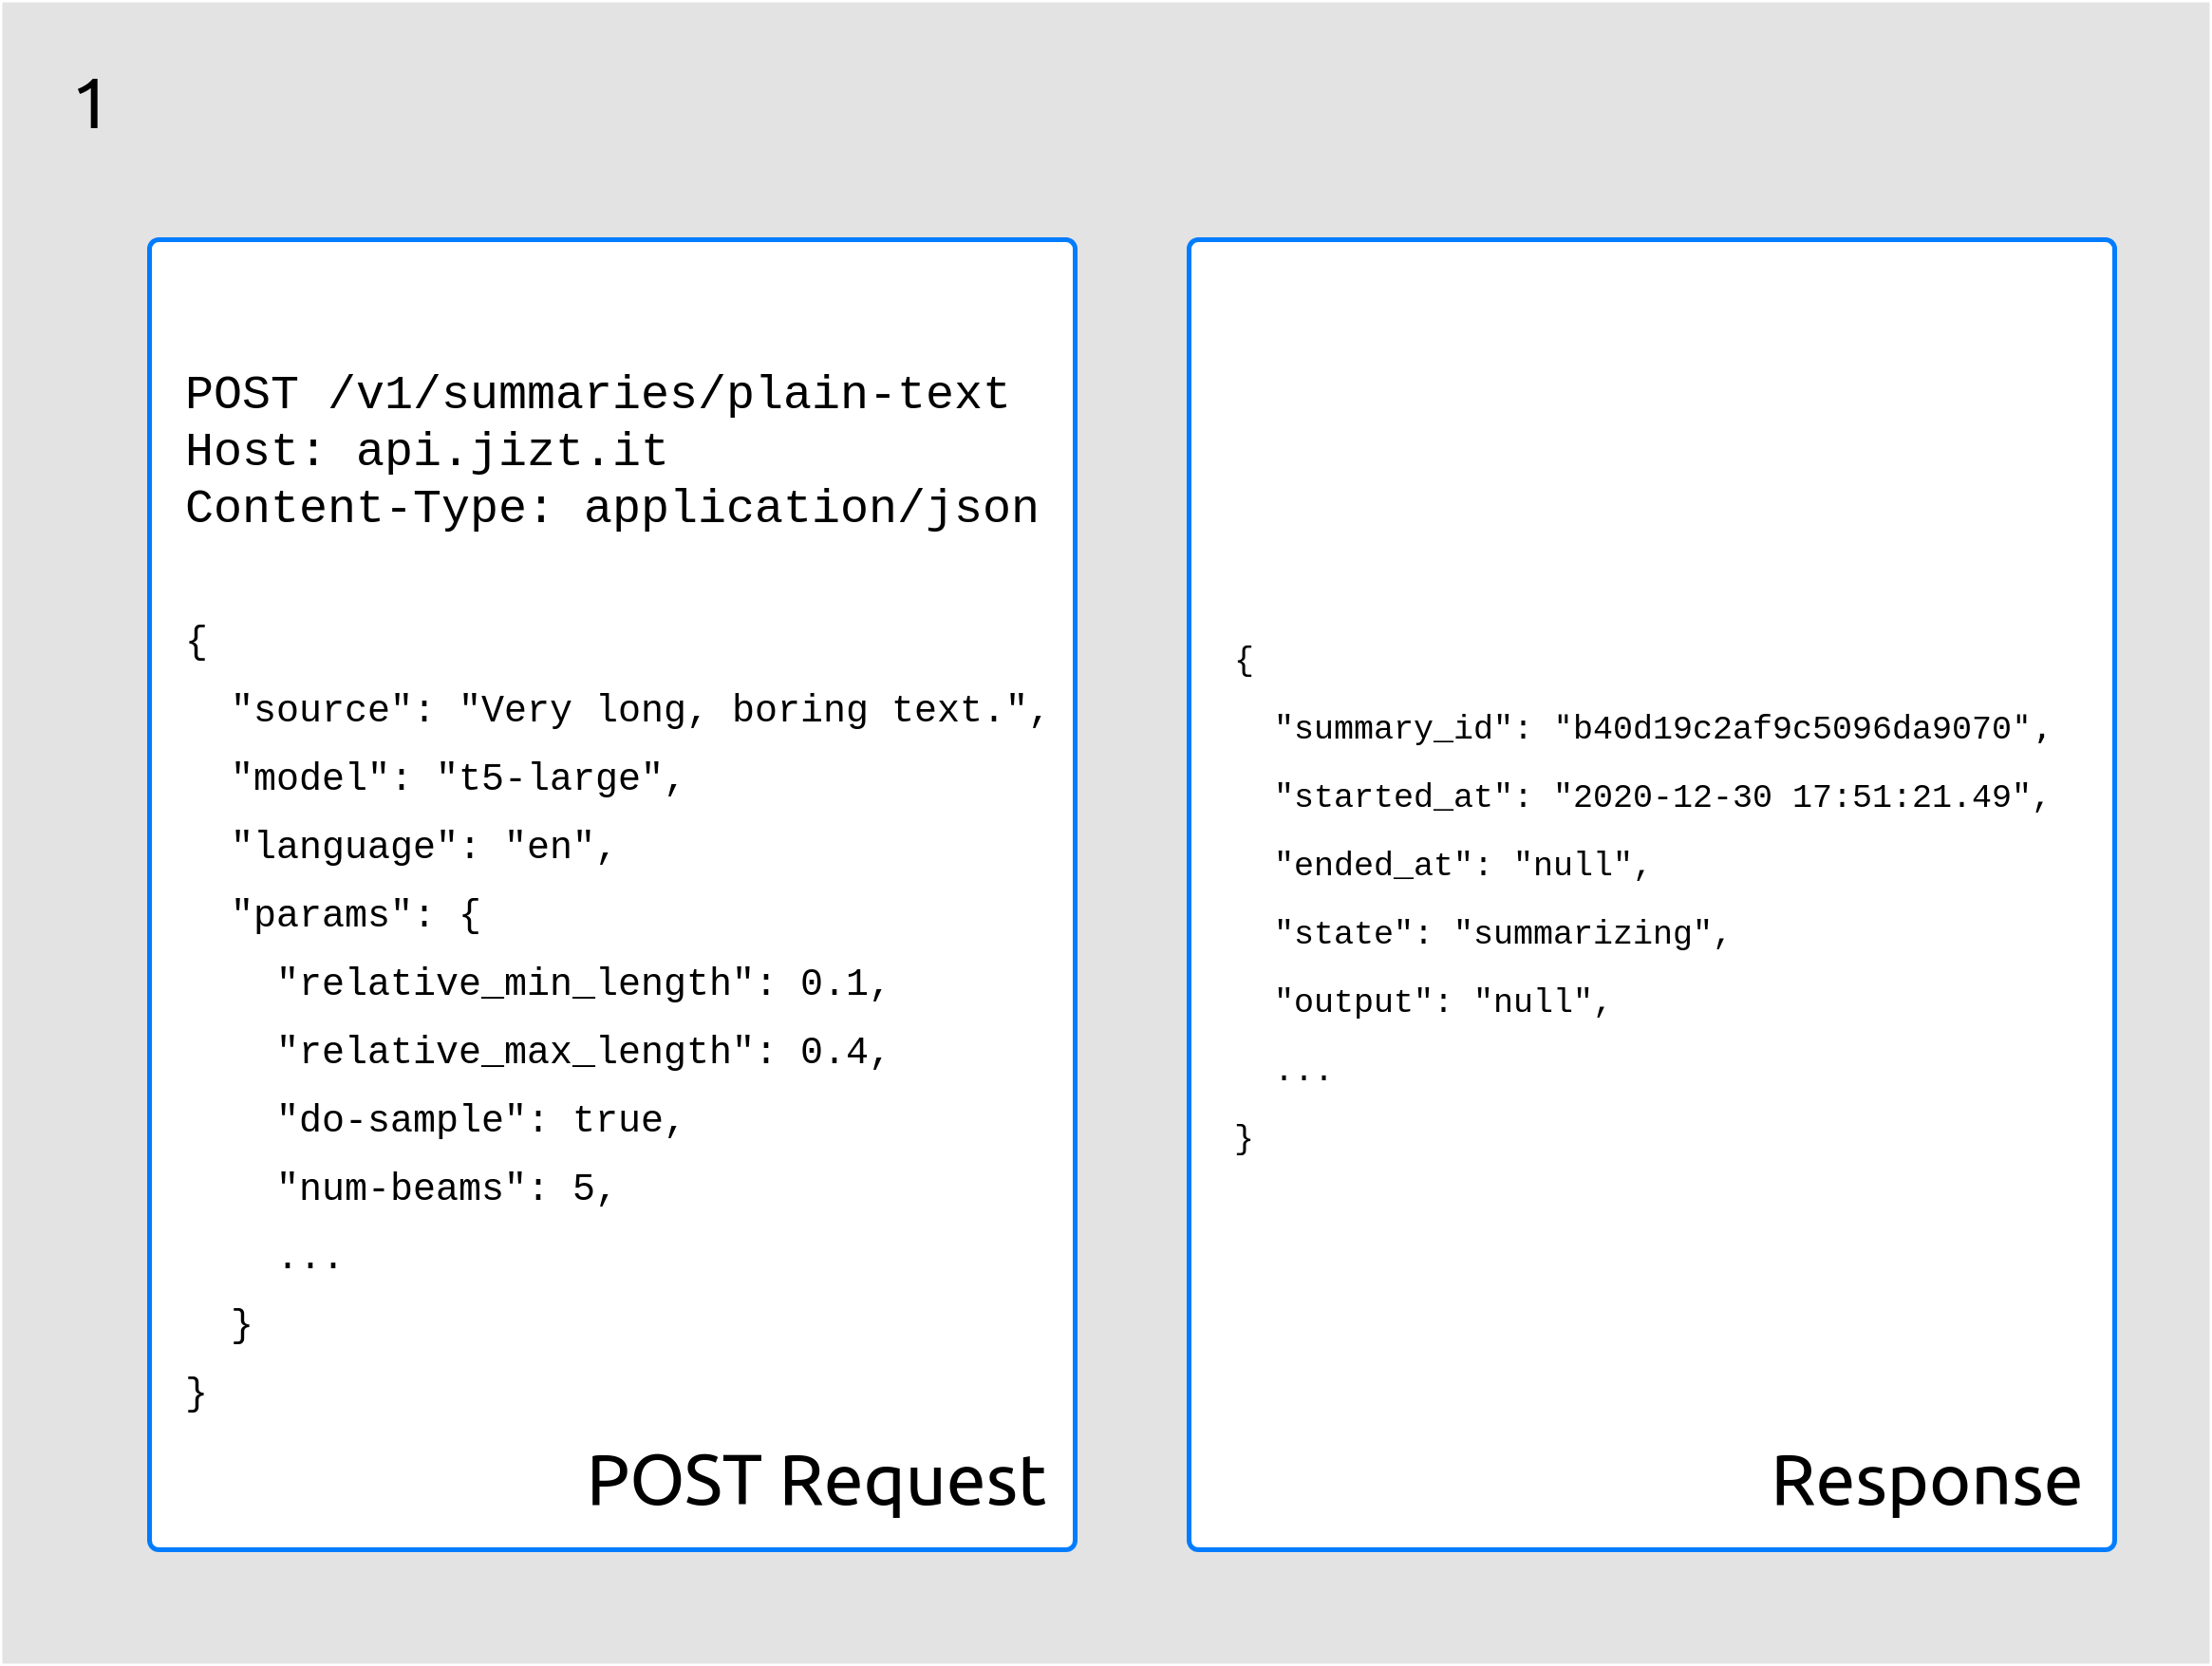
\includegraphics[width=\textwidth]{api-request-1}
	\caption[Primer paso: realizar una petición POST.]{El primer paso es realizar una petición \texttt{POST} con el texto a resumir.}
	\label{fig:api-primer-paso}
\end{figure}

Como vemos en la \hyperref[fig:api-primer-paso]{anterior figura}, el estado del resumen es \texttt{``resumiendo''} (\texttt{``summarizing''}), y aún no tenemos acceso al resumen (\texttt{ouput}), el cual es por el momento \texttt{``null''}.

Una de las principales ventajas de poder consultar el estado del resumen, es poder ofrecer al usuario retroalimentación de los pasos que se están llevando a cabo, mostrándole así que su resumen efectivamente está siendo procesado.

\subsubsection{2. Peticiones HTTP GET sucesivas}

En ese momento, el cliente puede llevar a cabo peticiones HTTP GET con el \emph{id} del resumen de manera periódica a fin de consultar el estado del mismo.

En algún momento, el estado del resumen pasará a ser \texttt{``completado''} (\texttt{``completed''}), y la respuesta a nuestra petición contendrá el resumen generado:

\begin{figure}[h]
	\centering
	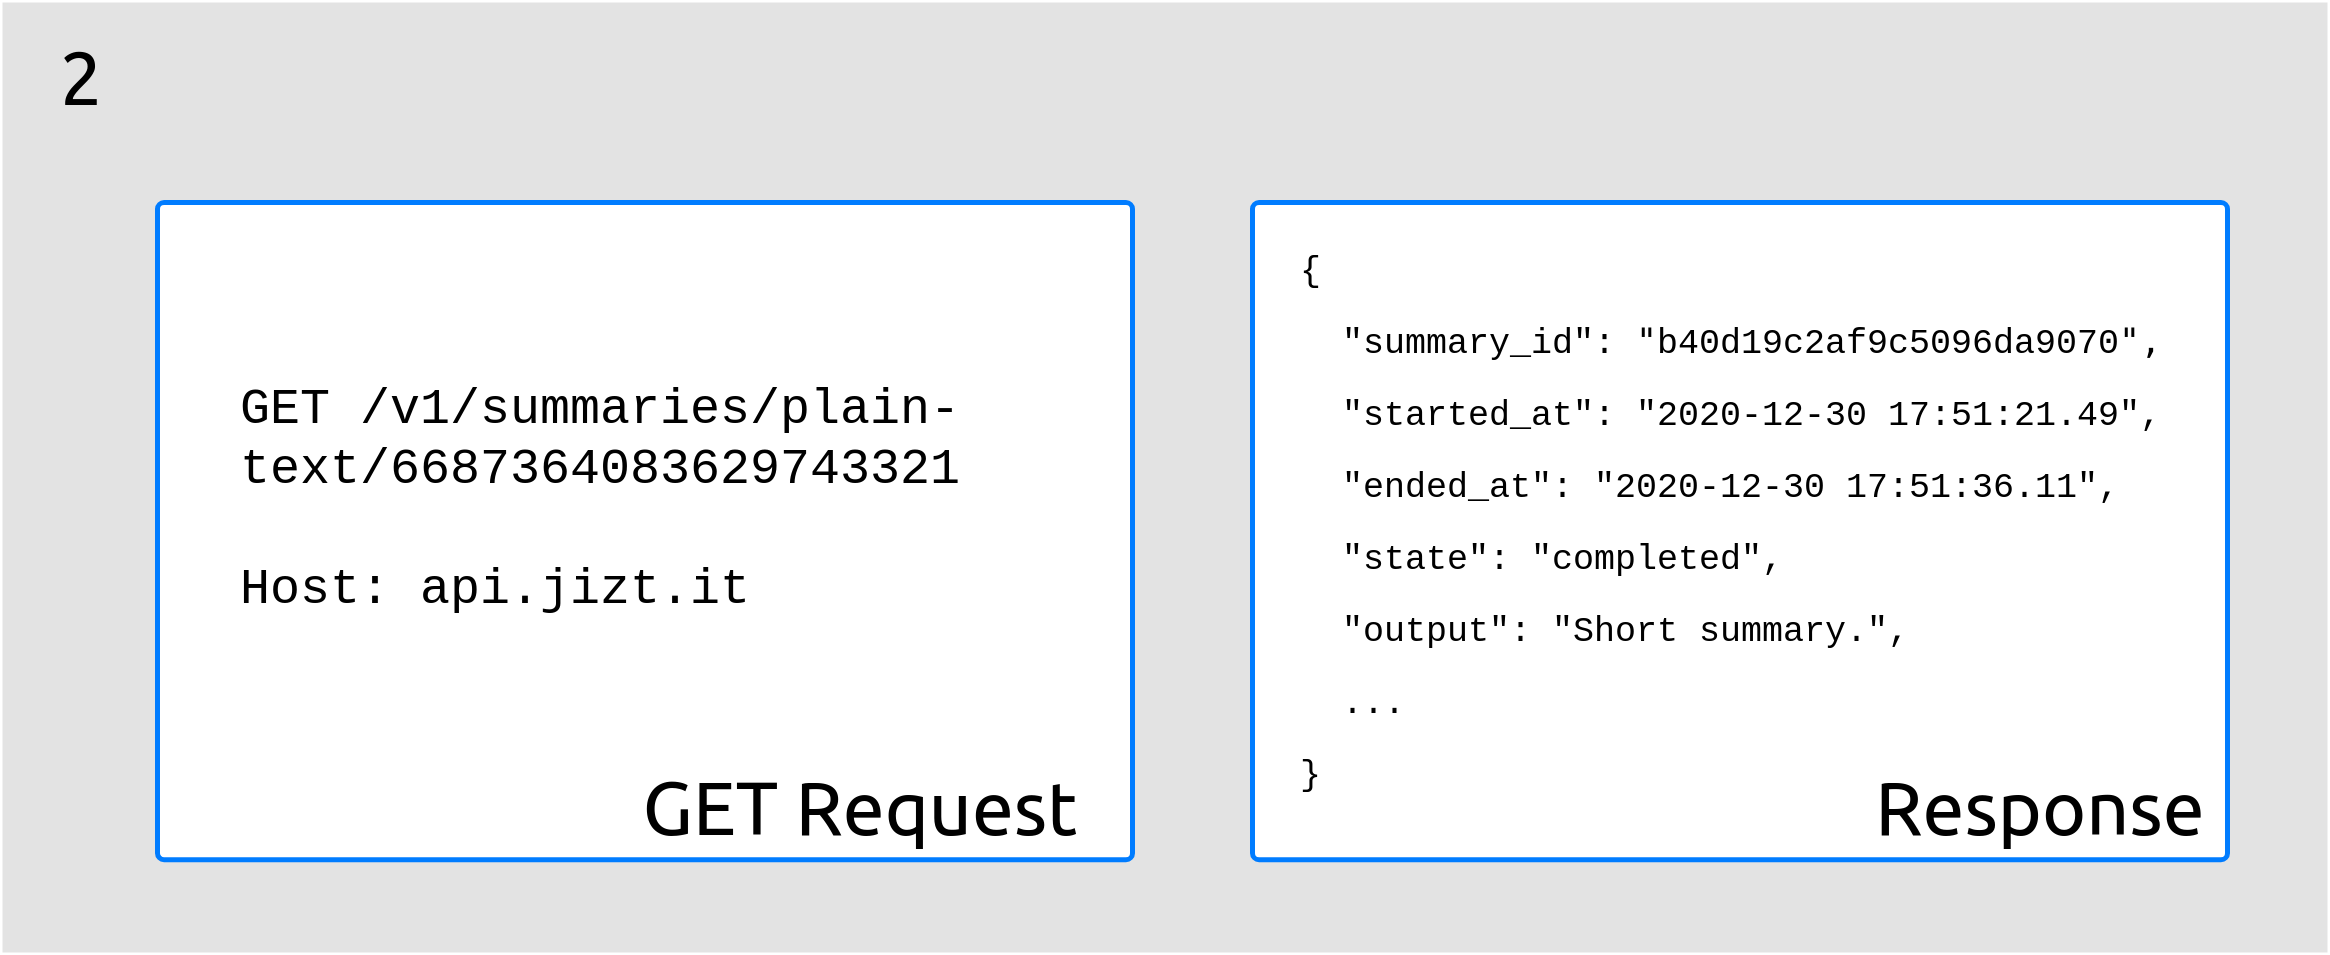
\includegraphics[width=\textwidth]{api-request-2}
	\caption{Finalmente, obtenemos el resumen generado.}
\end{figure}

En el caso de que previamente se hubiera solicitado un resumen del mismo texto, con el mismo modelo y parámetros, el resumen ya estaría almacenado en la base de datos, por lo que la respuesta al primer \texttt{POST} ya contendría dicho resumen.


\subsection{Desarrollo de la aplicación}

A la hora de desarrollar la aplicación, se ha dado gran importancia al diseño de la arquitectura. Con tal fin, nos hemos basado en varios patrones de diseño, dando lugar a una arquitectura que toma elementos de los patrones BLoC \cite{miola20}, \emph{Domain-Driven Design} \cite{vernon13} o \emph{Clean Architecture} \cite{martin15}.

Antes de explicar qué significan estos conceptos, veamos cómo se conforma la arquitectura de la aplicación:

\begin{figure}[!h]
	\centering
	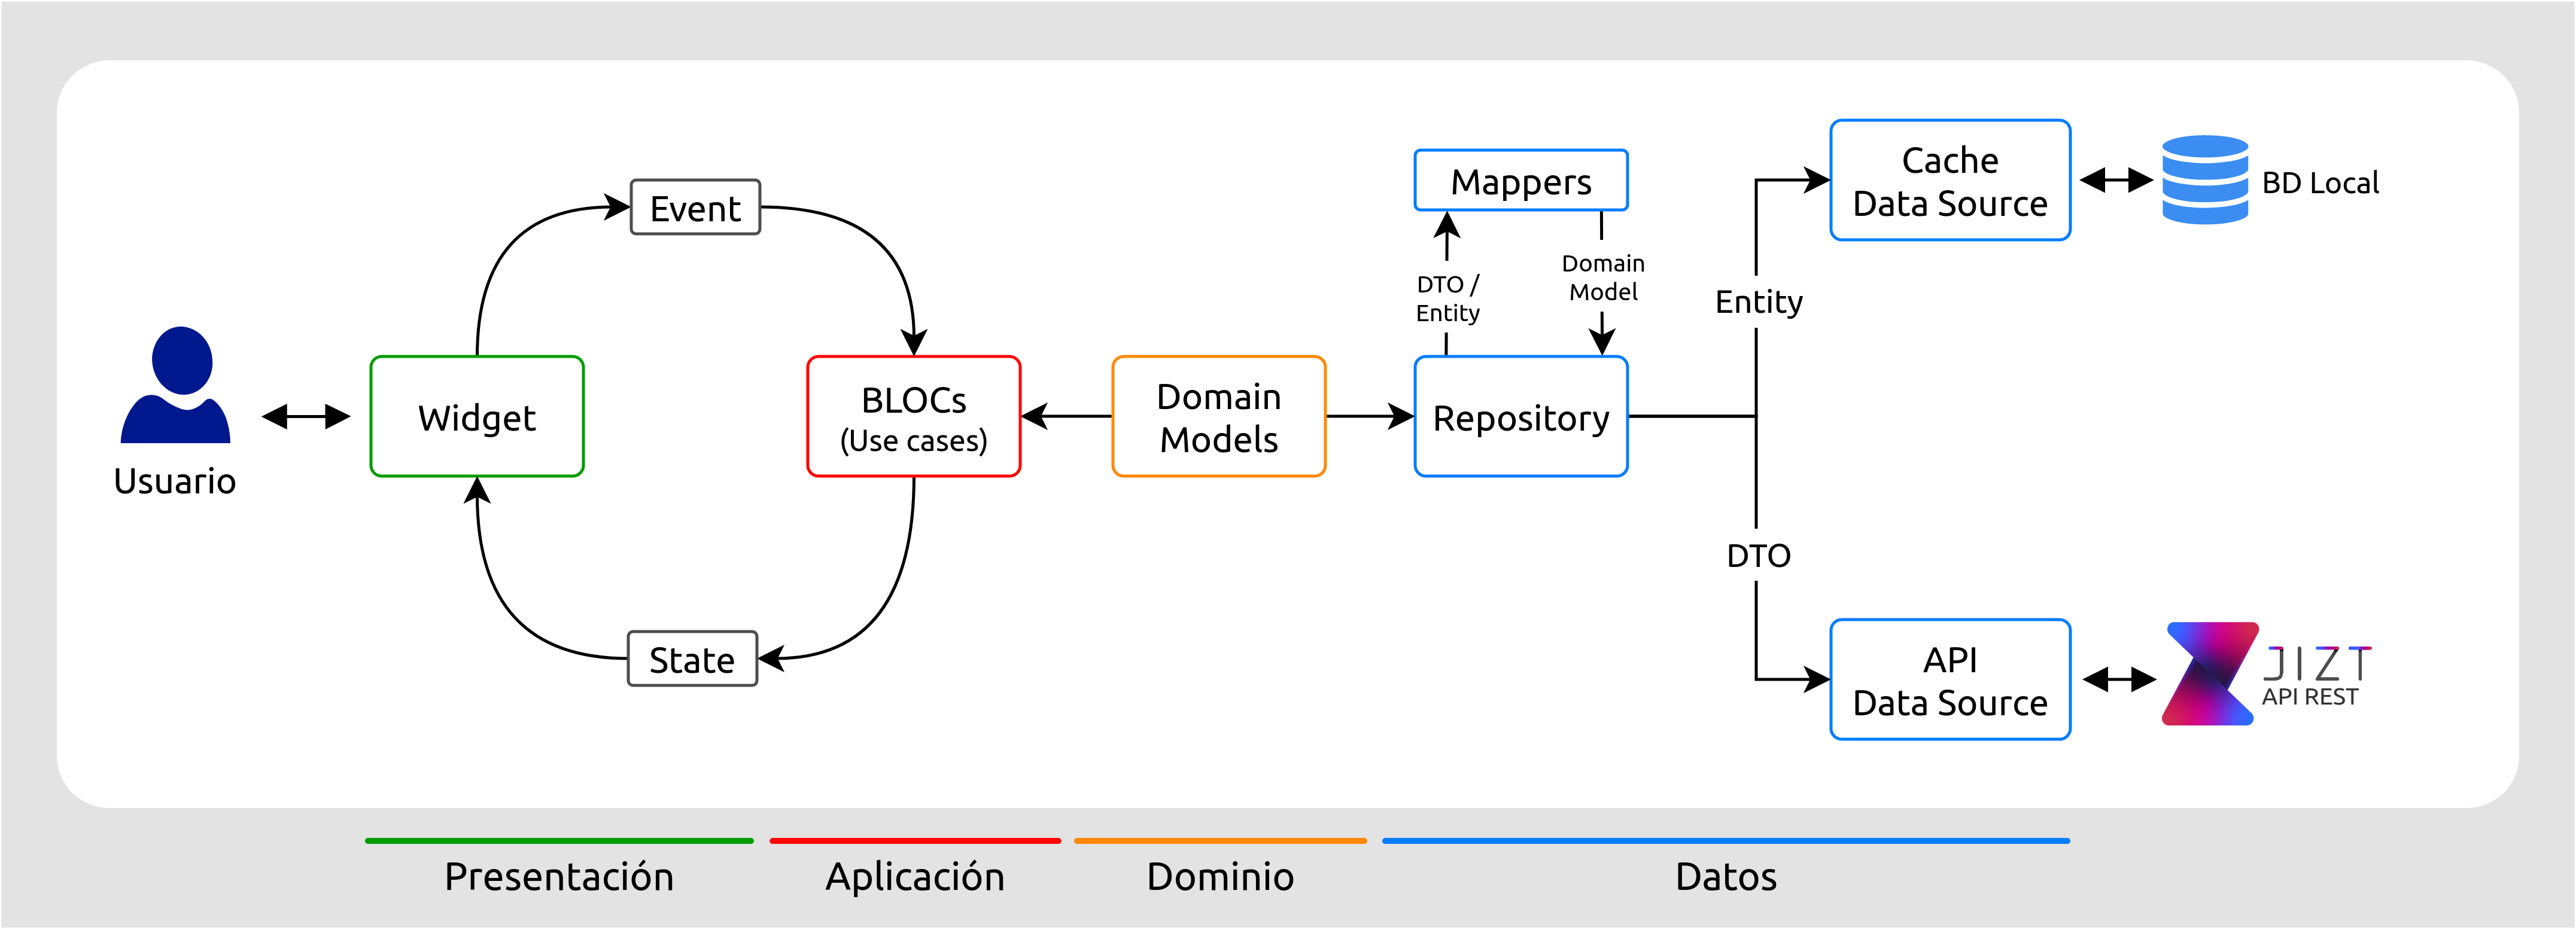
\includegraphics[width=\textwidth]{jizt-app-arch}
	\caption{Arquitectura de la aplicación.}
\end{figure}

Como podemos ver, la arquitectura se divide en cuatro capas: presentación, aplicación, dominio y datos, siendo las primeras las más cercanas al usuario.

Expliquemos de forma más detallada cada una de ellas, comenzando por la capa de \emph{datos}, a la derecha de la imagen.

\subsubsection{Capa de datos}

En esta capa se hace uso del patrón repositorio, el cual sitúa un componente intermedio entre la capa de dominio y el mapeo de los datos a fin de aislar los objetos del dominio de los detalles de implementación concretos a la hora de acceder a la fuente de datos \cite{vernon13}.

Nuestra aplicación implementa un caché local, de forma que, cuando el usuario solicita un resumen, se comprueba primero si dicho resumen ya ha sido generado previamente, acudiendo a la base de datos local, y en caso afirmativo, se recupera directamente el resumen; si no, se aguarda a la respuesta de la API REST.

Esta capa es el punto de conexión entre tres ámbitos  diferentes: la capa de dominio, la cual explicaremos a continuación, la caché local, y la API REST.

La forma en que cada uno de estos ámbitos represente los datos (en nuestro caso, los resúmenes) es independiente del resto. Por ello, vamos a contar con tres representaciones diferentes, cada una correspondiéndose con uno de los ámbitos descritos:

\begin{itemize}[\textbullet]
	\item \emph{Domain Model}: es la representación de los resúmenes propia de la capa de dominio.
	\item DTO (\emph{Data Transfer Object}): se corresponde con la representación del \emph{backend}, esto es, la API REST.
	\item \emph{Entity}: es la representación del caché local.
\end{itemize}

Para que estas tres representaciones diferentes se acoplen correctamente, se hace uso de los \emph{mappers}, los cuales se encargan de transformar la representación de la capa de dominio a DTOs o \emph{Entities}, y viceversa.

\subsubsection{Capa de dominio}

Esta capa define la lógica de negocio de la aplicación, y es independiente de la plataforma de desarrollo, es decir, en nuestro caso estará escrita puramente en Dart, sin contener ningún elemento de Flutter \cite{flutter-clean-arch}. El motivo reside en que el dominio, como decíamos, solo debe ocuparse de la lógica de negocio, y no de los detalles de implementación. Esto también permite una fácil migración entre plataformas, en caso de ser necesario en algún momento.

\subsubsection{Capas de aplicación y presentación}

En estas capas entra en juego el patrón BLoC (\emph{Business Logic Component}). Para entender este patrón, debemos primero explicar los conceptos de \emph{evento} y \emph{estado}.

Dicho de manera sencilla, un estado es aquello que se muestra en la pantalla en un momento específico. Y un evento no es más que una acción detectada por la aplicación, por ejemplo, un \emph{click} del usuario.

Los actores centrales de este patrón son los casos de uso (llamados también BLoCs, como el propio patrón), los cuales contienen las reglas de negocio específicas de la aplicación.

Una vez introducidos los conceptos, podemos identificar cuatro pasos fundamentales:

\vspace{-0.3cm}
\begin{enumerate}
	\item Un componente (\emph{widget}) envía un \emph{evento} al componente BLoC.
	\item El BLoC acepta el evento y lleva a cabo la tarea que tiene asociada, probablemente interaccionando con la capa de dominio.
	\item El BLoC actualiza su \emph{estado}.
	\item Los componentes detectan el cambio de estado y reaccionan de algún modo.
\end{enumerate}

Anteriormente, hemos mencionado el término \emph{widget}. En Flutter, los \emph{widgets} son los elementos que conforman la interfaz de usuario \cite{flutter-widget}, como un botón o un \emph{layout}. Los \emph{widgets} se organizan de forma jerárquica, de modo que toda aplicación tendrá un \emph{widget} raíz, del cual <<colgarán>> el resto de \emph{widgets}, como podemos ver en la \hyperref[flutter-widgets]{siguiente figura}.

\begin{figure}[!h]
	\centering
	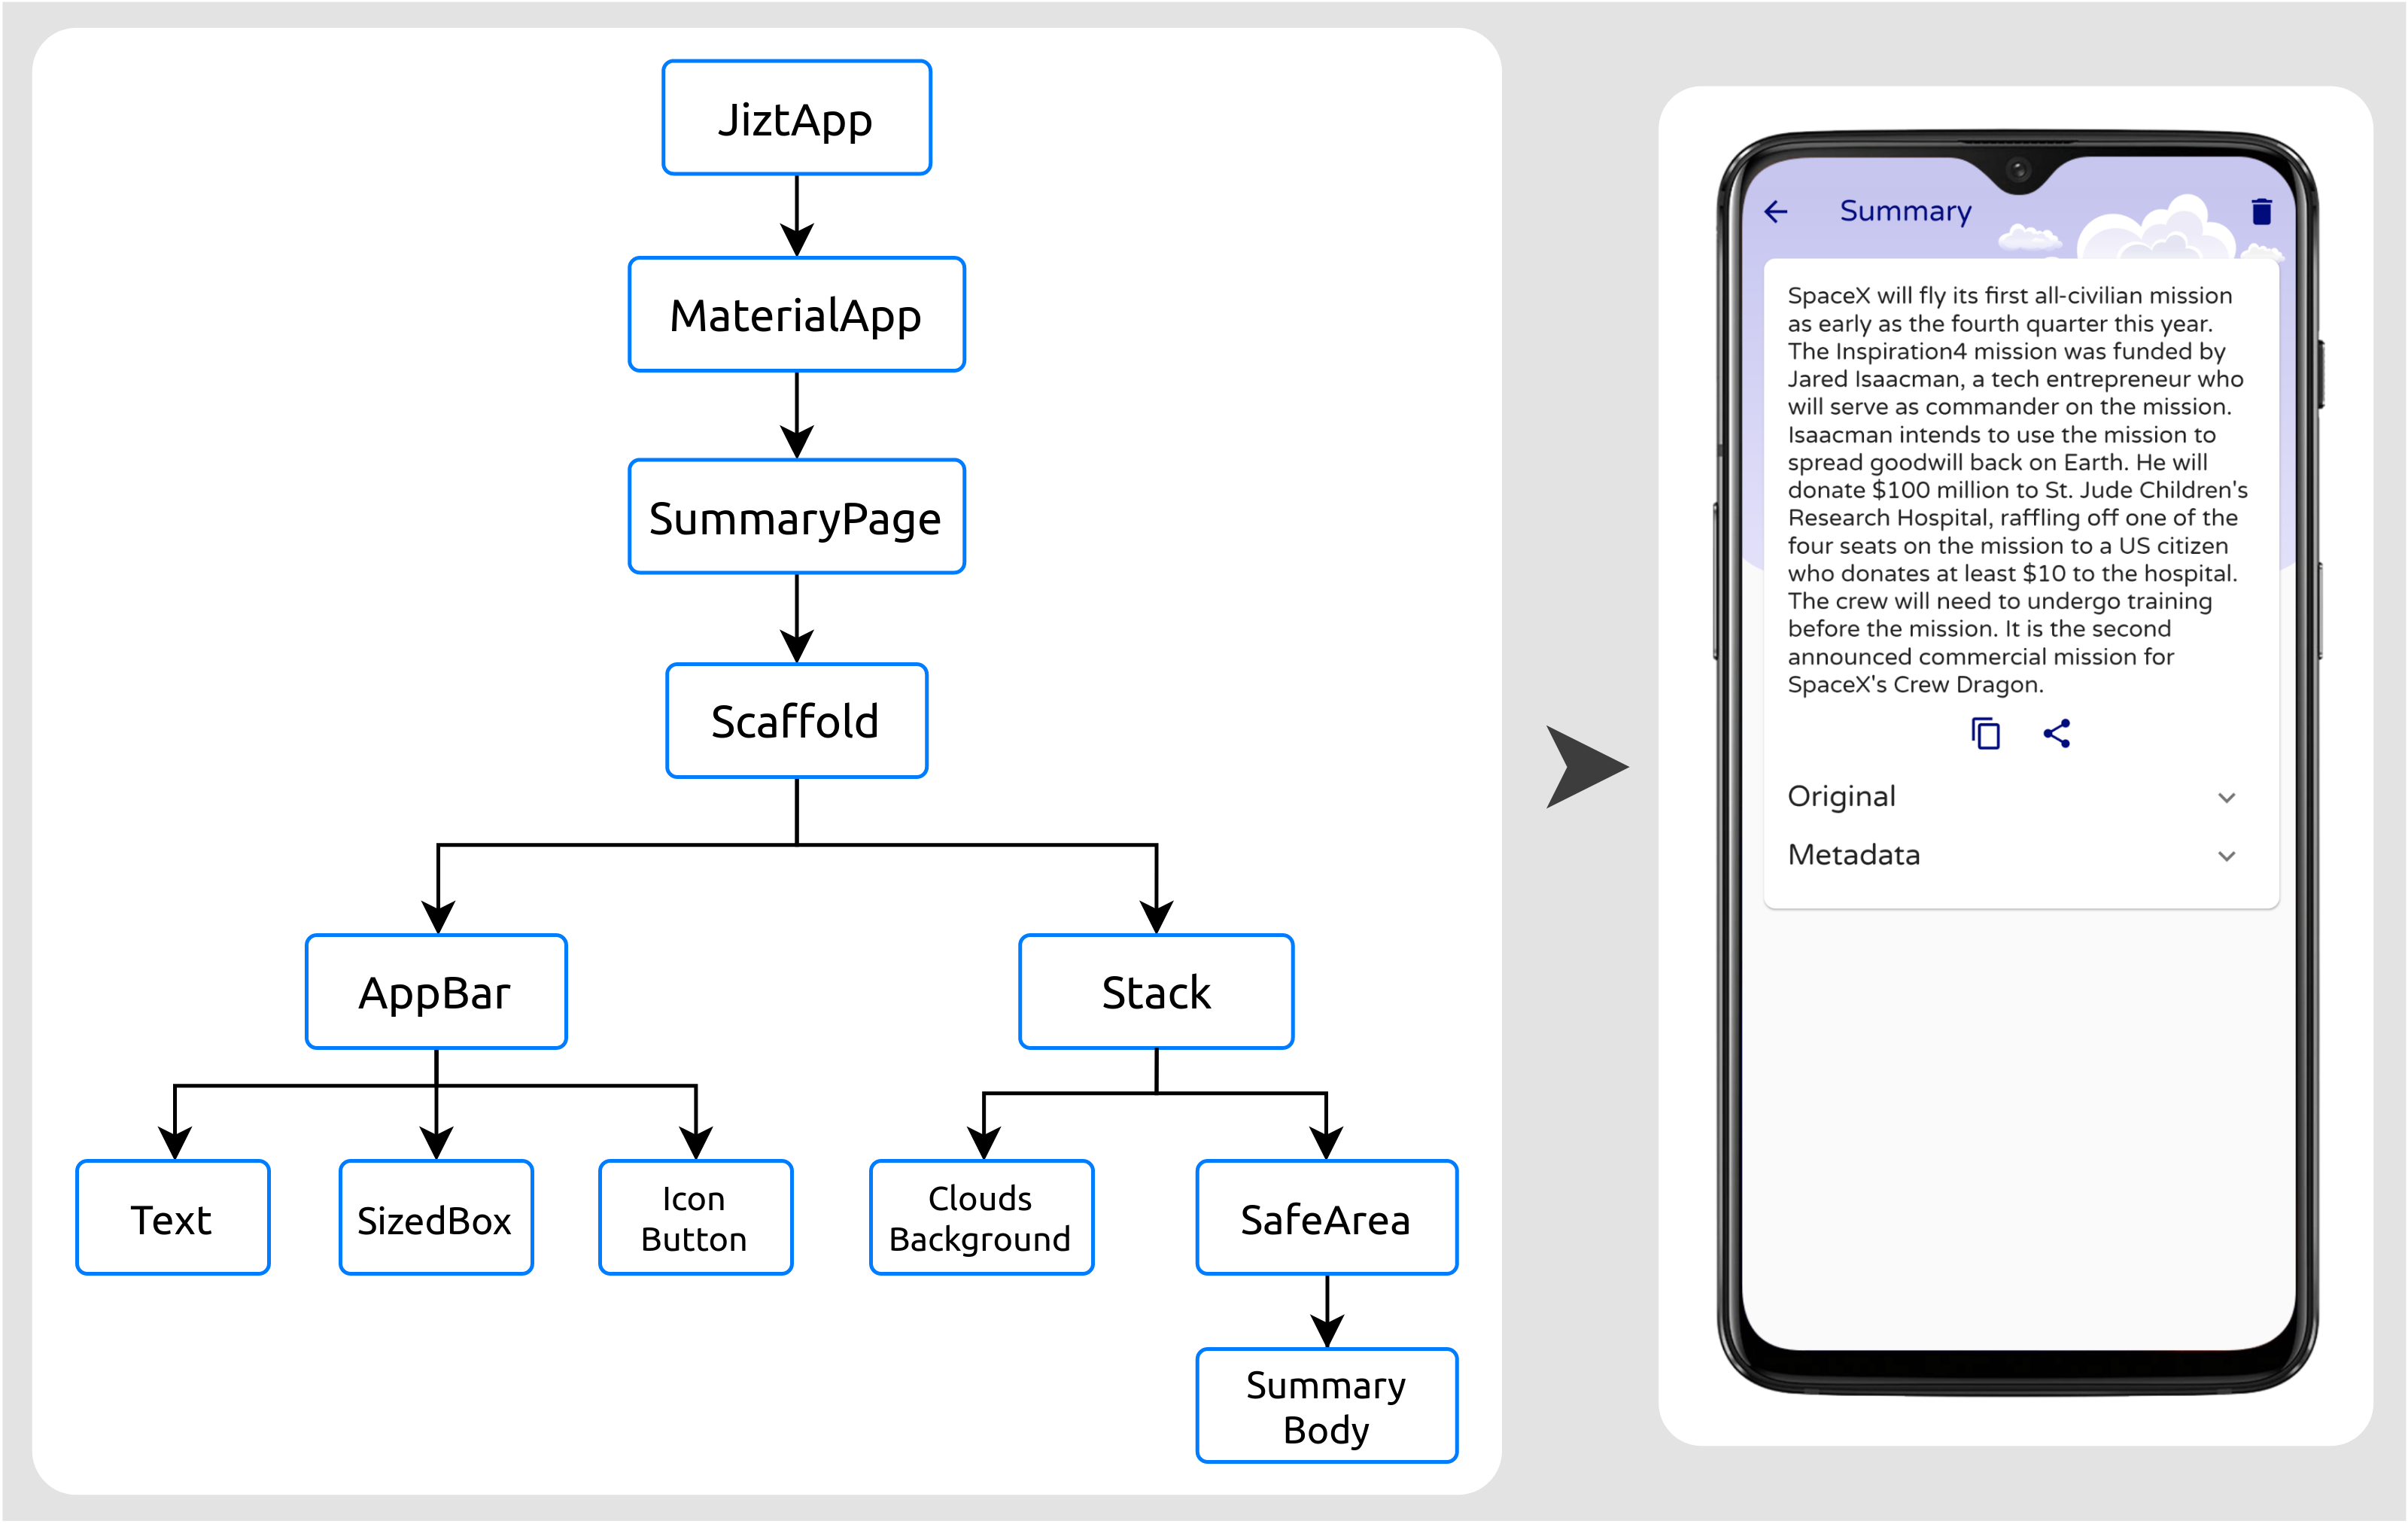
\includegraphics[width=1\textwidth]{widget-hierarchy}
	\caption[Ejemplo de jerarquía de \emph{widgets}.]{Ejemplo de jerarquía de \emph{widgets} de una aplicación sencilla. Imagen del dispositivo móvil extraída de \cite{miola20}.}
	\label{flutter-widgets}
\end{figure}


	\capitulo{6}{Trabajos relacionados}

Este apartado sería parecido a un estado del arte de una tesis o tesina. En un trabajo final grado no parece obligada su presencia, aunque se puede dejar a juicio del tutor el incluir un pequeño resumen comentado de los trabajos y proyectos ya realizados en el campo del proyecto en curso. 

	\capitulo{7}{Conclusiones y Líneas de trabajo futuras}

\vspace{-1cm}
Por último, y no por ello menos importante, se recogen a continuación las principales conclusiones extraídas de la realización de este proyecto. Además, se indican los posibles pasos a tomar en el futuro próximo.

\section{Principales conclusiones}

Como mencionábamos en la \hyperref[chapter:intro]{Introducción}, desde un principio supimos que JIZT era un proyecto ambicioso que requeriría gran inversión de tiempo y esfuerzo.

Cinco meses después, podemos decir, no sin cierto alivio, que hemos sido capaces de cumplir los objetivos que nos marcamos para la compleción de el presente Trabajo de Fin de Grado; JIZT es, ha día de hoy, una realidad.

Personalmente, nunca imaginamos que en torno a un 70 \% del tiempo y esfuerzo se acabaría destinando al \emph{backend}. Esta era, a su vez, el área que menos había trabajado con anterioridad, por lo que fue un reto aún mayor. Cabe preguntarnos, ¿ha valido la pena todo el esfuerzo? Y la respuesta es un rotundo sí. Contar con una buena infraestructura en el \emph{backend} será la clave para el futuro de JIZT por los siguientes motivos:

\vspace{-0.2cm}
\begin{itemize}
	\item [\textbullet] Facilita el escalado y asegura una alta disponibilidad de los componentes implementados actualmente.
	\vspace{-0.2cm}
	\item [\textbullet] Permite la ampliación de las tareas de NLP proporcionadas por JIZT.
	\vspace{-0.2cm}
	\item [\textbullet] Incentiva y facilita la colaboración de otros desarrolladores, dado que se siguen estándares de la industria.
	\vspace{-0.2cm}
	\item [\textbullet] Todo ello se revierte en una mayor satisfacción de los usuarios.
\end{itemize}

\vspace{-0.3cm}
La lección extraída de todo lo mencionado anteriormente es que la Ingeniería del \emph{Software}, así como el Diseño de Arquitectura de \emph{Software} son labores que pueden resultar muy complejas, pero a su vez gratificantes, especialmente en el momento en que finalmente todos los \emph{test} se ejecutan con éxito tras horas de trabajo, e interminables <<quebraderos de cabeza>>, si se nos permite la expresión.

No obstante, hablando de dificultades, el Procesamiento de Lenguaje Natural es también un muy buen candidato; con la realización de este proyecto nos hemos percatado de la enorme flexibilidad y ambigüedad del lenguaje natural, lo cual imposibilita establecer reglas prefijadas que sean válidas para todos los casos, como se intentó desde el inicio del NLP hasta ya entrado el siglo XXI. Cuando crees que has dado con una regla que se ajusta a todos los supuestos considerados, aparece un nuevo caso que lo desmonta todo. Por suerte, en los últimos cinco años se han producido grandes avances en el campo; no podemos esperar a poder analizar y probar los nuevos descubrimientos que el futuro nos traiga.

Podríamos mencionar muchas otras conclusiones, pero todas ellas se pueden resumir del siguiente modo: hemos aprendido \emph{mucho}. Nuestro proyecto ha tratado con diseño de microservicios e infraestructura en la nube (Kubernetes, Docker, Kafka, API REST), bases de datos (PostgreSQL como servicio), Inteligencia Artificial (Procesamiento del Lenguaje Natural), desarrollo de aplicaciones multiplataforma (Flutter), validación y pruebas, despliegue e integración continua...

Este proyecto ha sido una oportunidad de aprendizaje y formación que creemos será muy positiva de cara a nuestra futura vida estudiantil y laboral.


\section{Líneas futuras de trabajo}

JIZT, dada su extensión, cuenta con innumerables aspectos a desarrollar en numerosos aspectos. A continuación listamos algunos de los más importantes y/o inmediatos:

\vspace{-0.3cm}
\begin{itemize}[\textbullet]
	\item Incluir modelos en otros idiomas idiomas, como español, francés, alemán, chino, etc.
	\item Ampliar el rango de tareas de NLP que JIZT es capaz de llevar a cabo.
	\item Entrenar/reemplazar el modelo de \emph{truecasing} (recomposición de mayúsculas), ya que el usado actualmente está entrenado con un corpus pequeño, el cual generalmente consigue buenos resultados, pero en algunos casos es mejorable.
	\item Seguir mejorando la API REST y el \emph{backend}. En este aspecto, las mejoras más destacables son:
	\begin{itemize}[◦]
		\item Incluir la capacidad de extraer textos de ficheros, imágenes o URLs.
		
		\item Incluir un <<modo privado>>, dando al usuario la opción de que su texto no sea almacenado en la base de datos.
		
		\item Actualmente, para detectar si un resumen ya ha sido generado previamente, se extrae un \emph{hash} (SHA-256) a partir del texto original, el modelo, y los parámetros del resumen solicitados. Una mejora pasa por atender al texto pre-procesado, en vez del original, dado que ahora mismo si cambia un solo carácter del texto original, por ejemplo, un espacio, el texto se considera como diferente, y se genera un nuevo resumen. Esta mejora conlleva cierta dificultad dado que alteraría en cierto modo el orden secuencial del proceso de resumen, esto es: el \emph{Dispatcher} enviaría el texto original al pre-procesador, el cual, una vez pre-procesado el texto, se lo devolvería al \emph{Dispatcher}. En el caso de que el texto pre-procesado no existiera, el \emph{Dispatcher} reenviaría el texto directamente al Codificador, dado que ya estaría pre-procesado.
		
		\item Incluir la monitorización y la recogida de métricas del sistema. Actualmente, se implementa un \emph{logging} básico, suficiente para la detección de errores, pero poco apropiado para llevar a cabo estudios de uso de recursos, carga de trabajo, etc.
		
		\item Ofrecer al usuario mensajes de error más granulares. Por ejemplo, si el usuario ha definido parámetros de resumen inexistentes, la API le indicaría exactamente qué parámetros han sido, y por qué valores por defecto se han reemplazado.
	\end{itemize}
	\item En cuanto a la aplicación desarrollada:
	\begin{itemize}[◦]
		\item Iterar junto a la API REST para incluir las mejoras de esta en cuestiones como el <<modo privado>>, la generación de resúmenes a partir de ficheros, imágenes o URLs, mensajes de error más descriptivos, etc.
		
		\item Mejorar la internacionalización de la aplicación, traduciéndola a otros idiomas.
	\end{itemize}
\end{itemize}
	
	
	\printbibliography[title={Bibliografía}]
	
\end{document}
